% ---------------------------------------------------------------
% Preámbulo — Trabajo final Lush Beauty (réplica del formato v4)
% Compilar con XeLaTeX (ver Makefile)
% ---------------------------------------------------------------
\documentclass[12pt,letterpaper]{article}

\usepackage{fontspec}
\setmainfont{TeX Gyre Termes}
\usepackage[english,spanish,es-tabla,es-noshorthands]{babel}
\usepackage[top=2.54cm,bottom=2.54cm,left=2.54cm,right=2.54cm]{geometry}
\usepackage{setspace}
\usepackage{microtype}
\usepackage{graphicx}
\usepackage{float}
\usepackage{xcolor}
\usepackage{array}
\usepackage{booktabs}
\usepackage{longtable}
\usepackage{colortbl}
\usepackage{tabularx}
\usepackage{pdflscape}
\usepackage{enumitem}
\usepackage{fancyhdr}
\usepackage{titlesec}
\usepackage{caption}
\usepackage[titles]{tocloft}
\usepackage{xurl}
\usepackage{amsmath}
\usepackage{amssymb}
\usepackage[hidelinks,bookmarksnumbered]{hyperref}

% Interlineado del cuerpo (el original usa doble espacio); ajustar aquí.
\newcommand{\LBstretch}{1.9}
\setstretch{\LBstretch}
\setlength{\parindent}{0.5in}
\setlength{\parskip}{0pt}
\setlength{\emergencystretch}{2em}
\raggedbottom

% ---------------- Cabecera / pie: número de página arriba a la derecha (APA)
\setlength{\headheight}{14.5pt}
\pagestyle{fancy}
\fancyhf{}
\fancyhead[R]{\thepage}
\renewcommand{\headrulewidth}{0pt}
\fancypagestyle{plain}{\fancyhf{}\fancyhead[R]{\thepage}\renewcommand{\headrulewidth}{0pt}}
\fancypagestyle{portada}{\fancyhf{}\renewcommand{\headrulewidth}{0pt}}

% ---------------- Títulos
\titleformat{\section}{\normalfont\normalsize\bfseries}{\thesection.}{0.4em}{}
\titleformat{\subsection}{\normalfont\normalsize\bfseries}{\thesubsection}{0.4em}{}
\titleformat{\subsubsection}{\normalfont\normalsize\bfseries\itshape}{\thesubsubsection}{0.4em}{}
\titlespacing*{\section}{0pt}{0pt}{0pt}
\titlespacing*{\subsection}{0pt}{0pt}{0pt}
\titlespacing*{\subsubsection}{0pt}{0pt}{0pt}
\let\oldsection\section
\renewcommand{\section}{\clearpage\oldsection}   % cada capítulo en página nueva
\setcounter{secnumdepth}{3}
\setcounter{tocdepth}{3}

% Título centrado sin numerar (Resumen, Índices...)
\newcommand{\titulocentrado}[1]{\clearpage\begin{center}\textbf{#1}\end{center}}

% ---------------- Párrafos especiales del original
\newcommand{\blank}[1]{\rule[-2pt]{#1\dimexpr0.42em\relax}{0.4pt}}
\newenvironment{vinetas}{\begin{itemize}[leftmargin=0.5in,label={\textbullet},itemsep=0pt,topsep=0pt,parsep=0pt]}{\end{itemize}}
\newcommand{\referencia}[1]{\par\noindent\hangindent=0.5in\hangafter=1 #1\par}
\newcommand{\pregunta}[1]{\par\begingroup\setstretch{1.5}\leftskip=0.24in\noindent\strut #1\par\endgroup\vspace{2pt}}
\newcommand{\opciones}[1]{\par\begingroup\setstretch{1.5}\leftskip=0.47in\noindent #1\par\endgroup\vspace{4pt}}
\newcommand{\defterm}[2]{\noindent\hangindent=0pt\textit{#1.} #2\par}

% ---------------- Captions estilo APA 7: "Tabla N" en negrita, título en cursiva debajo
\captionsetup{labelsep=newline,justification=raggedright,singlelinecheck=false,
  labelfont=bf,textfont=it,font=normalsize,skip=4pt,belowskip=0pt}
\captionsetup[longtable]{position=top}
\newcommand{\nota}[1]{\par\vspace{2pt}{\setstretch{1.0}\small\noindent\textit{Nota.} #1\par}\vspace{10pt}}
\newcommand{\tablefont}{\small\setstretch{1.0}}

% Numeración de tablas de anexo: A1, C1, G1...
\newcommand{\anexotabla}[1]{\setcounter{table}{0}\renewcommand{\thetable}{#1\arabic{table}}\renewcommand{\theHtable}{#1\arabic{table}}}
\newcommand{\finanexotabla}{\renewcommand{\thetable}{\arabic{table}}}

% Anexos (sin numeración, con entrada en el índice)
\newcommand{\anexo}[1]{\clearpage\phantomsection\noindent\textbf{#1}\par\addcontentsline{toc}{section}{#1}\nopagebreak}
\newcommand{\subanexo}[1]{\phantomsection\noindent\textbf{#1}\par\addcontentsline{toc}{subsection}{#1}\nopagebreak}

% ---------------- Índices (tocloft)
\renewcommand{\cftsecfont}{\normalfont}
\renewcommand{\cftsecpagefont}{\normalfont}
\renewcommand{\cftsecleader}{\cftdotfill{\cftdotsep}}
\setlength{\cftbeforesecskip}{4pt}
\setlength{\cftbeforesubsecskip}{0pt}
\setlength{\cftbeforesubsubsecskip}{0pt}
\setlength{\cftsubsecindent}{0.3in}
\setlength{\cftsubsubsecindent}{0.6in}
\renewcommand{\cfttabpresnum}{}
\renewcommand{\cfttabaftersnum}{\hspace{0.5em}}
\setlength{\cfttabnumwidth}{3.2em}
\renewcommand{\cftfigpresnum}{}
\setlength{\cftfignumwidth}{3.2em}
\setlength{\cftbeforetabskip}{3pt}
\setlength{\cftbeforefigskip}{3pt}
\renewcommand{\cfttabfont}{\normalfont}
\renewcommand{\cftfigfont}{\normalfont}
\renewcommand{\cftaftertoctitleskip}{0pt}
\renewcommand{\cftafterloftitleskip}{0pt}
\renewcommand{\cftafterlottitleskip}{0pt}

\hypersetup{pdftitle={Sistema Web Móvil para la Gestión de Caja y Nómina del Salón de Belleza Lush Beauty},pdfauthor={Alan Fabian Melgar Alvis; Jhenny Michelle Solis Herrera},pdflang={es}}
\addto\captionsspanish{\renewcommand{\contentsname}{Índice general}\renewcommand{\listtablename}{Índice de tablas}\renewcommand{\listfigurename}{Índice de figuras}}
\renewcommand{\cfttoctitlefont}{\hfill\bfseries}\renewcommand{\cftaftertoctitle}{\hfill}
\renewcommand{\cftlottitlefont}{\hfill\bfseries}\renewcommand{\cftafterlottitle}{\hfill}
\renewcommand{\cftloftitlefont}{\hfill\bfseries}\renewcommand{\cftafterloftitle}{\hfill}
\begin{document}
\thispagestyle{portada}
\begin{center}
\setstretch{1.0}
\vspace*{0.2cm}
\textbf{UNIVERSIDAD AUTÓNOMA GABRIEL RENÉ MORENO}\\[1.1em]
\textbf{Facultad de Ingeniería en Ciencias de la Computación y Telecomunicaciones}\\[1.1em]
\textbf{– GRUPO 8 –}\\[1.4em]

\includegraphics[height=6.8cm]{img/logo_uagrm.png}\\[1.4em]
\textbf{Sistema Web Móvil para la Gestión de Caja y Nómina del Salón de Belleza Lush Beauty}
\end{center}

\vspace{1.2em}
\begingroup
\setstretch{1.0}
\noindent Integrantes:
\begin{itemize}[leftmargin=3.2cm,label={\textbullet},itemsep=2pt,topsep=4pt,parsep=0pt]
\item Melgar Alvis Alan Fabian 221089659
\item Solis Herrera Jhenny Michelle 218165994
\end{itemize}
\vspace{0.8em}
\noindent\textbf{Materia:} Economía para la gestión\\[0.8em]
\noindent\textbf{Docente:} Ing. Ricardo Terrazas Soto\\[0.8em]
\noindent\textbf{Gestión:} Semestre 2 – 2026\\[0.8em]
\noindent\textbf{Lugar:} Santa Cruz – Bolivia
\endgroup

\clearpage
\pagenumbering{roman}
\titulocentrado{Resumen}

La gestión administrativa de los salones de belleza de pequeña escala suele apoyarse en hojas de cálculo elaboradas manualmente, lo que favorece errores de cálculo, inconsistencias de datos y una liquidación de sueldos lenta. El presente trabajo plantea el diseño y la validación de un sistema web móvil, denominado \textit{Lush Beauty}, orientado a la gestión de caja y a la liquidación semanal de comisiones del salón homónimo, cuyo diagnóstico se basa en una planilla de pagos de ejemplo, representativa de la información que recibe el salón (agosto de 2026) (91 servicios, tres especialistas). La investigación es de enfoque cuantitativo con apoyo cualitativo, alcance descriptivo-explicativo y diseño preexperimental de preprueba y posprueba. Se incluyen el planteamiento del problema, los objetivos, la justificación, el marco teórico, un benchmarking de sistemas comerciales similares, las hipótesis con su operacionalización, el marco metodológico y el cronograma de actividades. Se espera que el sistema reduzca el tiempo de liquidación semanal y la tasa de errores de cálculo, además de alcanzar una usabilidad percibida aceptable por parte de las usuarias. Como ampliación orientada a la toma de decisiones, se propone evolucionar el sistema hacia un Sistema de Soporte para la Toma de Decisiones, denominado Lush Beauty Smart DSS, que conserva el núcleo transaccional de caja y nómina y agrega análisis de contribución por servicio, simulación de escenarios What-If, comparación multicriterio con análisis de sensibilidad, recomendaciones explicables y seguimiento de decisiones, además de registro sin conexión, importación asistida de Excel, un asistente financiero (Lush Insight), alertas (Lush Guard) y automatizaciones con n8n. La decisión final siempre corresponde a la administradora: la inteligencia artificial no autoriza pagos ni cambia por sí sola las políticas económicas, y los datos ilustrativos o los escenarios hipotéticos no se presentan como resultados medidos.

\noindent\textbf{Palabras clave:} sistema de información, gestión de salones de belleza, liquidación de comisiones, aplicación web progresiva, benchmarking, sistemas de soporte para decisiones, simulación What-If, análisis multicriterio, inteligencia artificial explicable.

\titulocentrado{Abstract}

\selectlanguage{english}
Lush Beauty Smart DSS extends a mobile-first cash and payroll management system for a small beauty salon into a decision support platform. It integrates service-level contribution analysis, What-If simulation, transparent weighted decision comparison with sensitivity testing, an explainable recommendation engine, and a decision outcome log. The proposal retains offline-first operations, reviewed spreadsheet imports, finance-focused AI assistance, rule-based anomaly alerts and n8n automations. Business decisions remain under human control. The illustrative dataset in the source report is not treated as observed business impact. This document defines architecture, assumptions, a worked example, testable requirements, evaluation metrics and a phased academic implementation plan.

\noindent\textbf{Keywords:} decision support systems; multi-criteria analysis; What-If simulation; contribution analysis; explainable artificial intelligence; cash management; commissions; progressive web app; n8n.
\selectlanguage{spanish}

\clearpage
{\setstretch{1.15}\tableofcontents}
\clearpage
{\setstretch{1.15}\listoftables}
\clearpage
{\setstretch{1.15}\listoffigures}
\clearpage
\pagenumbering{arabic}
\section{Introducción}\label{cap:introduccion}

Los emprendimientos de servicios de belleza constituyen una actividad económica dinámica en las ciudades latinoamericanas y, en su mayoría, operan como microempresas con estructuras administrativas reducidas. En ellas, el registro de servicios, el control de la caja y el cálculo de las comisiones del personal se realizan habitualmente en hojas de cálculo elaboradas por la propia administradora. Si bien esta herramienta es accesible y flexible, la literatura especializada advierte que las hojas de cálculo de uso operativo presentan una incidencia recurrente de errores que rara vez se detectan a tiempo (Panko, 1998).


El presente trabajo aborda el análisis y la propuesta de solución a la gestión administrativa del salón de belleza \textit{Lush Beauty}, un emprendimiento en funcionamiento que lleva su control financiero en hojas de cálculo con una hoja por especialista. El diagnóstico preliminar, realizado sobre una planilla de ejemplo (agosto de 2026) que reproduce el formato y el tipo de datos que recibe el salón, evidenció servicios registrados en texto libre, combos sin descomponer, ausencia de método de pago y estructuras distintas entre hojas, condiciones que dificultan la conciliación de la caja y la liquidación semanal de sueldos.


Ante esta problemática, se desarrolló una investigación aplicada de tipo cuantitativo, con apoyo cualitativo, cuyo propósito central es diseñar y validar un sistema web móvil que centralice la caja y la nómina del salón, y evaluar su efecto sobre el tiempo de liquidación, la exactitud de los cálculos y la usabilidad percibida. El alcance geográfico corresponde al salón Lush Beauty, en la ciudad de Santa Cruz de la Sierra, Bolivia; el alcance temporal abarca desde la línea base retrospectiva (planilla de ejemplo de agosto de 2026 y registros previos del salón) hasta el periodo de prueba piloto prevista para enero de 2027; y el alcance temático se limita a los procesos de registro de servicios, cobro, propinas, deducciones y liquidación de comisiones.


Una feria tecnológica exige presentar un producto verificable, útil y diferenciable. Agregar módulos sin relación con el problema central podría elevar el costo de desarrollo y debilitar la evidencia. Por ello, la propuesta evoluciona el concepto desde “digitalizar la planilla” hacia “controlar, explicar y automatizar la operación financiera”, sin convertirlo en una plataforma generalista de reservas o comercio electrónico.


La innovación se organiza en dos capas complementarias. La primera garantiza un registro transaccional exacto, conciliable y auditable: servicios, cobros, descuentos, comisiones y liquidaciones. La segunda transforma esos datos en apoyo explícito a decisiones: indicadores de contribución, escenarios What-If, comparación de alternativas, advertencias sobre supuestos, recomendaciones justificadas y medición posterior de resultados. Estas funciones permiten distinguir entre describir el pasado, explicar una variación y decidir entre cursos de acción.


El documento diferencia: a) hallazgos del diagnóstico y datos ilustrativos; b) funciones decididas para un MVP de demostración; c) experimentos sujetos a evidencia y d) características reservadas a fases posteriores. El plan sirve como base de implementación, actualización del informe académico y presentación ante un jurado.


El documento se estructura en dieciséis capítulos. El primero corresponde a esta introducción; el segundo presenta el planteamiento del problema; el tercero y el cuarto exponen los objetivos y la justificación; el quinto desarrolla el marco teórico y tecnológico; el sexto contiene el benchmarking de sistemas similares y la diferenciación de la propuesta; el séptimo describe la propuesta funcional Lush Beauty Smart; el octavo presenta Lush Decision Studio, el modelo de soporte para decisiones; el noveno detalla el diseño y la arquitectura de software; el décimo y el undécimo formulan las hipótesis y su operacionalización; el duodécimo describe el marco metodológico y de evaluación; el decimotercero presenta el cronograma mediante diagramas de Gantt, el plan de demostración y los riesgos; el decimocuarto expone las conclusiones y recomendaciones; y los capítulos decimoquinto y decimosexto incluyen las referencias y los anexos.

\section{Planteamiento del Problema}\label{cap:problema}

\subsection{Descripción del problema}

Lush Beauty es un salón de belleza que ofrece servicios de manicura, pedicura, depilación, cejas y pestañas, y un catálogo para niñas denominado \textit{Lush Little Princess}. Hasta la fecha, la administradora —quien además opera como especialista— controlaba los ingresos y la liquidación del personal en un archivo de hojas de cálculo con tres hojas, una por especialista. En cada fila se registran la fecha, el cliente, el servicio, el monto, el descuento, la comisión del 35~\% calculada sobre el precio de lista, la ganancia neta del salón y la propina.


La Tabla~\ref{tab:v4_1} resume la planilla de ejemplo de agosto de 2026, que reproduce el formato y el tipo de datos que recibe el salón; las cifras son ilustrativas y se contrastarán con los registros reales durante la recolección de datos. En ese mes de ejemplo se anotaron 91 servicios con un monto bruto de Bs~11.462, de los cuales se cobraron Bs~10.038 tras aplicar descuentos por Bs~1.424 (12,4~\% del bruto). La comisión total ascendió a Bs~4.011,70 y las propinas a Bs~85. Asimismo, la administradora concentró 57 de los 91 servicios (62,6~\%) y el 80,8~\% del monto bruto, como se aprecia en la Figura~\ref{fig:v4_1}, lo que confirma que la misma persona administra el negocio y presta servicios.


\vspace{8pt}{\footnotesize\setstretch{1.0}
\begin{longtable}{>{\raggedright\arraybackslash}p{0.2722\dimexpr\linewidth-12\tabcolsep\relax}>{\raggedright\arraybackslash}p{0.1183\dimexpr\linewidth-12\tabcolsep\relax}>{\raggedright\arraybackslash}p{0.1361\dimexpr\linewidth-12\tabcolsep\relax}>{\raggedright\arraybackslash}p{0.1420\dimexpr\linewidth-12\tabcolsep\relax}>{\raggedright\arraybackslash}p{0.1893\dimexpr\linewidth-12\tabcolsep\relax}>{\raggedright\arraybackslash}p{0.1420\dimexpr\linewidth-12\tabcolsep\relax}}
\caption{Actividad de la planilla de ejemplo por especialista, agosto de 2026}\label{tab:v4_1}\\
\toprule
\textbf{Especialista} & \textbf{Servicios} & \textbf{Bruto (Bs)} & \textbf{Cobrado (Bs)} & \textbf{Comisión 35~\% (Bs)} & \textbf{Propinas (Bs)} \\
\midrule\endfirsthead
\toprule
\textbf{Especialista} & \textbf{Servicios} & \textbf{Bruto (Bs)} & \textbf{Cobrado (Bs)} & \textbf{Comisión 35~\% (Bs)} & \textbf{Propinas (Bs)} \\
\midrule\endhead
\bottomrule\endfoot
\bottomrule\endlastfoot
Paty & 21 & 1.060 & 939 & 371,00 & 35 \\
Katherine & 13 & 1.142 & 987 & 399,70 & 10 \\
Marisol (administradora) & 57 & 9.260 & 8.112 & 3.241,00 & 40 \\
\textbf{Total} & \textbf{91} & \textbf{11.462} & \textbf{10.038} & \textbf{4.011,70} & \textbf{85} \\
\end{longtable}}
\nota{Elaboración propia a partir de la planilla de pagos de ejemplo (agosto de 2026) que representa los datos que recibe el salón. Cifras ilustrativas. Moneda: bolivianos (Bs).}

\begin{figure}[H]
\caption{Servicios y monto bruto por especialista en la planilla de ejemplo, agosto de 2026}\label{fig:v4_1}
\centering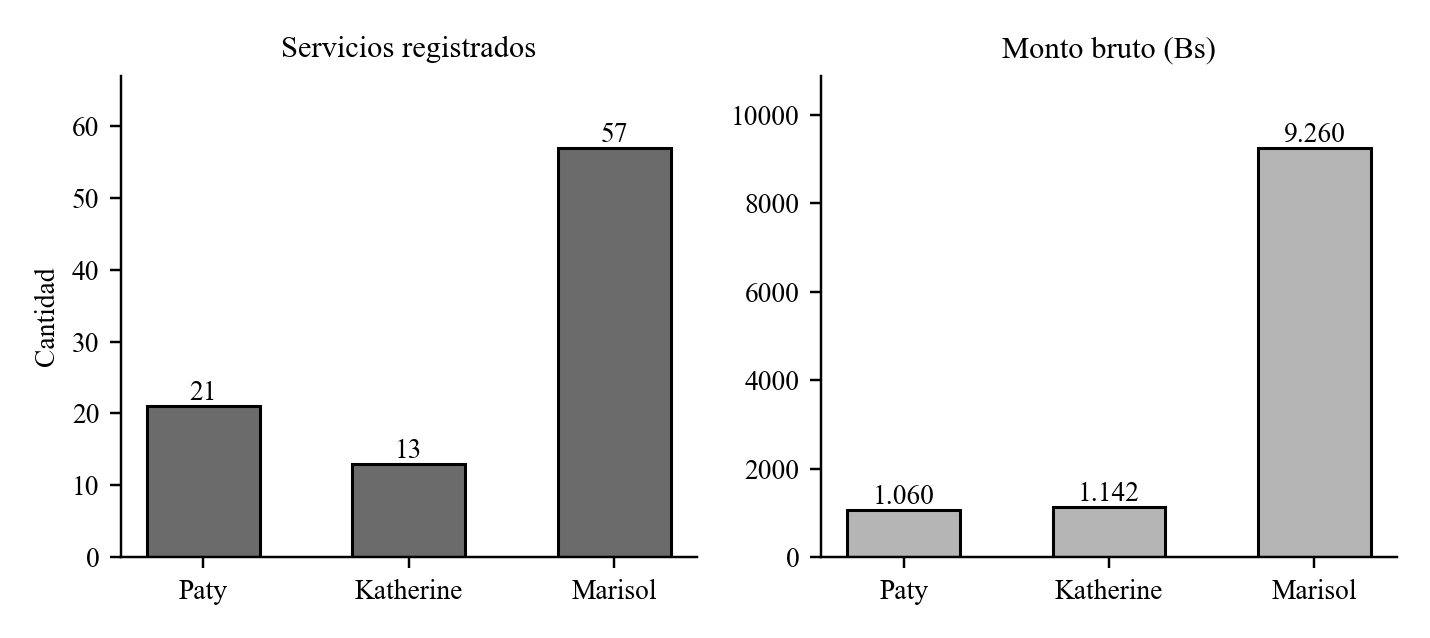
\includegraphics[width=0.9\linewidth]{img/fig_servicios_especialista.png}
\end{figure}
\nota{Elaboración propia a partir de la planilla de pagos de ejemplo (agosto de 2026). Cifras ilustrativas.}

El análisis de la planilla permitió detectar inconsistencias que afectan la confiabilidad de la información (Tabla~\ref{tab:v4_2}). Una de ellas tiene incidencia económica directa: al calcularse la comisión sobre el precio de lista y no sobre el monto cobrado, el salón absorbe íntegramente los descuentos; de haberse aplicado el 35~\% sobre lo cobrado, la comisión total habría sido de Bs~3.513,30, es decir, Bs~498,40 menos. Más allá de la decisión comercial que corresponda, la planilla no permite sostener ni auditar ese criterio.


\vspace{8pt}{\small\setstretch{1.0}
\begin{longtable}{>{\raggedright\arraybackslash}p{0.2195\dimexpr\linewidth-6\tabcolsep\relax}>{\raggedright\arraybackslash}p{0.4269\dimexpr\linewidth-6\tabcolsep\relax}>{\raggedright\arraybackslash}p{0.3536\dimexpr\linewidth-6\tabcolsep\relax}}
\caption{Inconsistencias detectadas en la planilla de ejemplo de agosto de 2026}\label{tab:v4_2}\\
\toprule
\textbf{Hallazgo} & \textbf{Evidencia en la planilla} & \textbf{Consecuencia} \\
\midrule\endfirsthead
\toprule
\textbf{Hallazgo} & \textbf{Evidencia en la planilla} & \textbf{Consecuencia} \\
\midrule\endhead
\bottomrule\endfoot
\bottomrule\endlastfoot
Servicio en texto libre & «PEDI» y « PEDI»; «KAPPING» y «KAPPIN»; «SOFTGEL» y «SOFT GEL» & No es posible totalizar por servicio sin depuración manual \\
Combos sin descomponer & «LIFTING+HENNA+CEJAS»; «MANI+PEDI+TIPS» & El precio no es trazable al catálogo oficial \\
Precios fuera de catálogo & «MANI GEL» cobrado a Bs~112 (catálogo: Bs~120) & Diferencias entre lista y cobro sin motivo registrado \\
Estructura distinta entre hojas & Una hoja sin columna de ganancia neta; propinas en columnas sin nombre; una suma almacenada como texto & Riesgo de errores de suma y de omisión \\
Sin método de pago & No existe la columna & No se puede cuadrar la caja por efectivo, QR o transferencia \\
Sin cancelaciones ni deducciones & No existen columnas para adelantos, faltas o materiales & La liquidación neta queda incompleta \\
Clientes en texto libre & nombres con anotaciones personales (p. ej., relaciones con otras clientas); nombres duplicados con espacios finales & No existe ficha de cliente ni historial \\
\end{longtable}}
\nota{Elaboración propia a partir del análisis de la planilla de pagos de ejemplo (agosto de 2026).}

En consecuencia, el problema se manifiesta en tres planos: la \textbf{exactitud} (riesgo de error en comisiones y totales), la \textbf{eficiencia} (la liquidación semanal exige revisión manual de cada hoja) y la \textbf{trazabilidad} (no se conserva quién modificó un dato ni su valor anterior). A ello se suma la dependencia de una única administradora que registra la información durante la jornada, de pie y, en general, desde el teléfono móvil, una condición para la cual una hoja de cálculo no está diseñada.


\subsection{Delimitación}

\textbf{Espacial:} salón de belleza Lush Beauty, ciudad de Santa Cruz de la Sierra, Bolivia. \textbf{Temporal:} diagnóstico con la planilla de ejemplo de agosto de 2026, línea base retrospectiva y prueba piloto en enero de 2027. \textbf{Poblacional:} la administradora y las especialistas del salón (tres personas) y los registros de servicios generados en el periodo. \textbf{Temática:} gestión de caja y liquidación de comisiones; quedan fuera la agenda de reservas, la facturación electrónica y el inventario.


Adicionalmente, la ampliación hacia el soporte para decisiones establece las siguientes delimitaciones y restricciones:

\begin{vinetas}
\item Ámbito temático: servicios, clientes mínimos, cobros, descuentos, propinas, comisiones, deducciones, cierres, importación, auditoría y reportes.
\item Fuera del MVP: agenda de reservas, facturación electrónica, inventario, reconocimiento visual de uñas, pasarela bancaria automática y aplicación React Native independiente.
\item Restricción metodológica: los datos mensuales representativos no permiten afirmar efectos económicos observados ni justificar modelos predictivos complejos sin historial adicional.
\end{vinetas}

\subsection{Formulación del problema}

\textbf{Pregunta principal:} ¿De qué manera influye la implementación de un sistema web móvil de gestión de caja y nómina en la eficiencia y la exactitud de la liquidación semanal de comisiones del salón Lush Beauty de la ciudad de Santa Cruz de la Sierra durante el periodo noviembre de 2026 – marzo de 2027?


Como ampliación orientada a la toma de decisiones, se formula además la siguiente pregunta complementaria: ¿De qué manera el diseño y uso de un sistema inteligente de soporte para decisiones, basado en registros financieros verificables, simulación de escenarios, comparación multicriterio y recomendaciones explicables, puede contribuir a mejorar la calidad, oportunidad y trazabilidad de las decisiones de caja, precios, descuentos y comisiones del salón Lush Beauty, sin perder eficiencia operativa?

\subsection{Sistematización del problema}

\begin{vinetas}
\item ¿Cómo se realizan actualmente el registro de servicios, el cobro y la liquidación de comisiones en el salón?
\item ¿Qué inconsistencias y riesgos presenta la planilla actual y qué impacto económico tienen?
\item ¿Qué funcionalidades ofrecen los sistemas comerciales similares y qué brechas dejan frente a las necesidades del salón?
\item ¿Qué requisitos, reglas de negocio y arquitectura debe tener un sistema que resuelva estas brechas?
\item ¿En qué medida el sistema reduce el tiempo de liquidación y los errores de cálculo, y qué usabilidad perciben sus usuarias?
\item ¿Qué decisiones financieras y operativas del salón (descuentos, precios, comisiones y cierres de caja) puede apoyar un sistema de soporte basado en simulación de escenarios y comparación multicriterio?
\item ¿Cómo se garantiza que las recomendaciones del sistema sean explicables, trazables y estén siempre sujetas a la aprobación humana?
\end{vinetas}

\section{Objetivos de la Investigación}\label{cap:objetivos}

\subsection{Objetivo general}

Diseñar y validar un sistema web móvil multi-inquilino para la gestión de caja y la liquidación semanal de comisiones del salón de belleza Lush Beauty, con el fin de reducir el tiempo y los errores del proceso actual basado en hojas de cálculo, entre noviembre de 2026 y marzo de 2027.


En su ampliación hacia el soporte para decisiones, el objetivo general se precisa así: diseñar y evaluar como prototipo un Sistema Inteligente de Soporte para la Toma de Decisiones Financieras y Operativas para el salón de belleza Lush Beauty, integrando gestión de caja y nómina, análisis de rentabilidad por servicio, simulación de escenarios, comparación de alternativas y recomendaciones explicables, con el fin de facilitar decisiones informadas y mejorar la trazabilidad de sus fundamentos.

\subsection{Objetivos específicos}

\begin{vinetas}
\item Describir el proceso actual de registro de servicios, cobro y liquidación de comisiones a partir de la planilla de ejemplo de agosto de 2026 y de la entrevista a la administradora.
\item Identificar las inconsistencias y los riesgos de la planilla, cuantificando su impacto en los montos de comisión.
\item Comparar sistemas comerciales similares mediante benchmarking para establecer las brechas funcionales por cubrir.
\item Establecer los requisitos funcionales y no funcionales, el modelo de datos y la arquitectura del sistema propuesto.
\item Evaluar el efecto del sistema sobre el tiempo de liquidación, la tasa de errores de cálculo y la usabilidad percibida respecto de la línea base.
\item Implementar un núcleo transaccional para ventas y pagos con catálogo estructurado, cálculo decimal, reglas versionadas, autorización por rol y auditoría de cambios.
\item Desarrollar una interfaz PWA mobile first capaz de registrar operaciones sin conexión y sincronizarlas sin producir duplicados.
\item Construir un importador de Excel con mapeo de columnas, normalización de nombres, detección de duplicados y previsualización de correcciones.
\item Incorporar Lush Insight, un asistente limitado a consultas financieras aprobadas, con respuestas respaldadas por cifras recuperadas desde la API.
\item Desarrollar Lush Guard con alertas basadas en reglas, y evaluar de forma experimental un detector estadístico o de machine learning si existe volumen suficiente de datos.
\item Automatizar con n8n los avisos de cierre de caja, las entregas seguras de liquidaciones y las notificaciones de operaciones que requieren revisión.
\item Evaluar el MVP mediante pruebas de conciliación, tiempos de tarea, seguridad, sincronización, usabilidad y un recorrido demostrable para la feria.
\item Construir un modelo de contribución económica por servicio, diferenciando ingresos cobrados, comisiones, materiales y costos no incluidos.
\item Implementar un simulador What-If capaz de comparar descuentos, precios, reglas de comisión, costos directos y cantidades hipotéticas de servicios sin alterar transacciones.
\item Desarrollar Lush Decision Studio con alternativas, criterios cuantificables y cualitativos, ponderaciones normalizadas, análisis de sensibilidad y registro de supuestos.
\item Diseñar un motor de recomendaciones prescriptivas que utilice resultados calculados y ofrezca justificaciones, advertencias y aprobación humana.
\item Registrar decisiones, expectativas, responsables y resultados posteriores para comparar lo esperado con lo observado.
\item Evaluar calidad de decisiones mediante precisión de escenarios, tiempo de comparación, comprensión de explicaciones y trazabilidad de la recomendación.
\end{vinetas}

\subsection{Criterios de aceptación globales}

El MVP de la materia deberá ejecutar al menos un caso de decisión completo: registrar o importar datos de prueba, calcular contribución, crear tres escenarios, comparar dos o más alternativas mediante criterios visibles, mostrar la sensibilidad a los pesos, generar una recomendación explicada, registrar una aprobación humana y dejar evidencia de una revisión posterior. Además, se comprobarán exactitud monetaria, permisos, no duplicación offline y procesos n8n sujetos a aprobación.


\section{Justificación}\label{cap:justificacion}

\subsection{Justificación teórica}

El estudio aporta evidencia empírica sobre la aplicación de principios de ingeniería de software y de modelos de evaluación de sistemas de información en el contexto de una microempresa de servicios, un ámbito poco documentado en la literatura regional. Contrasta, con datos del salón, los supuestos sobre errores en hojas de cálculo (Panko, 1998) y sobre la utilidad y la facilidad de uso percibidas como determinantes de la adopción tecnológica (Davis, 1989).


\subsection{Justificación práctica}

El sistema resuelve un problema concreto: reemplazar la planilla por una herramienta que registre servicios contra un catálogo oficial, controle métodos de pago y cancelaciones, y calcule automáticamente la liquidación semanal (comisiones más propinas menos deducciones). La administradora podrá operar desde su teléfono, incluso con conexión intermitente, y obtener reportes en Excel y comprobantes en PDF listos para compartir con su personal.


Las tareas manuales de la administradora se concentran en identificar servicios, comparar montos, cuadrar medios de pago y preparar pagos de personal. Un flujo único reduce la necesidad de copiar información entre hojas y facilita identificar diferencias antes de cerrar una semana. El simulador de políticas permite conocer el efecto de escenarios sin convertir la sugerencia de un algoritmo en una decisión salarial automática. Su valor económico debe determinarse con mediciones reales del tiempo de trabajo y de las discrepancias, no mediante ahorros supuestos.


\subsection{Justificación metodológica}

La investigación propone un procedimiento replicable para evaluar sistemas de gestión en microempresas con muestras pequeñas: línea base documental, pruebas de conciliación contra un cálculo de referencia, registro cronometrado de tiempos y cuestionario estandarizado de usabilidad (Brooke, 1996). Los instrumentos pueden reutilizarse en otros salones.


\subsection{Justificación social}

Beneficia a un emprendimiento liderado por mujeres y a sus especialistas, quienes recibirán liquidaciones transparentes, verificables y con detalle línea a línea. A mediano plazo, la arquitectura multi-inquilino permite ofrecer la solución a otros salones y pequeños negocios, fortaleciendo la formalización de su gestión financiera.


La propuesta mantiene la comparación de una línea base con un piloto y el uso de instrumentos de observación y usabilidad. También protege la confidencialidad de la nómina de cada especialista y permite explicar cada liquidación línea por línea. Al ofrecer herramientas comprensibles para un negocio de pequeña escala, puede apoyar una gestión más transparente; esta posibilidad debe demostrarse empíricamente durante el piloto.


\subsection{Justificación tecnológica}

El monolito modular conserva la simplicidad operativa del sistema y separa responsabilidades críticas. React y TypeScript permiten una experiencia consistente en escritorio y teléfono; Django REST Framework centraliza las reglas; PostgreSQL facilita integridad transaccional y trazabilidad; IndexedDB conserva registros pendientes; n8n ejecuta comunicaciones desacopladas. Esta combinación prioriza demostrabilidad, mantenimiento y control por encima de la adopción de microservicios sin necesidad comprobada.


\subsection{Justificación de innovación}

El elemento distintivo no es la mera presencia de un chatbot o de machine learning. La innovación funcional está en enlazar, dentro de una operación pequeña, conciliación financiera, recuperación de datos de Excel y explicaciones de situaciones económicas con evidencia de origen. La importación inteligente se apoya primero en reglas y similitud textual; el análisis conversacional consulta funciones cerradas del backend; las alertas señalan hechos verificables. Se minimiza así el riesgo de respuestas atractivas pero financieramente incorrectas.


\section{Marco Teórico}\label{cap:marco}

El marco teórico reúne los antecedentes y los fundamentos conceptuales que sustentan el estudio: los sistemas de información para el registro de transacciones, la ingeniería de requisitos, la calidad del producto, los errores en hojas de cálculo, las arquitecturas multi-inquilino, el diseño móvil primero y los modelos de éxito y aceptación de los sistemas. Su propósito es justificar por qué las variables seleccionadas (eficiencia, exactitud y usabilidad) son adecuadas para evaluar la propuesta, y cómo cada fundamento se traduce en requisitos concretos del sistema. Además, se incorporan los fundamentos tecnológicos y de decisión de la ampliación Lush Beauty Smart DSS: las transacciones atómicas, el funcionamiento sin conexión, la inteligencia artificial con herramientas restringidas, la detección de anomalías, la automatización con n8n, los sistemas de soporte para decisiones, el análisis de escenarios What-If y el análisis multicriterio.

\subsection{Antecedentes de la investigación}

\subsubsection{Estudios sobre errores en hojas de cálculo}

Panko (1998) sintetizó los hallazgos de auditorías realizadas sobre hojas de cálculo en uso y concluyó que los errores son frecuentes y difíciles de detectar para quien construyó el archivo. Su trabajo es el antecedente más directo del problema de Lush Beauty, porque la planilla de comisiones del salón es una hoja de cálculo de uso operativo: contiene fórmulas repetidas en cada hoja, datos digitados a mano y ningún mecanismo de validación. El argumento de Panko sustenta la decisión de calcular las comisiones en un servidor y no en la planilla de cada persona.


\subsubsection{Sistemas web para la gestión de salones de belleza}

Ochoa López (2021), en una propuesta tecnológica de la Universidad Agraria del Ecuador, desarrolló un sistema web para administrar los procesos de una peluquería y de un salón de estética en Milagro, Ecuador, implementado en Python. El documento consultado permitió verificar su alcance a partir de la portada y del índice; el contenido completo debe revisarse para confirmar si incluye cálculo de comisiones, caja y liquidación de personal. Su pertinencia radica en que aborda el mismo problema de gestión administrativa en un salón de tamaño comparable.


Meré Espino (2016), en un proyecto fin de carrera de la Universidad de Las Palmas de Gran Canaria, propuso un sitio web para un negocio de tratamientos de belleza con un área privada para gestionar la agenda, enviar publicidad y citar a los clientes. Según el resumen del repositorio, el énfasis está en la presencia en línea y en la agenda, no en la caja ni en la liquidación del personal, lo que lo distingue del problema que aborda este estudio.


\subsubsection{Vacío identificado}

Los antecedentes revisados se concentran en la agenda, las citas y la presencia web de los salones. Ninguno de los consultados trata de forma explícita la liquidación semanal de comisiones con deducciones, excedentes y propinas, ni el cuadre de caja por método de pago. Tampoco se localizaron trabajos bolivianos verificables sobre el tema en los repositorios consultados; esa búsqueda debe completarse en los repositorios de universidades bolivianas durante la revisión bibliográfica. Esta brecha justifica un sistema que prioriza la caja y la nómina, y deja la agenda para una etapa posterior. Los sistemas comerciales se analizan en el Capítulo~\ref{cap:benchmarking}.


\subsection{Bases teóricas}

\subsubsection{Sistemas de información y procesamiento de transacciones}

Laudon y Laudon (2016) definen un sistema de información como un conjunto de componentes interrelacionados que captan, procesan, almacenan y distribuyen información para apoyar la toma de decisiones y el control de una organización. Dentro de esta categoría, los sistemas de procesamiento de transacciones registran las operaciones cotidianas y alimentan a los demás niveles de información; de su exactitud depende la calidad de los reportes y de las decisiones que se derivan de ellos.


En el salón, cada servicio prestado constituye una transacción que contiene fecha, especialista, servicio, precio, descuento, método de pago y, cuando corresponde, propina. Esa transacción alimenta tres procesos: el cuadre de la caja diaria, el cálculo de la comisión y la liquidación semanal. Por ello, el sistema debe garantizar que cada transacción se registre una sola vez, con la hora asignada por el servidor y con la regla de cálculo vigente en el momento de la venta.


\subsubsection{Ingeniería de requisitos y técnicas de obtención}

Sommerville (2011) describe la ingeniería de requisitos como un proceso que comprende la obtención, el análisis, la especificación y la validación de lo que un sistema debe hacer y de las restricciones bajo las que debe operar. Distingue entre requisitos funcionales, que describen los servicios que el sistema debe prestar, y requisitos no funcionales, que fijan propiedades como el desempeño, la seguridad o la facilidad de uso.


Entre las técnicas de obtención, el mismo autor destaca las entrevistas, los cuestionarios, la observación del trabajo real y el análisis de documentos existentes. En este estudio, la planilla de ejemplo funciona como documento de análisis, la observación cronometrada mide el trabajo real y el cuestionario de requerimientos (Anexo A) recoge, de forma estructurada y comparable, las necesidades de la administradora y de las especialistas en los módulos de registro de servicios, comisiones, propinas, deducciones, clientes, importación y uso. La priorización con una escala de importancia permite separar lo imprescindible para el producto mínimo viable de lo que corresponde a etapas posteriores.


\subsubsection{Calidad del producto y calidad en uso}

La norma ISO/IEC 25010 (International Organization for Standardization [ISO] \& International Electrotechnical Commission [IEC], 2011) define un modelo de calidad del producto con ocho características: adecuación funcional, eficiencia de desempeño, compatibilidad, usabilidad, fiabilidad, seguridad, mantenibilidad y portabilidad. Complementa ese modelo con un modelo de calidad en uso, que evalúa la efectividad, la eficiencia, la satisfacción, la libertad frente al riesgo y la cobertura del contexto de uso.


Para esta investigación, la adecuación funcional corresponde a la exactitud de los cálculos, la eficiencia de desempeño al tiempo de registro y de liquidación, y la usabilidad a la facilidad con que la especialista completa un registro. Estos vínculos explican la elección de los indicadores de la operacionalización (Capítulo~\ref{cap:operacionalizacion}).


La calidad debe evaluarse tanto por exactitud funcional como por la facilidad de uso y la seguridad de los datos. Se mantienen los indicadores de tiempo de liquidación, tasa de discrepancias y cuestionario SUS descritos en la operacionalización de las variables, complementados con pruebas de sincronización offline, aislamiento por salón y verificación de permisos. Debido a la muestra pequeña prevista, la interpretación se centrará en resultados descriptivos y evidencia reproducible, evitando afirmaciones generales no respaldadas.

\subsubsection{Errores en hojas de cálculo y control de cálculos}

Panko (1998) clasifica los errores de las hojas de cálculo en mecánicos (fórmulas mal escritas o referencias equivocadas), lógicos (reglas de negocio aplicadas de forma incorrecta) y de omisión (datos o filas que faltan). Advierte, además, que la revisión realizada por la misma persona que elaboró el archivo detecta solo una parte de ellos.


Esta clasificación orienta los controles del sistema propuesto. Los errores mecánicos se evitan con un motor de cálculo único en el servidor; los lógicos, con reglas de comisión configurables y con vigencia; y los de omisión, con validaciones de entrada y con un cuadre de control entre pagos, líneas y liquidaciones. Los cálculos monetarios se realizan con tipos decimales, y cada línea conserva una copia (\textit{snapshot}) de la regla y del precio aplicados, de modo que un cambio posterior no altere el pasado.


En un sistema transaccional, cada servicio prestado origina un registro identificable y, cuando corresponde, uno o varios pagos. La suma de pagos debe corresponder al importe exigible; el cálculo de comisión debe aplicar la regla vigente en la fecha de la operación; y cualquier corrección debe quedar ligada a un motivo y a un usuario. El trabajo de Panko (1998) sobre errores en hojas de cálculo fundamenta la necesidad de validaciones y de un cálculo centralizado, mientras que la documentación de Django describe los mecanismos de transacción atómica que permiten confirmar o revertir operaciones compuestas (Django Software Foundation, s. f.-a).

\subsubsection{Arquitectura multi-inquilino}

Una arquitectura multi-inquilino (multi-tenant) es aquella en la que una misma instancia de la aplicación atiende a varios clientes —en este caso, salones— manteniendo sus datos aislados entre sí (Bezemer \& Zaidman, 2010). Aunque el estudio se centra en un único salón, el sistema incorpora desde su diseño un identificador de inquilino en cada entidad y un aislamiento por fila en la base de datos, de modo que la solución pueda ofrecerse más adelante a otros negocios sin reescribir el modelo de datos y sin que la información de un salón sea visible para otro. Esta decisión protege la confidencialidad de los sueldos y de las clientas, y se verifica mediante pruebas de aislamiento, no solo con la presencia del identificador.

\subsubsection{Diseño móvil primero y aplicaciones web progresivas}

El enfoque \textit{mobile first} propone diseñar primero para pantallas pequeñas y contextos de uso restringidos, y ampliar después hacia pantallas mayores. Wroblewski (2011) sostiene que esta restricción obliga a priorizar el contenido y las acciones esenciales, lo que produce interfaces más claras también en el escritorio.


Una aplicación web progresiva (PWA) es un sitio web que puede instalarse en la pantalla de inicio del teléfono y que, mediante técnicas de almacenamiento local y de trabajo en segundo plano, puede seguir operando de forma parcial sin conexión. En el sistema propuesto, la PWA permite registrar servicios aunque falle la red del salón: cada registro queda en una cola local, se identifica con una clave única para que su reenvío no duplique la venta, y se sincroniza al recuperar la conexión. Estas decisiones responden al uso real de la administradora, que registra desde el teléfono durante la jornada.


El enfoque mobile first diseña primero la acción cotidiana de registro con el menor número de pasos. Una aplicación web progresiva puede instalarse en el dispositivo y utilizar Service Workers e IndexedDB para mantener recursos e información durante interrupciones. No obstante, no debe suponerse que todos los navegadores ejecutan sincronizaciones en segundo plano de la misma manera; el producto incorporará reintentos al reabrir la aplicación o recuperar la conexión, además de un indicador visible de registros pendientes (Mozilla Developer Network [MDN], s. f.-a).

\subsubsection{Modelos de éxito y aceptación de sistemas de información}

DeLone y McLean (2003) propusieron un modelo de éxito de los sistemas de información que integra seis dimensiones: calidad del sistema, calidad de la información, calidad del servicio, uso, satisfacción del usuario y beneficios netos. El modelo permite evaluar un sistema más allá de su funcionamiento técnico, al considerar el uso que se le da y el beneficio que produce para la organización.


Davis (1989), por su parte, demostró que la utilidad percibida y la facilidad de uso percibida predicen la intención de usar una tecnología. Ambos modelos orientan los indicadores del estudio: la utilidad se traduce en la reducción del tiempo de liquidación y de los errores; la facilidad de uso, en la puntuación de usabilidad; y la satisfacción y el uso continuado, en las entrevistas de seguimiento durante el piloto.


\subsubsection{Inteligencia artificial generativa con herramientas restringidas}

Un modelo de lenguaje es adecuado para traducir una pregunta de gestión a una consulta permitida y redactar un resumen comprensible, siempre que no sea la fuente de verdad financiera. Lush Insight expondrá herramientas tipadas, como consultar\_resumen\_caja(periodo) o consultar\_impacto\_descuentos(periodo), cuyas respuestas provendrán de cálculos del backend. El modelo no tendrá credenciales de escritura ni acceso directo a tablas completas de salarios y clientes. Toda respuesta incluirá período, magnitudes, alcance y advertencia cuando no existan datos suficientes.

\subsubsection{Detección de anomalías y machine learning}

La detección de anomalías busca identificar casos poco habituales con respecto a una distribución o una política. Para una base pequeña es preferible comenzar con reglas interpretables: descuentos superiores al umbral autorizado, ventas sin medio de pago, diferencias de caja, ediciones repetidas o precios fuera de catálogo. Isolation Forest, disponible en scikit-learn, constituye una alternativa experimental cuando el volumen y la calidad del historial sean adecuados; su salida representa atipicidad estadística, nunca prueba de fraude (scikit-learn Developers, s. f.-a).

\subsubsection{Automatización mediante n8n}

n8n permite conectar servicios mediante disparadores, condiciones y acciones. En Lush Beauty Smart se reservará para trabajos posteriores al registro contable, como generar avisos, distribuir comprobantes y solicitar revisiones. El backend publicará eventos autenticados que describan una acción ya aprobada. El flujo automatizado deberá incorporar control de duplicados, reintentos, límites de exposición de información y registros de ejecución. El cálculo de nómina no dependerá de un nodo de automatización (n8n, s. f.).

\subsubsection{Sistemas de soporte para decisiones (DSS)}\label{sec:dss}

Un sistema de soporte para decisiones integra datos, modelos analíticos y una interfaz de interacción para ayudar a una persona a evaluar problemas semiestructurados. En Lush Beauty Smart DSS, la base de datos proporciona hechos transaccionales; el componente de modelos produce escenarios, medidas de contribución y comparaciones; y la administradora aporta objetivos, límites y preferencias. El sistema no sustituye la responsabilidad de decidir.

\subsubsection{Análisis de escenarios What-If y sensibilidad}

La simulación What-If modifica supuestos controlados para estimar el efecto de una alternativa. Se deben identificar variables independientes (precio, descuento, demanda hipotética, comisión y materiales), reglas de negocio fijas, variables de salida y restricciones. El análisis de sensibilidad repite la comparación con diferentes supuestos para evaluar si una recomendación es estable o depende de una hipótesis frágil.

\subsubsection{Análisis multicriterio y recomendaciones prescriptivas}

Cuando una decisión incorpora resultados económicos, liquidez, dificultad operativa y riesgo, no basta elegir el mayor ingreso. Una matriz de puntuación ponderada constituye un primer instrumento exploratorio; debe documentar quién asigna pesos, cómo se normalizan las escalas y qué sucede cuando estos cambian. Una evaluación multicriterio completa requiere analizar compensaciones y sensibilidad de forma explícita, evitando presentar una puntuación simple como verdad objetiva (HM Treasury, s. f.).

\subsubsection{Evaluación de artefactos y calidad de la explicación}

La investigación de diseño construye y evalúa soluciones tecnológicas frente a problemas relevantes (Hevner et al., 2004). Para este DSS no alcanza medir si el software calcula: también importa si las alternativas son comprensibles, las recomendaciones son reproducibles y el usuario conserva control. Los principios de gestión de riesgos de IA de NIST (2023) respaldan documentar límites, validez y supervisión humana.

\subsection{Definición de términos clave}

\noindent \textbf{Análisis de sensibilidad.} Repetición de una comparación con distintos supuestos o pesos para evaluar si una recomendación es estable o depende de una hipótesis frágil.

\noindent \textbf{Backoffice.} Módulo administrativo interno del negocio, no visible para el cliente final.

\noindent \textbf{Benchmarking.} Proceso sistemático de comparar productos, procesos o prácticas con los de referentes del sector para identificar oportunidades de mejora.

\noindent \textbf{Bitácora de auditoría.} Registro de solo inserción en el que se guardan las acciones realizadas en el sistema, con usuario, fecha, valor anterior y valor nuevo.

\noindent \textbf{Cola de sincronización.} Conjunto de registros guardados en el dispositivo mientras no hay conexión, que se envían al servidor cuando la conexión se restablece.

\noindent \textbf{Comisión.} Porción del precio de un servicio que corresponde a la especialista que lo realiza. En el caso de estudio, equivale al 35~\% del precio de lista como valor inicial de la regla.

\noindent \textbf{Contribución por servicio.} Precio realmente cobrado menos la comisión reconocida y los costos variables directos del servicio; no equivale a la utilidad neta del negocio.

\noindent \textbf{DSS (sistema de soporte para decisiones).} Sistema que integra datos, modelos analíticos y una interfaz de interacción para ayudar a una persona a evaluar problemas semiestructurados; no sustituye la responsabilidad de decidir.

\noindent \textbf{Escenario What-If.} Simulación que modifica supuestos controlados (precio, descuento, comisión, costos, cantidad) para estimar el efecto de una alternativa sin alterar los registros reales.

\noindent \textbf{Excedente de deducción.} Monto de deducciones que supera lo ganado en un periodo y que se descuenta en la liquidación siguiente, identificado como tal en los reportes.

\noindent \textbf{Idempotencia.} Propiedad de una operación que, repetida con la misma clave, produce un solo resultado; evita duplicar ventas en reintentos de red.

\noindent \textbf{IndexedDB.} Almacén local del navegador para datos estructurados y cola de trabajo.

\noindent \textbf{Isolation Forest.} Algoritmo no supervisado para detectar valores estadísticamente atípicos.

\noindent \textbf{Liquidación.} Cálculo periódico del monto neto a pagar a una trabajadora: sueldo fijo más comisiones y propinas, menos deducciones.

\noindent \textbf{LLM.} Modelo de lenguaje que ayuda a interpretar preguntas y redactar respuestas.

\noindent \textbf{Matriz ponderada.} Instrumento exploratorio de análisis multicriterio que suma puntuaciones normalizadas de cada alternativa según criterios con pesos explícitos.

\noindent \textbf{Multi-inquilino.} Arquitectura en la que una misma aplicación atiende a varios negocios con datos aislados entre sí.

\noindent \textbf{Outbox.} Tabla de eventos por enviar que se crea junto con la transacción principal.

\noindent \textbf{PWA.} Aplicación web progresiva instalable en el teléfono que puede operar parcialmente sin conexión.

\noindent \textbf{Requisito funcional.} Descripción de un servicio o comportamiento que el sistema debe ofrecer, por ejemplo, calcular la comisión de una línea de venta.

\noindent \textbf{Requisito no funcional.} Restricción de calidad o de operación, como el tiempo de respuesta, la seguridad o la facilidad de uso.

\noindent \textbf{Seguridad a nivel de fila (RLS).} Mecanismo de la base de datos que limita las filas visibles para cada sesión según una condición; en este caso, el inquilino.

\noindent \textbf{Snapshot.} Copia de los valores vigentes en el momento de una transacción (precio y regla de comisión) que no cambia cuando se modifican los valores originales.

\noindent \textbf{Tasa de error.} Proporción de líneas o liquidaciones cuyo resultado difiere del cálculo de referencia.

\noindent \textbf{Tool calling.} Invocación de herramientas predeterminadas desde un asistente de lenguaje.

\subsection{Relación entre los fundamentos teóricos y los requisitos del sistema}

Los fundamentos anteriores se traducen en requisitos concretos. La correspondencia siguiente permite verificar que ninguna necesidad del salón quede sin sustento teórico y que ningún requisito quede sin justificación.


\begin{vinetas}
\item \textbf{Procesamiento de transacciones} (Laudon \& Laudon, 2016): cada servicio es una transacción con fecha, especialista y pago; requiere registro con fecha y hora automáticas y cobro único.
\item \textbf{Requisitos funcionales y no funcionales} (Sommerville, 2011): las reglas de comisión son funcionales; el tiempo de respuesta y la facilidad de uso son no funcionales. Ambos se obtienen con el cuestionario de requerimientos.
\item \textbf{Calidad del producto y en uso} (ISO/IEC, 2011): la exactitud, la eficiencia y la usabilidad se convierten en los indicadores de la operacionalización.
\item \textbf{Errores en hojas de cálculo} (Panko, 1998): los errores mecánicos, lógicos y de omisión motivan el cálculo en servidor, las validaciones y la bitácora de cambios.
\item \textbf{Arquitectura multi-inquilino} (Bezemer \& Zaidman, 2010): el identificador de inquilino y el aislamiento por fila protegen los datos de cada salón.
\item \textbf{Diseño móvil primero y PWA} (Wroblewski, 2011): el flujo de registro se diseña para pocos toques y el registro funciona sin conexión.
\item \textbf{Éxito y aceptación} (DeLone \& McLean, 2003; Davis, 1989): el uso, la satisfacción y la utilidad percibida se miden en el piloto.
\item Transacciones atómicas y exactitud financiera (Django Software Foundation, s. f.-a): las operaciones compuestas se confirman o se revierten por completo, lo que sustenta el cierre de caja, la liquidación y la importación en transacciones controladas.
\item Funcionamiento sin conexión (Mozilla Developer Network [MDN], s. f.-a): la cola local, la clave de idempotencia y el indicador de registros pendientes responden a las limitaciones de la sincronización en segundo plano de los navegadores.
\item Inteligencia artificial con herramientas restringidas y detección de anomalías: Lush Insight consulta funciones cerradas del backend y Lush Guard comienza con reglas interpretables; el aprendizaje automático queda como experimento hasta contar con historial suficiente.
\item Sistemas de soporte para decisiones, análisis What-If y multicriterio (HM Treasury, s. f.): la contribución por servicio, los escenarios, la matriz ponderada y la sensibilidad convierten los datos transaccionales en alternativas comparables, siempre con aprobación humana.
\item Evaluación de artefactos y gestión de riesgos de IA (Hevner et al., 2004; National Institute of Standards and Technology [NIST], 2023): se documentan límites, validez y supervisión humana de las recomendaciones.
\end{vinetas}

\section{Benchmarking de Sistemas Similares}\label{cap:benchmarking}

El benchmarking, entendido como la búsqueda de las mejores prácticas que conducen a un desempeño superior (Camp, 1989), se aplicó para comparar el sistema propuesto con cuatro plataformas comerciales de gestión de salones —Fresha, Booksy, AgendaPro y Vagaro— y con la solución actualmente usada por el salón (hoja de cálculo). La selección se basó en su presencia en el mercado hispanohablante o internacional y en que ofrecen funciones de agenda, cobro y comisiones. La información proviene de las páginas oficiales de cada producto, consultadas el 30 de octubre de 2026.


Los criterios de comparación derivan de las necesidades del salón: comisiones configurables, propinas, liquidación de personal, importación desde Excel, funcionamiento sin conexión y modelo de costo. La Tabla~\ref{tab:v4_3} resume los resultados. La expresión «No documentado» indica que la página consultada no menciona la función, lo que no implica necesariamente que el producto carezca de ella.


\vspace{8pt}{\footnotesize\setstretch{1.0}
\begin{longtable}{>{\raggedright\arraybackslash}p{0.1573\dimexpr\linewidth-14\tabcolsep\relax}>{\raggedright\arraybackslash}p{0.1331\dimexpr\linewidth-14\tabcolsep\relax}>{\raggedright\arraybackslash}p{0.1411\dimexpr\linewidth-14\tabcolsep\relax}>{\raggedright\arraybackslash}p{0.1371\dimexpr\linewidth-14\tabcolsep\relax}>{\raggedright\arraybackslash}p{0.1411\dimexpr\linewidth-14\tabcolsep\relax}>{\raggedright\arraybackslash}p{0.1371\dimexpr\linewidth-14\tabcolsep\relax}>{\raggedright\arraybackslash}p{0.1532\dimexpr\linewidth-14\tabcolsep\relax}}
\caption{Comparación de sistemas de gestión para salones de belleza}\label{tab:v4_3}\\
\toprule
\textbf{Criterio} & \textbf{Fresha} & \textbf{Booksy} & \textbf{AgendaPro} & \textbf{Vagaro} & \textbf{Hoja de cálculo (actual)} & \textbf{Lush Beauty (propuesta)} \\
\midrule\endfirsthead
\toprule
\textbf{Criterio} & \textbf{Fresha} & \textbf{Booksy} & \textbf{AgendaPro} & \textbf{Vagaro} & \textbf{Hoja de cálculo (actual)} & \textbf{Lush Beauty (propuesta)} \\
\midrule\endhead
\bottomrule\endfoot
\bottomrule\endlastfoot
Agenda y reservas en línea & Sí & Sí & Sí & Sí & No & Fuera del MVP (futuro) \\
Punto de venta y cierre de caja & Sí & Sí (con procesador de pagos) & Parcial (cierres de caja) & Sí (terminales propias) & Manual & Sí; caja diaria por método de pago \\
Comisiones del personal & No documentado & Sí, automática en cada cobro & Sí, mediante reporte & No documentado & Fórmula fija 35~\% por hoja & Sí; reglas configurables con vigencia \\
Propinas & Parcial (se cobran en la reserva) & Sí, seguimiento automático & No documentado & No documentado & Columna aparte & Sí; ajustables y con política de reparto \\
Liquidación de nómina & No documentado & Parcial (cálculo de comisiones y propinas) & No documentado & No documentado & Manual & Sí; semanal, con deducciones y excedente \\
Importación desde Excel & Parcial (clientes e inventario) & No documentado & No documentado & No documentado & No aplica & Sí; vista previa y detección de duplicados \\
Uso sin conexión & No documentado & No documentado & No documentado & No documentado & Sí (archivo local) & Sí; cola local y sincronización \\
Auditoría de cambios & No documentado & No documentado & No documentado & No documentado & No & Sí; bitácora inmutable \\
Modelo de costo & Suscripción mensual con complementos & USD 29,99 al mes más USD 20 por usuario adicional & Planes por suscripción (precios no visibles) & Suscripción mensual (USD 23,99) más comisión de procesamiento & Sin costo adicional & Desarrollo propio; costo de alojamiento \\
\end{longtable}}
\nota{Elaboración propia a partir de las páginas oficiales de Fresha (s. f.), Booksy (s. f.), AgendaPro (s. f.) y Vagaro (s. f.), consultadas el 30 de octubre de 2026. Los precios son referenciales y están sujetos a cambios.}

De la comparación se desprenden tres conclusiones. Primero, las plataformas comerciales priorizan la agenda y el cobro con tarjeta, y tratan la liquidación de personal de forma parcial: la mayoría documenta el cálculo de comisiones, pero no un proceso de liquidación periódica con deducciones. Segundo, ninguna de las páginas consultadas describe la importación de planillas heredadas de un salón ni el registro sin conexión, dos requisitos críticos para una microempresa que opera desde el teléfono y que migra desde Excel. Tercero, el modelo de costo en dólares y por usuario adicional puede resultar oneroso para un salón de tres personas, además de que las reglas de comisión propias del negocio (porcentaje sobre precio de lista, excedente de deducción) no son parametrizables en el grado requerido.


Estas brechas justifican el desarrollo de una solución propia, enfocada en caja y nómina, que incorpore lo que las plataformas comerciales ya resolvieron bien —cobro, comisiones automáticas, aplicación móvil— y cubra lo no documentado en ellas. La agenda de reservas se incorporará en una etapa posterior, aprovechando que el catálogo se expondrá mediante una interfaz de consulta pública.


La Figura~\ref{fig:v4_2} muestra la arquitectura propuesta: una aplicación cliente instalable, una interfaz de programación (API) con módulos de dominio y una base de datos relacional con aislamiento por inquilino y bitácora inmutable.


\begin{figure}[H]
\caption{Arquitectura propuesta del sistema Lush Beauty}\label{fig:v4_2}
\centering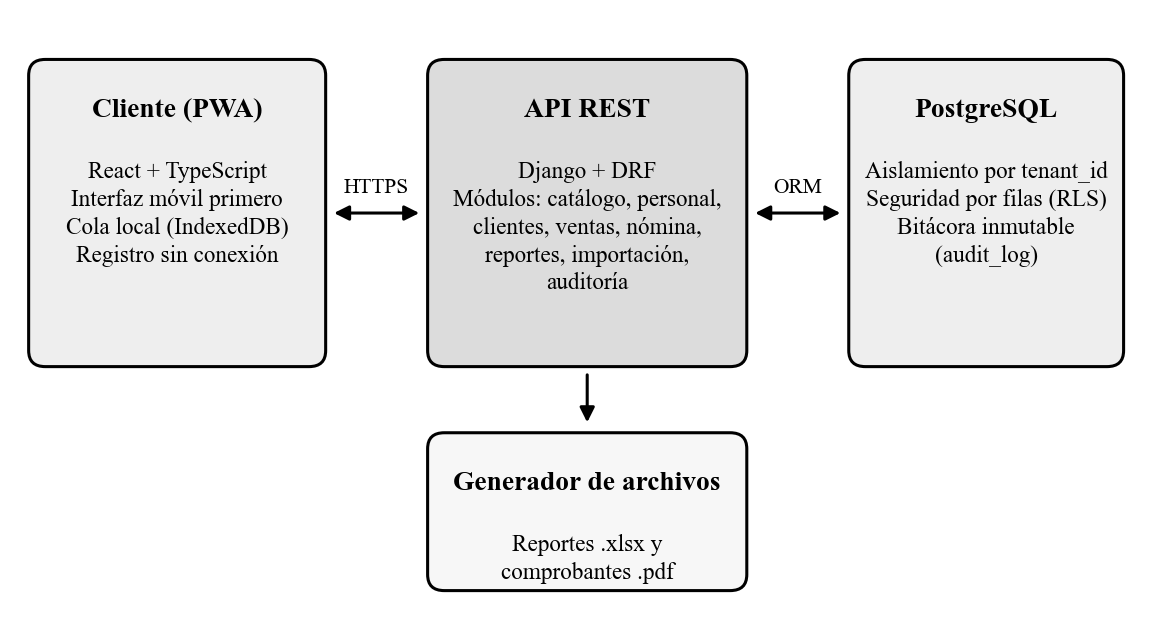
\includegraphics[width=0.9\linewidth]{img/fig_arquitectura_v4.png}
\end{figure}
\nota{Elaboración propia. PWA: aplicación web progresiva; RLS: seguridad a nivel de fila.}

\subsection{Comparación por problema y enfoque}

Para precisar la diferenciación, la Tabla~\ref{tab:dss_3} contrasta cada necesidad del salón con el enfoque de Lush Beauty Smart. La ausencia de una función en la documentación consultada de las plataformas comerciales no demuestra que el proveedor carezca de ella; el contraste se limita a cómo la propuesta prioriza necesidades específicas del negocio.

\vspace{8pt}{\small\setstretch{1.0}
\begin{longtable}{>{\raggedright\arraybackslash}p{0.3333\dimexpr\linewidth-6\tabcolsep\relax}>{\raggedright\arraybackslash}p{0.3333\dimexpr\linewidth-6\tabcolsep\relax}>{\raggedright\arraybackslash}p{0.3333\dimexpr\linewidth-6\tabcolsep\relax}}
\caption{Comparación por problema y enfoque}\label{tab:dss_3}\\
\toprule
\textbf{Criterio} & \textbf{Necesidad de Lush Beauty} & \textbf{Enfoque de la propuesta} \\
\midrule\endfirsthead
\toprule
\textbf{Criterio} & \textbf{Necesidad de Lush Beauty} & \textbf{Enfoque de la propuesta} \\
\midrule\endhead
\bottomrule\endfoot
\bottomrule\endlastfoot
Liquidación semanal & Comisión, propinas y deducciones & Motor versionado y detalle por línea \\
Conciliación & Efectivo, QR y transferencias & Cierre diario con conciliación \\
Migración de Excel & Nombres inconsistentes y columnas dispares & Previsualización y validación asistida \\
Uso móvil sin conexión & Registro durante la atención & PWA con cola idempotente \\
Asistencia financiera & Interpretar causas de variaciones & Lush Insight con consultas permitidas \\
Automatización & Entrega de reportes y alertas & Flujos n8n con eventos aprobados \\
\end{longtable}}
\nota{Elaboración propia. No implica ausencia de estas capacidades en productos comerciales.}

\subsection{Propuesta de valor}

Lush Beauty Smart se posiciona como una plataforma especializada en el flujo financiero de pequeñas empresas de belleza. Su diferenciación propuesta se resume en registrar con rapidez, calcular con exactitud, explicar con evidencia y automatizar sin perder control. La posibilidad de operar múltiples salones mediante aislamiento de datos constituye una opción de expansión futura y no una característica que sea necesario comercializar o probar a escala durante la feria.


\subsection{Diferenciación como sistema de soporte para decisiones}

La comparación comercial realizada en el benchmarking se centra en agenda, caja, comisiones, propinas y reportes. La ampliación DSS no afirma que los productos comparados carezcan de funciones avanzadas: propone una diferenciación evaluable para el caso de estudio, consistente en simular alternativas económicas con reglas visibles y evaluar después los resultados de las decisiones. El benchmarking de estas nuevas capacidades requerirá una verificación específica si se utiliza para afirmar superioridad de mercado.


\section{Propuesta funcional: Lush Beauty Smart}\label{cap:propuesta}

Este capítulo describe la propuesta funcional Lush Beauty Smart, que conserva el núcleo de caja y nómina planteado en el diagnóstico y le añade importación asistida de planillas, asistencia financiera explicable, alertas y automatizaciones controladas. Las funciones se presentan como propuesta de diseño y no como resultados medidos.

\subsection{Usuarios y roles}

Se reconocen tres roles funcionales. La administradora configura catálogo, reglas, descuentos autorizados, cierres y liquidaciones; la especialista registra servicios y consulta exclusivamente el detalle que le corresponde; y el contador o lector de reportes, si es habilitado, accede a informes agregados o exportaciones autorizadas. Una misma persona puede cumplir más de un rol, conservándose los permisos por operación y el historial de sus acciones.


\subsection{Módulo de caja y nómina}

El núcleo financiero incluye catálogo de servicios, agrupaciones de combos, ventas con una o varias líneas, pagos por medio, propinas, descuentos motivados, cancelaciones, reglas de comisión con fecha de vigencia y deducciones de nómina. El cierre registra importe esperado, importe declarado, diferencias y justificación. La liquidación semanal se genera como borrador, se verifica y se aprueba; únicamente después se emite el comprobante definitivo y se habilitan automatizaciones.


\subsubsection{Política de cálculo y conservación de evidencia}

La comisión se calcula por línea aplicando a la base definida el porcentaje vigente en el momento de registrar la venta. Para el caso ilustrativo, la base inicial es el precio de lista y la tasa es 35~\%. La venta guarda una copia inmutable del precio de lista, descuento, importe cobrado, tasa y política aplicada. Un cambio posterior de catálogo o porcentaje no recalcula operaciones históricas. Las devoluciones y anulaciones generan ajustes trazables en vez de eliminar filas utilizadas en una liquidación.


\subsection{Centro de inteligencia financiera}

El panel presenta ventas brutas, netas, descuentos, comisiones estimadas, propinas, pagos por método y cierres pendientes. Permite filtrar por período, especialista y servicio, distinguiendo importes realmente cobrados de registros no confirmados. Un simulador calcula escenarios de comisión sobre precio de lista o importe neto, sin afectar las liquidaciones aprobadas. Las recomendaciones de política se presentan como comparaciones numéricas, no como órdenes de reducir pagos.


\subsection{Importador inteligente de planillas}

El usuario carga un archivo .xlsx; el sistema identifica hojas y columnas, ofrece el mapeo de datos y presenta una vista previa. Una capa de normalización elimina espacios redundantes, unifica mayúsculas y consulta aliases conocidos. Si persisten dudas, una similitud textual como RapidFuzz ordena alternativas por cercanía; los casos por debajo de un umbral conservador quedan pendientes de revisión. Un LLM puede proponerse como recurso opcional de interpretación, sin aceptar cambios automáticamente.


Los combos conocidos se descomponen usando reglas explícitas del catálogo. Cada registro importado conserva la fuente, hoja, número de fila, propuesta de corrección y decisión final. Los registros con información financiera incompleta no se integran silenciosamente: se identifican como pendientes, se rechazan con causa o se aceptan con autorización según las reglas definidas. La importación completa se ensaya en una transacción controlada para evitar estados parciales.


\subsection{Lush Insight: asistente financiero explicable}

Lush Insight permite preguntas como “¿Qué servicios tuvieron más descuentos esta semana?”, “¿Qué movimientos de caja necesitan revisión?” o “¿Qué diferencia existe entre dos políticas de comisión?”. El flujo valida identidad, identifica una intención de lectura, ejecuta una función de consulta del backend con filtros permitidos, recibe un resultado estructurado y genera una explicación en español. La pantalla permite abrir el reporte fuente desde el cual se calcula cada cifra.


El alcance del MVP se limita a un conjunto reducido y evaluable de intenciones: resumen de caja por periodo, distribución por método de pago, composición de liquidación, comparación de comisiones y listado de anomalías. La respuesta no podrá inventar cifras, acceder a salarios de otras especialistas o modificar registros. Si no existen datos, devuelve “Información insuficiente” y solicita un período o filtro válido.


\subsection{Lush Guard: alertas y control de calidad}

El módulo Lush Guard genera alertas explicables mediante reglas configurables. Ejemplos: descuento superior al autorizado, pago sin método, discrepancia entre total cobrado y pagos asociados, un servicio sin correspondencia de catálogo, edición tardía de una liquidación ya cerrada y reintentos de sincronización con clave repetida. Cada alerta identifica la regla, el dato observado, el umbral utilizado y el estado de revisión. No se clasifica automáticamente una anomalía como conducta indebida.


La etapa experimental considera estadísticas descriptivas por servicio y, si hay suficientes datos validados, un clasificador no supervisado como Isolation Forest. Se evaluaría con conjuntos etiquetados de casos de prueba y revisión humana; se documentarían falsos positivos y falsos negativos. Sin historial suficiente, el componente ML quedará marcado como prueba de concepto y no como sistema desplegado.


\subsection{Experiencia móvil y operación sin conexión}

La PWA dispondrá de una pantalla de registro que prioriza selección rápida de servicio, especialista, cliente opcional, monto y método de pago. Toda operación local recibe un UUID y estado visible: pendiente, enviada, confirmada o requiere revisión. En ausencia de internet el registro permanece en IndexedDB; al restaurar conectividad, el cliente reintenta el envío utilizando una clave de idempotencia que evita crear una venta duplicada en el servidor.


La interfaz aclarará cuándo una venta todavía no está confirmada por el servidor. La aprobación de liquidaciones, cambios de reglas y cierres finales se ejecutará en línea en el MVP. React Native con Expo se considera una opción posterior, una vez validada la necesidad de servicios nativos adicionales; no se desarrollarán dos aplicaciones clientes simultáneamente para la feria.


\subsection{Flujos n8n propuestos}

\begin{vinetas}
\item Cierre de caja aprobado: evento emitido por Django, consulta de resumen consolidado, elaboración de notificación y envío a la administradora.
\item Liquidación semanal aprobada: emisión de PDF en el backend, creación de enlace temporal de acceso autorizado y notificación individual a la especialista correspondiente.
\item Alerta de revisión: emisión de incidencia verificable, deduplicación por identificador de evento y envío de una comunicación sin exponer información salarial innecesaria.
\end{vinetas}

La plataforma mantiene un registro de cada evento enviado y de su acuse, con reintentos limitados ante fallos. Las notificaciones nunca constituyen el registro contable oficial. WhatsApp se reserva a una integración oficial futura; en el MVP se propone compartir manualmente el PDF o notificar por correo.


\subsection{Priorización del alcance}

\vspace{8pt}{\small\setstretch{1.0}
\begin{longtable}{>{\raggedright\arraybackslash}p{0.3333\dimexpr\linewidth-6\tabcolsep\relax}>{\raggedright\arraybackslash}p{0.3333\dimexpr\linewidth-6\tabcolsep\relax}>{\raggedright\arraybackslash}p{0.3333\dimexpr\linewidth-6\tabcolsep\relax}}
\caption{Alcance recomendado para un MVP demostrable}\label{tab:dss_4}\\
\toprule
\textbf{Función} & \textbf{Demostración} & \textbf{Fase posterior} \\
\midrule\endfirsthead
\toprule
\textbf{Función} & \textbf{Demostración} & \textbf{Fase posterior} \\
\midrule\endhead
\bottomrule\endfoot
\bottomrule\endlastfoot
Caja y liquidaciones & Completa y probada & Nuevas reglas verificadas \\
Dashboard financiero & Completo & Analítica avanzada \\
PWA y sincronización & Funcional & Cobertura de más dispositivos \\
Importador Excel & Funcional con revisión humana & Aliases aprendidos de historial \\
Lush Insight & Cinco intenciones controladas & Más consultas autorizadas \\
Lush Guard & Reglas y alertas & ML validado con historial \\
n8n & Tres flujos controlados & Más canales e integraciones \\
React Native, agenda, inventario & Excluido & Evaluación de viabilidad \\
\end{longtable}}
\nota{Las funciones en fase posterior no son compromisos del piloto original.}

\section{Lush Decision Studio: Modelo de Soporte para Decisiones}\label{cap:decision}

Lush Decision Studio constituye el núcleo distintivo para la materia. La gestión transaccional responde cuánto se cobró y cuánto se debe liquidar; el módulo DSS responde qué alternativas son posibles, qué resultado podría generar cada una, bajo qué hipótesis y con qué riesgos. Se organiza en cinco funciones implementables y dos módulos experimentales. Toda cifra derivada de un supuesto se rotulará como simulación y se mantendrá separada de los registros operativos.


\subsection{Tipos de decisiones y responsables}

\vspace{8pt}{\small\setstretch{1.0}
\begin{longtable}{>{\raggedright\arraybackslash}p{0.3333\dimexpr\linewidth-6\tabcolsep\relax}>{\raggedright\arraybackslash}p{0.3333\dimexpr\linewidth-6\tabcolsep\relax}>{\raggedright\arraybackslash}p{0.3333\dimexpr\linewidth-6\tabcolsep\relax}}
\caption{Matriz de decisiones que puede apoyar el sistema y responsabilidad de aprobación}\label{tab:dss_9}\\
\toprule
\textbf{Decisión} & \textbf{Entradas necesarias} & \textbf{Salida y responsable} \\
\midrule\endfirsthead
\toprule
\textbf{Decisión} & \textbf{Entradas necesarias} & \textbf{Salida y responsable} \\
\midrule\endhead
\bottomrule\endfoot
\bottomrule\endlastfoot
Modificar descuentos & Lista de precios, regla vigente, costo variable, volumen hipotético & Comparación de escenarios; aprueba administradora \\
Revisar precio de un servicio & Costo directo, comisión, duración e historial de ventas & Contribución estimada y sensibilidad; aprueba administradora \\
Analizar política de comisión & Precio de lista/cobrado y reglas históricas & Simulación de impacto; requiere acuerdo y autorización \\
Revisar cierre de caja & Ventas, métodos de pago, devoluciones, ajustes & Alertas de diferencias; resuelve administradora \\
Programar capacidad & Duración del servicio y horas disponibles & Alternativas de asignación; fase experimental \\
\end{longtable}}
\nota{Propuesta de diseño.}

El DSS ofrecerá sugerencias, nunca cambios automáticos en remuneraciones o condiciones laborales. Antes de interpretar como utilidad una diferencia, el motor distinguirá contribución de costos directos, gastos fijos no distribuidos e impuestos. Si falta un costo necesario, mostrará la limitación.


\subsection{Lush Decision Studio y sus cinco capacidades principales}

\subsubsection{Análisis de contribución por servicio}

Para cada tipo de servicio se registrará, cuando sea posible, un costo variable estimado de materiales, la comisión vigente y la duración. El indicador principal será contribución por servicio = precio realmente cobrado − comisión reconocida − costos variables directos. El resultado no equivale automáticamente a utilidad neta del negocio. Los costos tendrán fecha de vigencia y fuente documentada.


\subsubsection{Simulación What-If}

La administradora creará un escenario base y alternativas cambiando precio de lista, tasa de descuento, comisión, costos directos y cantidad prevista de servicios. Cada escenario almacenará sus parámetros, fecha, responsable y carácter supuesto/observado. El sistema presentará ingresos, comisiones, materiales, contribución agregada y punto de equilibrio de volumen.


\subsubsection{Comparación multicriterio}

Las alternativas podrán evaluarse según contribución, liquidez, riesgo y facilidad operativa. Se usarán escalas explícitas; los pesos deberán sumar 100~\%. La puntuación exploratoria se calculará con una suma ponderada de puntuaciones normalizadas y se acompañará de pruebas de sensibilidad y restricciones mínimas.


\subsubsection{Recomendaciones explicables}

El motor propondrá cursos de acción a partir de resultados ya calculados, señalará cuáles criterios favorecen cada opción y advertirá sobre incertidumbre, datos incompletos o supuestos sensibles. Lush Insight podrá redactar una explicación en lenguaje natural, pero no recalculará importes con texto generado ni determinará la alternativa ganadora por intuición.


\subsubsection{Historial y evaluación de decisiones}

Al aprobarse una alternativa se guardarán motivo, responsable, supuestos, resultados esperados, fecha de revisión y resultado observado. Esta bitácora permitirá diferenciar una recomendación emitida de una decisión efectivamente aplicada y medir la precisión de su hipótesis, sin atribuir automáticamente efectos causales.


\subsection{Variables de decisión, restricciones y ecuaciones}

\vspace{8pt}{\small\setstretch{1.0}
\begin{longtable}{>{\raggedright\arraybackslash}p{0.3333\dimexpr\linewidth-6\tabcolsep\relax}>{\raggedright\arraybackslash}p{0.3333\dimexpr\linewidth-6\tabcolsep\relax}>{\raggedright\arraybackslash}p{0.3333\dimexpr\linewidth-6\tabcolsep\relax}}
\caption{Variables y fórmulas de simulación}\label{tab:dss_10}\\
\toprule
\textbf{Variable} & \textbf{Símbolo} & \textbf{Interpretación / regla} \\
\midrule\endfirsthead
\toprule
\textbf{Variable} & \textbf{Símbolo} & \textbf{Interpretación / regla} \\
\midrule\endhead
\bottomrule\endfoot
\bottomrule\endlastfoot
Precio de lista & P & Valor de catálogo vigente para el servicio \\
Descuento & d & Proporción entre 0 y 1 autorizada por política \\
Precio cobrado & R & P × (1 − d); ajustar si existen promociones combinadas \\
Tasa de comisión & c & Proporción definida por política con vigencia \\
Base de comisión & B & P o R, según regla aprobada y snapshot histórico \\
Materiales variables & M & Estimación directa por servicio; puede no estar disponible \\
Contribución unitaria & U & R − (c × B) − M \\
Cantidad de servicios & Q & Observada o supuesta según tipo de escenario \\
Contribución total & CT & U × Q, bajo hipótesis de costos unitarios constantes \\
\end{longtable}}
\nota{El sistema usa importes decimales, no coma flotante para dinero.}

Para dos alternativas A y B con contribución unitaria positiva y costos comparables, el volumen mínimo para que B iguale la contribución de A se estima como $Q_B$ = ($U_A$ × $Q_A$) / $U_B$. Esta fórmula omite efectos no lineales y restricciones de capacidad: el motor debe comprobarlos antes de presentar una equivalencia como factible. Las comisiones históricas nunca se recalculan retroactivamente a partir de una nueva política.


\subsection{Caso trabajado: comparación de descuentos en un servicio}

Ejemplo exclusivamente didáctico. Se supone un servicio con precio de lista Bs~120, tasa de comisión del 35~\% sobre el precio de lista y costo variable de materiales Bs~20. Para un mes hipotético se comparan tres políticas: A sin descuento, B con 5~\% y C con 10~\%. Los volúmenes 100, 110 y 130 son supuestos deliberados para ilustrar decisiones; no representan una predicción ni demanda observada en Lush Beauty.


\vspace{8pt}{\footnotesize\setstretch{1.0}
\begin{longtable}{>{\raggedright\arraybackslash}p{0.1429\dimexpr\linewidth-14\tabcolsep\relax}>{\raggedright\arraybackslash}p{0.1429\dimexpr\linewidth-14\tabcolsep\relax}>{\raggedright\arraybackslash}p{0.1429\dimexpr\linewidth-14\tabcolsep\relax}>{\raggedright\arraybackslash}p{0.1429\dimexpr\linewidth-14\tabcolsep\relax}>{\raggedright\arraybackslash}p{0.1429\dimexpr\linewidth-14\tabcolsep\relax}>{\raggedright\arraybackslash}p{0.1429\dimexpr\linewidth-14\tabcolsep\relax}>{\raggedright\arraybackslash}p{0.1429\dimexpr\linewidth-14\tabcolsep\relax}}
\caption{Simulación ilustrativa de tres decisiones comerciales; todos los volúmenes son hipotéticos}\label{tab:dss_11}\\
\toprule
\textbf{Escenario} & \textbf{Cobro unit.} & \textbf{Comisión} & \textbf{Materiales} & \textbf{Contrib./serv.} & \textbf{Q supuesto} & \textbf{Contrib. mes} \\
\midrule\endfirsthead
\toprule
\textbf{Escenario} & \textbf{Cobro unit.} & \textbf{Comisión} & \textbf{Materiales} & \textbf{Contrib./serv.} & \textbf{Q supuesto} & \textbf{Contrib. mes} \\
\midrule\endhead
\bottomrule\endfoot
\bottomrule\endlastfoot
A. Sin descuento & Bs~120 & Bs~42 & Bs~20 & Bs~58 & 100 & Bs~5.800 \\
B. Descuento 5~\% & Bs~114 & Bs~42 & Bs~20 & Bs~52 & 110 & Bs~5.720 \\
C. Descuento 10~\% & Bs~108 & Bs~42 & Bs~20 & Bs~46 & 130 & Bs~5.980 \\
\end{longtable}}

La alternativa C arroja la mayor contribución mensual bajo el supuesto de 130 servicios. No obstante, para igualar los Bs~5.800 de A con una contribución de Bs~46 por servicio, C necesitaría al menos 127 servicios completos (5.800 / 46 ≈ 126,09), es decir, aproximadamente 27~\% más que los 100 servicios de A. Con una demanda menor podría ser inferior. La comparación no demuestra que un descuento atraiga clientas; esa relación debe estudiarse por separado.


\begin{figure}[H]
\caption{Contribución hipotética por alternativa}\label{fig:dss_4}
\centering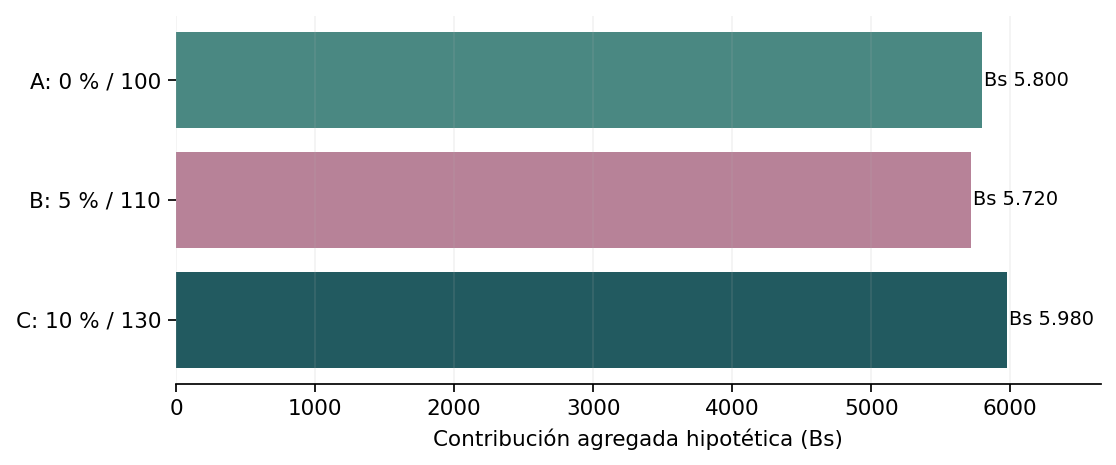
\includegraphics[width=0.9\linewidth]{img/fig_contribucion.png}
\end{figure}
\nota{Los volúmenes de servicios son supuestos, no pronósticos.}

\subsection{Matriz de alternativas, criterios y sensibilidad}

Como primer mecanismo de selección, el equipo desarrollará una matriz de puntuación ponderada exploratoria. Se proponen cuatro criterios con puntuaciones del 1 al 5 (5 representa mejor desempeño), normalizadas antes de sumar. Los pesos son una configuración de ejemplo que requiere validación de la propietaria. Los valores cualitativos de riesgo y facilidad deben justificarse con evidencia o juicio explícito, sin aparecer como resultados objetivos.


\vspace{8pt}{\small\setstretch{1.0}
\begin{longtable}{>{\raggedright\arraybackslash}p{0.2000\dimexpr\linewidth-10\tabcolsep\relax}>{\raggedright\arraybackslash}p{0.2000\dimexpr\linewidth-10\tabcolsep\relax}>{\raggedright\arraybackslash}p{0.2000\dimexpr\linewidth-10\tabcolsep\relax}>{\raggedright\arraybackslash}p{0.2000\dimexpr\linewidth-10\tabcolsep\relax}>{\raggedright\arraybackslash}p{0.2000\dimexpr\linewidth-10\tabcolsep\relax}}
\caption{Matriz ponderada de ejemplo; la puntuación es ilustrativa, dependiente de los criterios y pesos definidos}\label{tab:dss_12}\\
\toprule
\textbf{Criterio} & \textbf{Peso} & \textbf{A} & \textbf{B} & \textbf{C} \\
\midrule\endfirsthead
\toprule
\textbf{Criterio} & \textbf{Peso} & \textbf{A} & \textbf{B} & \textbf{C} \\
\midrule\endhead
\bottomrule\endfoot
\bottomrule\endlastfoot
Contribución mensual esperada & 40~\% & 4 & 3 & 5 \\
Liquidez y previsibilidad & 25~\% & 5 & 4 & 3 \\
Riesgo de demanda & 20~\% & 5 & 4 & 2 \\
Facilidad de operación & 15~\% & 5 & 4 & 3 \\
Puntaje ponderado & 100~\% & 4,60 & 3,60 & 3,60 \\
\end{longtable}}

Con la ponderación del ejemplo, A ocupa el primer lugar por su menor incertidumbre, aunque C genere más contribución bajo el escenario de volumen asumido. Si el peso de la contribución pasa del 40~\% al 75~\% y se reducen proporcionalmente los demás criterios, C podría pasar a ser preferida. Esta sensibilidad deberá calcularse automáticamente y visualizarse, no ocultarse. Cuando existan criterios de exclusión (por ejemplo, incumplimiento de límites aprobados de descuentos), las alternativas no elegibles se descartan antes del ranking.


La matriz de pesos constituye una herramienta didáctica de análisis multicriterio; no debe presentarse como aplicación exhaustiva de MCDA. La evaluación posterior puede incorporar valoración de rangos, compensaciones, incertidumbre y revisión de escalas conforme a guías especializadas.


\subsection{Motor prescriptivo y protocolo de explicación}

Cada recomendación expondrá seis elementos obligatorios: problema de decisión; alternativas y criterios; datos de procedencia; operaciones realizadas; supuestos y límites; y alternativa sugerida con necesidad de aprobación. Si faltan precios vigentes, costos directos o cantidades confiables, el motor mostrará “evidencia insuficiente” y propondrá obtener la información, no inventar una conclusión. La capa generativa solo podrá traducir una estructura de resultados ya calculados por el backend.


\vspace{8pt}{\small\setstretch{1.0}
\begin{longtable}{>{\raggedright\arraybackslash}p{0.3333\dimexpr\linewidth-6\tabcolsep\relax}>{\raggedright\arraybackslash}p{0.3333\dimexpr\linewidth-6\tabcolsep\relax}>{\raggedright\arraybackslash}p{0.3333\dimexpr\linewidth-6\tabcolsep\relax}}
\caption{Trazabilidad de una recomendación desde la información hasta su aprobación}\label{tab:dss_13}\\
\toprule
\textbf{Entrada} & \textbf{Proceso controlado} & \textbf{Salida} \\
\midrule\endfirsthead
\toprule
\textbf{Entrada} & \textbf{Proceso controlado} & \textbf{Salida} \\
\midrule\endhead
\bottomrule\endfoot
\bottomrule\endlastfoot
Movimientos y catálogo & Consulta agregada y autorizada & Indicadores comprobables \\
Escenarios y parámetros & Motor Decimal y simulaciones & Tabla comparativa, umbrales \\
Criterios y pesos & Matriz y sensibilidad & Orden condicional de alternativas \\
Datos, límites y resultados & Plantilla + explicación LLM opcional & Texto con trazas y advertencias \\
Aprobación humana & Bitácora de decisión & Registro y fecha de revisión \\
\end{longtable}}

\subsection{Proyección de caja y análisis de riesgo}

La proyección de caja será distinta a la rentabilidad: partirá de saldos conciliados, cobros efectivamente disponibles, pagos previstos y fechas de vencimiento. La propuesta inicial admite escenarios bajo, base y alto basados en rangos editables. Los pronósticos estadísticos quedan condicionados a contar con un historial temporal suficiente y a evaluar el error de predicción mediante separación temporal de datos (scikit-learn Developers, s. f.-b). El sistema no afirmará capacidad predictiva hasta superar esa validación.


Un tablero de riesgo puede mostrar el efecto de variaciones del volumen de servicios, materiales o descuentos. En esta fase se recomienda análisis de escenarios y sensibilidad determinista antes que simulaciones probabilísticas complejas, porque las distribuciones de probabilidad requerirían justificación adicional.


\subsection{Optimización de capacidad como funcionalidad experimental}

Si el salón registra duración promedio y disponibilidad voluntariamente autorizada por cada especialista, un módulo experimental puede plantear una optimización: maximizar contribución esperada sujeta a horas disponibles y restricciones operativas. Se propone explorar programación lineal mediante SciPy (función linprog) o programación entera cuando se necesiten cantidades discretas. El resultado sería una alternativa de planificación, no una agenda automática ni una instrucción rígida para las trabajadoras.


Modelo orientativo: maximizar $\sum$ $U_i$ × $x_i$ sujeto a $\sum$ $t_i$ × $x_i$ $\leq$ H, $x_i$ $\geq$ 0 y, cuando corresponda, valores enteros. Esta simplificación no captura preferencias de clientas, diferencias de habilidades ni variaciones reales de demanda; por ello solo se incluirá si los datos permiten explicar sus límites.


\subsection{Registro y aprendizaje de las decisiones}

\vspace{8pt}{\small\setstretch{1.0}
\begin{longtable}{>{\raggedright\arraybackslash}p{0.5000\dimexpr\linewidth-4\tabcolsep\relax}>{\raggedright\arraybackslash}p{0.5000\dimexpr\linewidth-4\tabcolsep\relax}}
\caption{Modelo mínimo de auditoría de decisiones (registro propuesto)}\label{tab:dss_14}\\
\toprule
\textbf{Campo} & \textbf{Descripción} \\
\midrule\endfirsthead
\toprule
\textbf{Campo} & \textbf{Descripción} \\
\midrule\endhead
\bottomrule\endfoot
\bottomrule\endlastfoot
decision\_id / salon\_id & Identificación y aislamiento de cada decisión \\
problema / responsable & Cuestión planteada y persona que aprueba \\
alternativas / criterios / pesos & Instantánea de opciones y modelo usado \\
supuestos / fuente de datos & Origen, versión y confiabilidad de la información \\
recomendación / decisión final & Propuesta del sistema y elección efectiva \\
resultado esperado / fecha de revisión & Meta verificable y periodo de seguimiento \\
resultado observado / comentario & Evidencia posterior y explicación de diferencias \\
\end{longtable}}

El historial servirá para mejorar la calidad del proceso, no para automatizar atribuciones causales. Por ejemplo, si después de un descuento aumentan las ventas, el sistema registrará la coincidencia temporal pero no concluirá que el descuento causó el cambio sin evidencia apropiada.


\begin{figure}[H]
\caption{Ciclo propuesto para transformar datos financieros en decisiones humanas revisables}\label{fig:dss_5}
\centering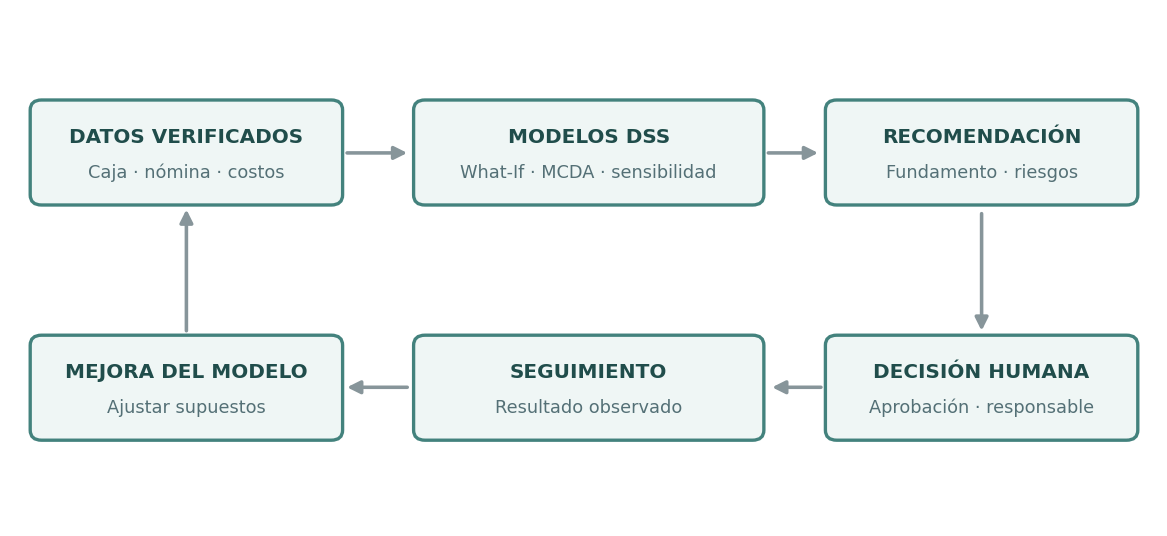
\includegraphics[width=0.9\linewidth]{img/fig_ciclo_decision.png}
\end{figure}
\nota{Elaboración propia.}

\subsection{Requisitos funcionales adicionales del DSS}

\vspace{8pt}{\small\setstretch{1.0}
\begin{longtable}{>{\raggedright\arraybackslash}p{0.3333\dimexpr\linewidth-6\tabcolsep\relax}>{\raggedright\arraybackslash}p{0.3333\dimexpr\linewidth-6\tabcolsep\relax}>{\raggedright\arraybackslash}p{0.3333\dimexpr\linewidth-6\tabcolsep\relax}}
\caption{Requisitos del módulo de soporte para decisiones; deben validarse con el negocio}\label{tab:dss_15}\\
\toprule
\textbf{Código} & \textbf{Requisito verificable} & \textbf{Prioridad} \\
\midrule\endfirsthead
\toprule
\textbf{Código} & \textbf{Requisito verificable} & \textbf{Prioridad} \\
\midrule\endhead
\bottomrule\endfoot
\bottomrule\endlastfoot
DSS-01 & Calcular contribución por servicio con costos directos configurables y trazables & MVP \\
DSS-02 & Crear, editar y comparar al menos tres escenarios sin modificar datos reales & MVP \\
DSS-03 & Aplicar matriz de criterios, pesos normalizados y umbrales de exclusión & MVP \\
DSS-04 & Realizar sensibilidad ante variaciones de pesos y demanda & MVP \\
DSS-05 & Producir recomendación con datos, supuestos, cálculos y advertencias & MVP \\
DSS-06 & Solicitar aprobación humana antes de aplicar una decisión & MVP \\
DSS-07 & Guardar decisiones, resultados esperados y revisión posterior & MVP \\
DSS-08 & Proyectar saldo de caja con escenarios de entradas y salidas & Extensión \\
DSS-09 & Optimizar capacidad usando restricciones de tiempo y disponibilidad & Experimental \\
DSS-10 & Entrenar y validar pronósticos con historial suficiente & Futuro \\
\end{longtable}}

\section{Diseño y Arquitectura de Software}\label{cap:arquitectura}

La arquitectura original del sistema (Figura~\ref{fig:v4_2}) se mantiene como monolito modular y se amplía con los componentes de la propuesta Lush Beauty Smart. Este capítulo detalla sus principios, paquetes, modelo de datos, reglas de negocio, mecanismos de sincronización, seguridad y despliegue.

\subsection{Principios de arquitectura}

La solución adopta un monolito modular con capas de presentación, aplicación, dominio y persistencia. Los módulos se comunican mediante interfaces de servicio declaradas y no acceden directamente a tablas ajenas. La API constituye la autoridad sobre autenticación, validación, cálculos, auditoría y permisos. La IA consulta datos a través de servicios explícitos, y n8n recibe eventos derivados de operaciones confirmadas. La separación permite sustituir proveedores de IA o canales de notificación sin alterar la lógica contable.


\begin{figure}[H]
\caption{Arquitectura conceptual de Lush Beauty Smart}\label{fig:dss_2}
\centering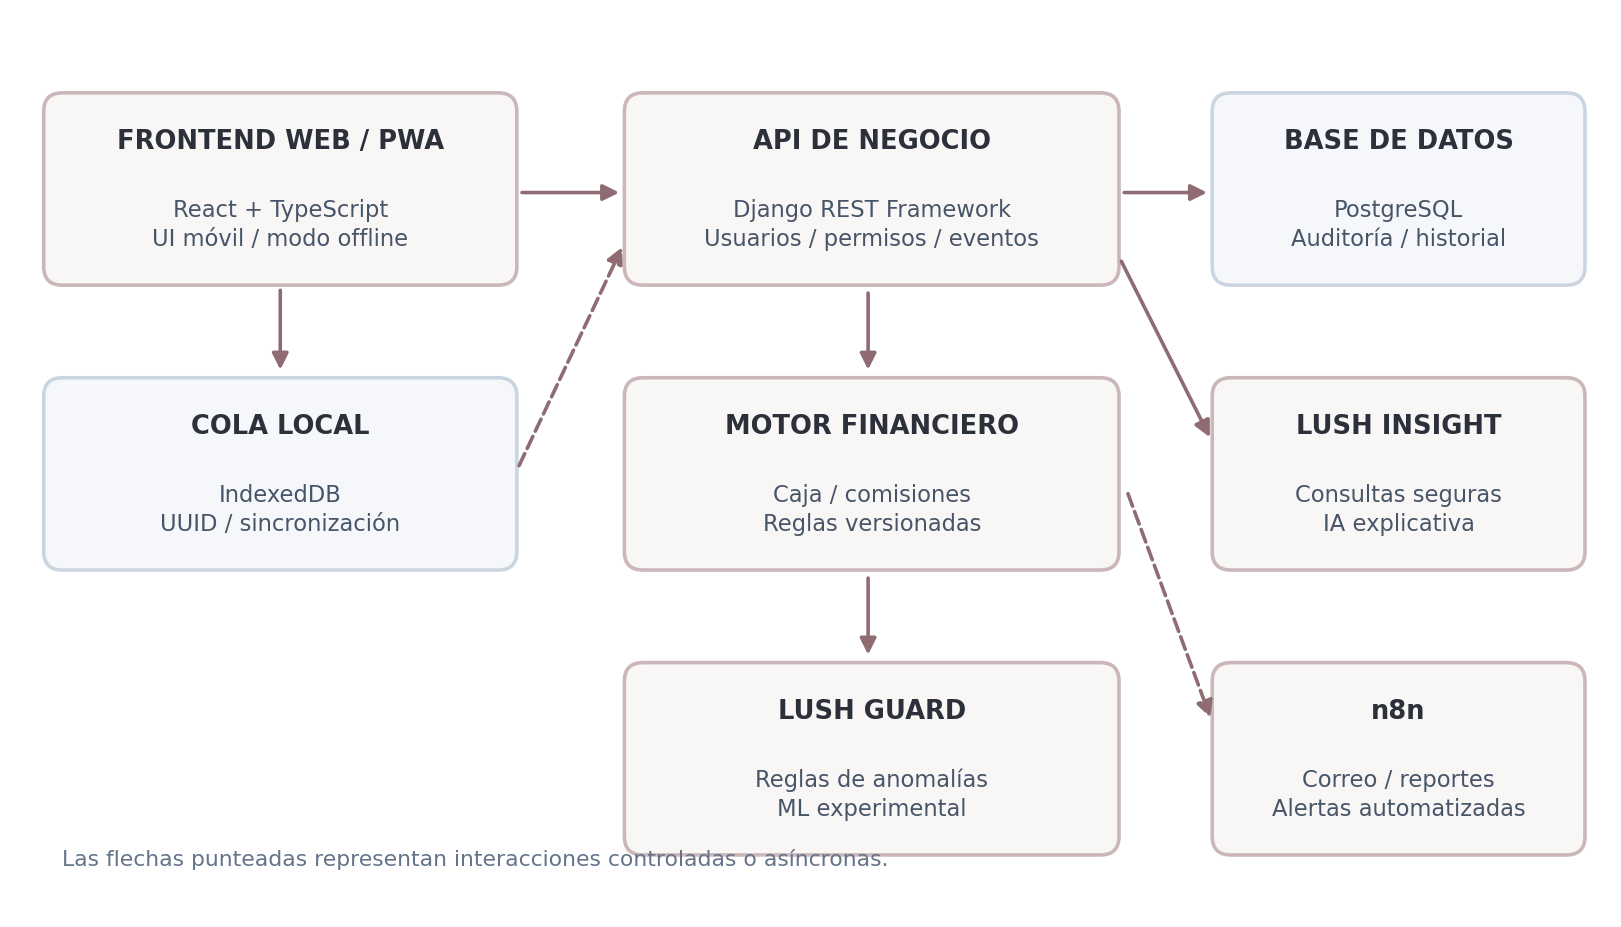
\includegraphics[width=0.9\linewidth]{img/fig_arquitectura_smart.png}
\end{figure}
\nota{Elaboración propia; no representa componentes desplegados en producción.}

\subsubsection{Incorporación de la capa de modelos DSS}

La arquitectura existente se mantiene como monolito modular. Se agregan paquetes independientes: decision\_scenarios para escenarios y sus parámetros, financial\_models para cálculo de contribución y proyección de caja, criteria\_evaluation para matriz y sensibilidad, recommendations para ensamblar explicaciones y decision\_outcomes para seguimiento. El API permite consultas de resultados, pero impide a un LLM invocar escrituras financieras directas. Los servicios DSS consumen datos agregados y snapshots versionados desde PostgreSQL; n8n solo reacciona a decisiones aprobadas.


\vspace{8pt}{\small\setstretch{1.0}
\begin{longtable}{>{\raggedright\arraybackslash}p{0.3333\dimexpr\linewidth-6\tabcolsep\relax}>{\raggedright\arraybackslash}p{0.3333\dimexpr\linewidth-6\tabcolsep\relax}>{\raggedright\arraybackslash}p{0.3333\dimexpr\linewidth-6\tabcolsep\relax}}
\caption{Paquetes adicionales del monolito para implementar el DSS}\label{tab:dss_16}\\
\toprule
\textbf{Servicio backend} & \textbf{Entradas} & \textbf{Salidas / controles} \\
\midrule\endfirsthead
\toprule
\textbf{Servicio backend} & \textbf{Entradas} & \textbf{Salidas / controles} \\
\midrule\endhead
\bottomrule\endfoot
\bottomrule\endlastfoot
financial\_models & Ventas, políticas, costos variables & Decimal; resultados con snapshot \\
decision\_scenarios & Parámetros no operativos de simulación & Resultados comparables y sin escrituras en ventas \\
criteria\_evaluation & Alternativas, escalas, pesos, restricciones & Puntuaciones, ranking y sensibilidad \\
recommendations & Resultados DSS ya calculados & Explicación trazable y estado de evidencia \\
decision\_outcomes & Aprobaciones y revisión posterior & Historial auditable y control por roles \\
\end{longtable}}

\subsection{Componentes y responsabilidades}

\vspace{8pt}{\small\setstretch{1.0}
\begin{longtable}{>{\raggedright\arraybackslash}p{0.3333\dimexpr\linewidth-6\tabcolsep\relax}>{\raggedright\arraybackslash}p{0.3333\dimexpr\linewidth-6\tabcolsep\relax}>{\raggedright\arraybackslash}p{0.3333\dimexpr\linewidth-6\tabcolsep\relax}}
\caption{Selección tecnológica propuesta; versiones concretas deben fijarse al iniciar el repositorio}\label{tab:dss_5}\\
\toprule
\textbf{Componente} & \textbf{Tecnología recomendada} & \textbf{Responsabilidad} \\
\midrule\endfirsthead
\toprule
\textbf{Componente} & \textbf{Tecnología recomendada} & \textbf{Responsabilidad} \\
\midrule\endhead
\bottomrule\endfoot
\bottomrule\endlastfoot
Cliente web/PWA & React, TypeScript & Registro, panel, consultas, estado offline \\
Caché y cola local & Service Worker, IndexedDB & Persistencia temporal y reintentos \\
API REST & Django, DRF & Identidad, permisos, validaciones, consultas \\
Dominio financiero & Python Decimal, servicios Django & Caja, comisiones, nómina, cierres \\
Base de datos & PostgreSQL & Entidades, constraints, snapshots, auditoría \\
Importador & openpyxl, RapidFuzz & Lectura XLSX, normalización y revisión \\
Lush Insight & LLM + herramientas de lectura & Explicaciones ancladas en consultas \\
Lush Guard & Reglas; scikit-learn opcional & Detección y clasificación de incidencias \\
Automatización & n8n, webhooks, eventos & Notificaciones y distribución controlada \\
Despliegue & Docker Compose, HTTPS & Reproducibilidad y entorno de feria \\
\end{longtable}}

\subsection{Modelo conceptual de datos}

Para mantener la trazabilidad se propone modelar cada transacción y cada regla en entidades explícitas. Las relaciones entre servicios, líneas de venta y pagos permitirán representar combos y pagos divididos sin fórmulas incrustadas en el frontend. Una liquidación aprobada conservará su versión y un detalle reproducible de cada concepto.


\vspace{8pt}{\small\setstretch{1.0}
\begin{longtable}{>{\raggedright\arraybackslash}p{0.3333\dimexpr\linewidth-6\tabcolsep\relax}>{\raggedright\arraybackslash}p{0.3333\dimexpr\linewidth-6\tabcolsep\relax}>{\raggedright\arraybackslash}p{0.3333\dimexpr\linewidth-6\tabcolsep\relax}}
\caption{Modelo conceptual inicial; los tipos de datos, índices y cardinalidades se especificarán en el diseño físico}\label{tab:dss_6}\\
\toprule
\textbf{Entidad} & \textbf{Campos fundamentales} & \textbf{Relación principal} \\
\midrule\endfirsthead
\toprule
\textbf{Entidad} & \textbf{Campos fundamentales} & \textbf{Relación principal} \\
\midrule\endhead
\bottomrule\endfoot
\bottomrule\endlastfoot
Salon & id, nombre, estado & Agrupa datos por tenant\_id \\
Usuario / Rol & id, salon\_id, rol, permisos & Acceso por operación \\
Especialista & id, salon\_id, usuario\_id & Realiza servicios \\
ServicioCatalogo & id, nombre, precio, vigencia & Identificado por líneas \\
Venta / LineaVenta & id, uuid\_cliente, importes, snapshots & Servicio y comisión aplicada \\
Pago & id, venta\_id, medio, monto & Distribución por método \\
ReglaComision & id, porcentaje, base, fecha\_inicio & Versión aplicada a líneas \\
Propina / Deduccion & id, especialista, importe, motivo & Integran liquidaciones \\
Liquidacion / Detalle & id, periodo, estado, total & Resumen firmado lógicamente \\
CierreCaja & id, fecha, diferencias, aprobador & Conciliación diaria \\
Auditoria / EventoOutbox & id, actor, antes/después, evento & Trazabilidad y automatización \\
Importacion / Incidencia & id, archivo, fila, estado & Correcciones supervisadas \\
\end{longtable}}

\subsection{Reglas de negocio críticas}

\begin{vinetas}
\item RN-01. Cada venta confirmada dispone de identificador único; los reintentos con la misma clave de idempotencia no crean duplicados.
\item RN-02. Una comisión usa porcentaje, base de cálculo y versión de regla vigentes al momento de la operación.
\item RN-03. Las sumas monetarias emplean Decimal y un criterio explícito de redondeo consistente con el acuerdo del salón.
\item RN-04. La suma de pagos confirmados debe coincidir con el importe cobrable, salvo estados parciales autorizados.
\item RN-05. Una liquidación aprobada no se sobrescribe; cualquier corrección genera un ajuste auditado.
\item RN-06. La especialista solo puede acceder a sus propios detalles y a datos operativos permitidos; la administradora autoriza políticas y cierres.
\item RN-07. Una incidencia detectada por IA o reglas no modifica por sí misma el registro financiero.
\item RN-08. Toda exportación o entrega de información salarial se limita al destinatario autorizado.
\end{vinetas}

\subsection{Sincronización offline e idempotencia}

Al registrar una venta, la PWA guarda una copia estructurada en IndexedDB y asigna un identificador idempotente. El proceso de sincronización transmite registros pendientes cuando hay red. El servidor verifica permisos, integridad, versiones del catálogo y presencia previa de la clave; confirma la transacción en un bloque atómico y devuelve su identificador. Si la red falla después de persistir la operación pero antes de recibir la respuesta, la repetición retorna el resultado original, evitando duplicidad.


Los conflictos se registran para resolución visible: por ejemplo, un precio que cambió mientras la venta estaba fuera de línea o un descuento no autorizado. El cliente no debe convertir un conflicto en una venta confirmada sin intervención. Las pruebas contemplan pérdida de red antes y después de enviar, dos intentos consecutivos y reinicio del teléfono.


\subsection{Diseño de Lush Insight}

El asistente opera con arquitectura de herramientas (tool calling) controladas. Una primera capa verifica el usuario y su tenant; una segunda clasifica la intención y valida fechas; una tercera invoca consultas de solo lectura definidas por contrato, que calculan métricas desde el dominio financiero; finalmente el modelo genera una redacción comprensible a partir de JSON de resultados. Se registran versión del prompt, herramienta consultada, filtros y referencia al reporte, evitando almacenar conversaciones con información sensible sin necesidad.


Ejemplo de contrato: obtener\_impacto\_descuentos(fecha\_inicio, fecha\_fin) devuelve monto\_bruto, descuentos, monto\_neto, comision\_lista, comision\_neto y politica\_vigente. La explicación puede comparar escenarios, pero nunca establecer un cambio de comisión ni ejecutar una transacción. Las respuestas sensibles requieren permisos específicos y se limitan a los períodos autorizados.


\subsection{Arquitectura de eventos y n8n}

Un patrón outbox transaccional permite insertar, junto con la operación aprobada, un evento pendiente de entrega. Un proceso posterior publica al webhook de n8n, que valida el mensaje y ejecuta acciones idempotentes. Si se produce un error temporal en el correo, el flujo puede reintentarse sin volver a contabilizar la nómina. El evento no contendrá más información de la necesaria; para documentos individuales se utilizarán enlaces de expiración corta con control de autorización.


\subsection{Seguridad, privacidad y observabilidad}

El despliegue debe utilizar HTTPS, autenticación robusta, roles, validación de entrada, control de acceso por salón en todas las consultas y registro de eventos críticos. El diseño plantea seguridad a nivel de fila (RLS); su implementación necesita pruebas que demuestren aislamiento efectivo, no solo la presencia de tenant\_id. La copia de seguridad deberá verificarse mediante restauración en un entorno de prueba. Los secretos de n8n y del proveedor de IA no se incluirán en el repositorio.


Los datos enviados a servicios de IA externos, si se utilizan, deben minimizarse y anonimizarse cuando sea posible. Se requiere autorización para procesar información del salón y evitar exponer nombres, teléfonos, salarios y detalles sensibles de clientes en logs o ejemplos de feria. En el entorno demostrativo se recomiendan registros sintéticos y nombres sustituidos por códigos.


\subsection{Estrategia de despliegue y mantenimiento}

Para la feria, Docker Compose puede levantar API, base de datos, frontend y n8n en un entorno reproducible. Se separan ambientes de desarrollo, demostración y piloto; no se reutiliza la base real en una demostración pública. Se documentan variables de entorno, copias de seguridad, migraciones, cuentas de prueba y un plan de funcionamiento sin servicio de IA: la caja, las comisiones y los reportes deben seguir operando cuando no esté disponible el asistente.


\section{Hipótesis}\label{cap:hipotesis}

La hipótesis expresa una respuesta tentativa al problema formulado, que será contrastada con los datos de la línea base retrospectiva del salón y de las semanas de prueba piloto.


\textbf{Hipótesis de investigación (Hi):} Si se implementa el sistema web móvil Lush Beauty para la gestión de caja y nómina, entonces disminuyen el tiempo de liquidación semanal y la tasa de errores de cálculo de comisiones en el salón Lush Beauty de la ciudad de Santa Cruz de la Sierra durante el piloto de enero de 2027.


\textbf{Hipótesis nula ($H_0$):} La implementación del sistema web móvil Lush Beauty no tiene un efecto significativo en el tiempo de liquidación semanal ni en la tasa de errores de cálculo de comisiones del salón.


\textbf{Hipótesis alternativa (Ha):} La implementación del sistema web móvil Lush Beauty tiene un efecto significativo en el tiempo de liquidación semanal y/o en la tasa de errores de cálculo de comisiones.


\subsection{Hipótesis para el soporte a decisiones}

La ampliación hacia el soporte para decisiones incorpora, además, las siguientes hipótesis de trabajo, referidas a tareas estructuradas de comparación financiera en el entorno piloto.

Hipótesis de investigación (Hi): El uso del prototipo Lush Beauty Smart DSS permitirá a las participantes completar tareas estructuradas de comparación financiera con menos tiempo y mayor trazabilidad de criterios que con el procedimiento manual basado en hojas de cálculo, en el entorno piloto definido para el estudio.


Hipótesis nula ($H_0$): En las tareas estructuradas del piloto, no se observará una mejora en el tiempo de comparación de alternativas ni en la trazabilidad de criterios respecto del procedimiento manual.


Hipótesis alternativa operativa (Ha): Se observará mejora en al menos uno de los indicadores de tiempo o trazabilidad; cualquier diferencia deberá interpretarse con prudencia por el tamaño reducido de la muestra y la ausencia de grupo de control.


\section{Operacionalización de la Hipótesis}\label{cap:operacionalizacion}

La Tabla~\ref{tab:v4_4} traduce las variables en dimensiones, indicadores e instrumentos medibles. La variable independiente corresponde a la implementación del sistema; la dependiente, a la eficiencia y exactitud de la gestión administrativa.


\vspace{8pt}{\footnotesize\setstretch{1.0}
\begin{longtable}{>{\raggedright\arraybackslash}p{0.1434\dimexpr\linewidth-12\tabcolsep\relax}>{\raggedright\arraybackslash}p{0.1992\dimexpr\linewidth-12\tabcolsep\relax}>{\raggedright\arraybackslash}p{0.1713\dimexpr\linewidth-12\tabcolsep\relax}>{\raggedright\arraybackslash}p{0.1355\dimexpr\linewidth-12\tabcolsep\relax}>{\raggedright\arraybackslash}p{0.1952\dimexpr\linewidth-12\tabcolsep\relax}>{\raggedright\arraybackslash}p{0.1554\dimexpr\linewidth-12\tabcolsep\relax}}
\caption{Operacionalización de las variables}\label{tab:v4_4}\\
\toprule
\textbf{Variable} & \textbf{Definición conceptual} & \textbf{Definición operacional} & \textbf{Dimensión} & \textbf{Indicadores} & \textbf{Escala / instrumento} \\
\midrule\endfirsthead
\toprule
\textbf{Variable} & \textbf{Definición conceptual} & \textbf{Definición operacional} & \textbf{Dimensión} & \textbf{Indicadores} & \textbf{Escala / instrumento} \\
\midrule\endhead
\bottomrule\endfoot
\bottomrule\endlastfoot
\textbf{Independiente (causa):} implementación del sistema web móvil Lush Beauty & Sistema de información que recopila, procesa y distribuye datos para apoyar el control de la organización (Laudon \& Laudon, 2016), cuya calidad en uso se evalúa según ISO/IEC (2011). & Sistema operando en el salón, con registro de servicios contra catálogo, caja diaria y liquidación automática. & 1. Cobertura funcional\newline{}2. Usabilidad percibida & \% de servicios registrados vinculados al catálogo; n.º de funciones operativas del MVP; puntaje SUS (0–100). & Razón / ficha de verificación funcional; ordinal-intervalo / cuestionario SUS (Brooke, 1996). \\
\textbf{Dependiente (efecto):} eficiencia y exactitud de la gestión administrativa & Grado en que los procesos de registro y liquidación se completan con el menor consumo de tiempo y sin desviaciones respecto del resultado correcto (ISO/IEC, 2011; DeLone \& McLean, 2003). & Diferencia entre la línea base retrospectiva y las semanas piloto en tiempo y en discrepancias de cálculo. & 1. Eficiencia temporal\newline{}2. Exactitud del cálculo\newline{}3. Trazabilidad & Minutos por liquidación semanal; segundos por registro de servicio;~\% de líneas con discrepancia de comisión;~\% de liquidaciones con diferencia;~\% de registros con método de pago y bitácora. & Razón / ficha de observación cronometrada y ficha de conciliación contra cálculo de referencia. \\
\end{longtable}}
\nota{Elaboración propia. SUS: System Usability Scale.}

\subsection{Variables e indicadores del soporte para decisiones}

\vspace{8pt}{\small\setstretch{1.0}
\begin{longtable}{>{\raggedright\arraybackslash}p{0.2500\dimexpr\linewidth-8\tabcolsep\relax}>{\raggedright\arraybackslash}p{0.2500\dimexpr\linewidth-8\tabcolsep\relax}>{\raggedright\arraybackslash}p{0.2500\dimexpr\linewidth-8\tabcolsep\relax}>{\raggedright\arraybackslash}p{0.2500\dimexpr\linewidth-8\tabcolsep\relax}}
\caption{Operacionalización ampliada del soporte para decisiones}\label{tab:dss_17}\\
\toprule
\textbf{Variable} & \textbf{Dimensión} & \textbf{Indicador} & \textbf{Medición} \\
\midrule\endfirsthead
\toprule
\textbf{Variable} & \textbf{Dimensión} & \textbf{Indicador} & \textbf{Medición} \\
\midrule\endhead
\bottomrule\endfoot
\bottomrule\endlastfoot
Independiente: uso DSS & Cobertura del proceso & \% de decisiones con alternativas y criterios completos & Lista de verificación \\
Dependiente: calidad del proceso & Eficiencia & Minutos por tarea de comparación & Observación cronometrada \\
Dependiente: calidad del proceso & Trazabilidad & \% decisiones con fuentes, supuestos y aprobación & Auditoría \\
Dependiente: calidad del proceso & Comprensión & Explicación correcta de las razones de la recomendación & Guía breve de evaluación \\
Técnica: motor de escenarios & Exactitud & \% de cálculos coincidentes con referencia independiente & Casos unitarios \\
Técnica: recomendaciones & Seguridad & N.º de acciones financieras efectuadas sin aprobación & Pruebas de permisos \\
Seguimiento & Contraste & Diferencia entre indicador esperado y observado & Registro de decisiones \\
\end{longtable}}
\nota{Elaboración propia. Indicadores de evaluación propuestos, no medidos.}

\subsection{Precauciones de interpretación}

No se inferirá causalidad fuerte sobre mejoras económicas a partir de un solo salón y pocas participantes. Se priorizarán validaciones deterministas del motor matemático y pruebas de tareas repetibles con tiempo y observación. Las encuestas de usabilidad y percepción se presentarán como evidencia descriptiva. Para estudiar impacto comercial real de una promoción se requeriría diseño adicional, autorización y observaciones suficientes.


\section{Marco Metodológico}\label{cap:metodologico}

\subsection{Tipo y diseño de investigación}

\vspace{8pt}{\small\setstretch{1.0}
\begin{longtable}{>{\raggedright\arraybackslash}p{0.1829\dimexpr\linewidth-6\tabcolsep\relax}>{\raggedright\arraybackslash}p{0.3902\dimexpr\linewidth-6\tabcolsep\relax}>{\raggedright\arraybackslash}p{0.4269\dimexpr\linewidth-6\tabcolsep\relax}}
\caption{Características metodológicas de la investigación}\label{tab:v4_5}\\
\toprule
\textbf{Criterio} & \textbf{Elección} & \textbf{Justificación} \\
\midrule\endfirsthead
\toprule
\textbf{Criterio} & \textbf{Elección} & \textbf{Justificación} \\
\midrule\endhead
\bottomrule\endfoot
\bottomrule\endlastfoot
Enfoque & Cuantitativo con apoyo cualitativo (mixto con predominio cuantitativo) & Se miden tiempos y errores; la entrevista complementa la interpretación \\
Alcance & Descriptivo y explicativo & Describe el proceso actual y explica el efecto del sistema sobre las variables \\
Diseño & Preexperimental de preprueba y posprueba con un solo grupo & Existe un único salón; la línea base retrospectiva (registros previos del salón) actúa como preprueba \\
Temporalidad & Longitudinal corto (cuatro semanas de línea base retrospectiva y cuatro de piloto) & Permite comparar semanas equivalentes \\
Fuentes & Primarias (campo) con apoyo documental & Registros del salón, cuestionario de requerimientos, observación cronometrada y catálogo oficial \\
\end{longtable}}
\nota{Elaboración propia con base en Hernández Sampieri et al. (2014).}

El enfoque y el diseño se establecieron conforme a las categorías propuestas por Hernández Sampieri et al. (2014). Se reconoce como limitación del diseño la ausencia de grupo de control, por lo que los resultados se interpretarán con cautela y se complementarán con la bitácora del sistema y con la entrevista a la administradora.


La propuesta conserva la orientación aplicada, con mediciones cuantitativas complementadas por entrevistas y observación. El estudio establece un diseño preexperimental de preprueba y posprueba con un único salón, cuatro semanas retrospectivas y cuatro semanas de piloto. La incorporación de nuevas funciones exige añadir instrumentos de control, pero no modificar los objetivos de forma que se atribuyan resultados a IA sin un contraste específico. No se plantea un grupo de control inexistente.


\subsection{Población y muestra}

\textbf{Población.} Está conformada por (a) las tres personas que prestan servicios en el salón, incluida la administradora, y (b) los registros de servicios de las cuatro semanas previas al piloto, que constituyen la línea base retrospectiva, más los registros generados durante el piloto. La planilla de ejemplo de agosto de 2026, con 91 registros en un mes, se usa solo como referencia de volumen.


\textbf{Muestra.} No se realiza muestreo. Dado el tamaño reducido de la población, se trabajará con un \textbf{censo}, es decir, con la totalidad de las tres trabajadoras y de los registros del periodo de estudio. Como referencia, una muestra de registros calculada con la fórmula para poblaciones finitas, n = N·Z²·p·q / [e²(N−1) + Z²·p·q], con N = 91, Z = 1,96, p = q = 0,5 y e = 0,05, requeriría 74 registros; por ello se verificará la totalidad de los registros.


\textbf{Criterios de inclusión:} personal activo del salón durante el periodo de estudio; registros de servicios con estado completado; participación voluntaria. \textbf{Criterios de exclusión:} servicios cancelados (no generan comisión), registros duplicados y personal que no utilice el sistema durante el piloto.


La población del piloto comprende a las tres personas del salón y los registros del período evaluado. Dado el número reducido de trabajadoras, se considera un censo para las encuestas, complementado con la revisión completa de transacciones disponibles. La planilla de 91 registros se usa únicamente para comprobar reglas y construir casos reproducibles; no debe interpretarse como un conjunto suficiente para entrenar un modelo generalizable.


\subsection{Técnicas e instrumentos}

\begin{vinetas}
\item \textbf{Análisis documental:} revisión de la planilla de ejemplo de agosto de 2026, de los registros previos del salón y del catálogo oficial de servicios; instrumento: ficha de análisis documental.
\item \textbf{Cuestionario de requerimientos:} obtención estructurada de las necesidades del salón por módulo, con escala de priorización de uno a cinco; aplicado a la administradora y a las especialistas; instrumento: Anexo A.
\item \textbf{Observación estructurada:} medición cronometrada del registro de servicios, del cierre de caja y de la liquidación; instrumentos: ficha de observación cronometrada y ficha de conciliación (Anexo C).
\item \textbf{Conciliación de cálculos:} comparación de la comisión calculada por el sistema con un cálculo de referencia independiente, primero con la planilla de ejemplo y luego con los registros reales del salón.
\item \textbf{Encuesta de usabilidad:} cuestionario SUS de diez ítems traducido al español (Brooke, 1996); instrumento: Anexo B.
\item \textbf{Entrevista semiestructurada} a la administradora sobre el proceso actual, las dificultades y la adopción del sistema; instrumento: guía de entrevista (Anexo D).
\end{vinetas}

\textbf{Validez y confiabilidad.} Los cuestionarios, las fichas y la guía de entrevista serán validados mediante juicio de expertos, integrado por el docente de la asignatura y un profesional del área de sistemas. Antes de su aplicación se realizará una prueba piloto con una persona del salón que no participe en la muestra, para detectar preguntas ambiguas. El cuestionario SUS es un instrumento estandarizado; su consistencia interna se reportará mediante el alfa de Cronbach (Cronbach, 1951), advirtiendo que con tres respondientes el coeficiente solo tiene valor referencial.


\subsubsection{Instrumentos y procedimiento ampliados}

Se utilizarán el cuestionario de requerimientos, la guía de entrevista, la ficha de observación cronometrada y el cuestionario SUS (Anexos A a D), ajustados para incluir importación, alertas, consultas explicativas y sincronización. La validación técnica tendrá casos de prueba automatizados con resultados de referencia calculados por separado de la implementación. El piloto recogerá condiciones de conectividad, tareas realizadas, tiempos, errores y comentarios de cada usuaria.


La evaluación se organizará en cuatro momentos: establecimiento de la línea base; verificación del motor financiero mediante operaciones conocidas y casos límite; prueba de usabilidad con usuarias y escenarios de atención cotidiana; y análisis descriptivo del piloto. Las diferencias observadas pueden coincidir con cambios de temporada, aprendizaje o carga de trabajo; por lo tanto, no se interpretarán como causalidad demostrada por sí solas.


\subsubsection{Evaluación experimental de decisiones}

Se diseñarán tres tareas equivalentes en papel/Excel y en el DSS: comparar políticas de descuento, evaluar cambio de precio con costos directos y justificar un cierre de caja con diferencia. Para cada una se conservarán los mismos datos de entrada y un cálculo de referencia independiente. Se medirá tiempo de tarea, número de consultas o correcciones, resultado final y capacidad de explicar la decisión. En sesiones con pocas participantes se priorizará comparación descriptiva pareada, evitando exagerar inferencias estadísticas.


Se ejecutarán pruebas metamórficas: al aumentar el descuento manteniendo constantes precio de lista, comisión sobre lista, materiales y cantidad, la contribución unitaria no puede aumentar; al duplicar el volumen con contribución positiva constante, el total debe duplicarse; al redistribuir pesos de criterios, el ranking debe actualizarse de forma reproducible. También se comprobará que los escenarios no cambien ventas reales.


\subsubsection{Evaluación específica de IA y automatización}

La importación inteligente se medirá con un conjunto etiquetado de variantes reales y sintéticas: porcentaje de sugerencias correctas, casos enviados a revisión y errores de aceptación. Lush Insight se evaluará mediante preguntas cerradas con respuesta de referencia, exactitud de cifras, respeto de permisos y manejo de períodos sin información. Lush Guard se comprobará con incidencias inyectadas y casos normales para revisar falsas alarmas. n8n se probará mediante eventos repetidos, error de correo y recuperación controlada. Para el DSS se añadirá un banco de casos con respuestas de referencia: exactitud decimal de contribución, umbral de volumen, puntuación ponderada, sensibilidad de pesos, detección de información insuficiente y cumplimiento de aprobación humana. Las explicaciones generadas se revisarán con una rúbrica de exactitud, trazabilidad, cautela y lenguaje comprensible.


\subsubsection{Indicadores y metas de prueba}

\vspace{8pt}{\small\setstretch{1.0}
\begin{longtable}{>{\raggedright\arraybackslash}p{0.2500\dimexpr\linewidth-8\tabcolsep\relax}>{\raggedright\arraybackslash}p{0.2500\dimexpr\linewidth-8\tabcolsep\relax}>{\raggedright\arraybackslash}p{0.2500\dimexpr\linewidth-8\tabcolsep\relax}>{\raggedright\arraybackslash}p{0.2500\dimexpr\linewidth-8\tabcolsep\relax}}
\caption{Objetivos de prueba y criterios de seguimiento}\label{tab:dss_7}\\
\toprule
\textbf{Dimensión} & \textbf{Indicador} & \textbf{Instrumento} & \textbf{Meta propuesta} \\
\midrule\endfirsthead
\toprule
\textbf{Dimensión} & \textbf{Indicador} & \textbf{Instrumento} & \textbf{Meta propuesta} \\
\midrule\endhead
\bottomrule\endfoot
\bottomrule\endlastfoot
Eficiencia & Tiempo de registro por servicio & Cronometría & < 15 s en flujo habitual \\
Exactitud & Discrepancias de comisión & Conciliación independiente & 0 en casos de prueba \\
Persistencia & Duplicados de ventas offline & Pruebas de reintento & 0 en escenarios probados \\
Trazabilidad & Cambios críticos auditados & Consulta de bitácora & 100~\% de casos cubiertos \\
Calidad de importación & Filas aceptadas o en revisión & Reporte de importación & 100~\% con estado explícito \\
IA explicable & Respuestas fundamentadas & Batería de preguntas & Sin cifras inventadas en pruebas \\
Automatización & Flujos ejecutados y recuperados & Logs de n8n & 3 flujos demostrados \\
Usabilidad & Puntaje SUS y observaciones & Cuestionario / entrevista & Registrar, no prometer valor \\
\end{longtable}}
\nota{Elaboración propia. No representan resultados observados.}

\subsection{Metodología de desarrollo del producto}

El sistema se desarrollará con un marco ágil de trabajo en iteraciones cortas de una a dos semanas (Schwaber \& Sutherland, 2020), priorizando las funciones de caja y nómina del producto mínimo viable. La arquitectura es un monolito modular con interfaz web (React y TypeScript), API REST (Django y Django REST Framework) y base de datos PostgreSQL, conforme a la Figura~\ref{fig:v4_2}. Los cálculos monetarios se realizan en el servidor con tipos decimales para evitar errores de redondeo, y toda modificación queda registrada en una bitácora inmutable.


El detalle de la arquitectura ampliada, de las reglas de negocio y de la estrategia de despliegue se presenta en el Capítulo~\ref{cap:arquitectura}.

\subsection{Procedimiento de análisis}

Los datos se procesarán en hojas de cálculo y en el lenguaje Python, con estadística descriptiva (media, mediana, desviación estándar y porcentajes). Para contrastar la hipótesis, las mediciones de tiempo y de errores se organizan como datos pareados por trabajadora y semana: con tres trabajadoras y cuatro semanas se obtienen n = 12 pares, lo que permite aplicar la prueba de rangos con signo de Wilcoxon sobre los tiempos. Para las proporciones de error, de conteo pequeño, se utilizará la prueba exacta de Fisher. El nivel de significación será α = 0,05. Por el tamaño de la muestra, se reportarán también los tamaños del efecto y los resultados se interpretarán como evidencia de tendencia, no como generalizable.


La entrevista y las respuestas abiertas del cuestionario de requerimientos se analizarán mediante categorías temáticas: proceso actual, dificultades, necesidades priorizadas y adopción.


\textbf{Aspectos éticos.} Se solicitará consentimiento informado a todas las participantes (Anexo E). Se garantizará la confidencialidad de los datos de sueldos y de clientes: los nombres de clientes se sustituirán por códigos y las cifras del salón se presentarán de forma agregada. El acceso al sistema estará restringido por roles, y las cifras se emplearán exclusivamente con fines académicos y con autorización de la propietaria.


\subsection{Limitaciones del estudio}

El diseño tiene limitaciones que se reconocen desde el inicio. Primero, es preexperimental y no cuenta con grupo de control, por lo que las diferencias entre la línea base y el piloto no pueden atribuirse con certeza al sistema: pueden influir factores como la temporada de mayor demanda, los cambios de personal o el efecto de novedad. Segundo, la muestra es de tres trabajadoras, lo que limita la generalización y la potencia de las pruebas estadísticas. Tercero, la administradora participa como propietaria, usuaria y evaluadora del sistema, lo que puede generar sesgo de deseabilidad; para mitigarlo, las encuestas y las entrevistas de las especialistas se aplicarán de forma anónima y se contrastarán con la bitácora del sistema. Cuarto, la planilla de agosto de 2026 es un ejemplo representativo y no un registro operativo, por lo que el diagnóstico se complementa con los registros reales del salón. Finalmente, los precios de los sistemas comerciales son referenciales y pueden cambiar, y no se localizaron antecedentes bolivianos verificables que permitan una comparación local directa.


Se solicitará consentimiento informado al personal, se ocultarán identidades de clientas y se restringirá el acceso a remuneraciones. El Anexo G contiene respuestas ilustrativas derivadas del proyecto, no entrevistas reales; no se usarán como evidencia empírica. Asimismo, la muestra pequeña, el diseño preexperimental y la ausencia de una base histórica extensa limitan la generalización de resultados y la pertinencia de predicción automatizada de ingresos.


\section{Implementación y Resultados Técnicos}\label{cap:implementacion}

Este capítulo documenta lo que existe construido y verificado al 26 de noviembre de 2026 (semana 4 del cronograma). Todas las cifras proceden de ejecuciones realizadas sobre el repositorio en esa fecha o del conteo de su código y esquema; no provienen de datos reales del salón. Los resultados de efecto sobre el tiempo de liquidación, los errores de cálculo y la usabilidad (Capítulo~\ref{cap:operacionalizacion}) \textbf{no se reportan aquí}, porque requieren la medición posterior descrita en el marco metodológico.

\subsection{Alcance construido}

El sistema se implementó como un monolito modular: cada dominio tiene su propia carpeta con reglas puras (\textit{domain}), casos de uso (\textit{services}), adaptador HTTP (\textit{api}), persistencia y un contrato público, de modo que un módulo pueda extraerse como microservicio sin reescribirlo. La Tabla~\ref{tab:impl_1} resume los módulos de backend en operación.

\vspace{8pt}{\small\setstretch{1.0}
\begin{longtable}{>{\raggedright\arraybackslash}p{0.17\linewidth}>{\raggedright\arraybackslash}p{0.60\linewidth}>{\centering\arraybackslash}p{0.15\linewidth}}
\caption{Módulos de backend implementados}\label{tab:impl_1}\\
\toprule
\textbf{Módulo} & \textbf{Responsabilidad} & \textbf{Métodos de prueba} \\
\midrule\endfirsthead
\toprule
\textbf{Módulo} & \textbf{Responsabilidad} & \textbf{Métodos de prueba} \\
\midrule\endhead
\bottomrule\endfoot
\bottomrule\endlastfoot
identity & Salones, usuarios, roles, permisos y autenticación & 28 \\
audit & Historial de cambios con contexto de usuario & 4 \\
catalog & Servicios, especialistas y clientas & 9 \\
commissions & Reglas de comisión versionadas y snapshot por línea de venta & 34 \\
sales & Ventas multilínea, pagos divididos, anulación e idempotencia por UUID & 53 \\
cashier & Resumen y cierre de caja por método de pago & 30 \\
payroll & Deducciones, liquidación semanal, aprobación, pago, PDF y XLSX & 79 \\
analytics & Panel financiero (lectura) & 19 \\
notifications & Bandeja de salida (\textit{outbox}) para n8n & 28 \\
demo & Datos sintéticos para la demostración & 7 \\
\end{longtable}}
\nota{Elaboración propia a partir de \texttt{Backend/lushbeauty/apps/}. Se contaron los métodos \texttt{test\_*} de cada módulo (291); el ejecutor de pruebas reporta 295 casos porque algunos métodos generan más de un caso.}

En el frente de usuario existen dos clientes: la aplicación web progresiva (PWA) de React y TypeScript, organizada por módulos (\textit{sales}, \textit{payroll}, \textit{cashier}, \textit{analytics}, \textit{decisions}, \textit{insight}, \textit{guard}, \textit{imports}, entre otros), y una réplica móvil en Flutter con las vistas de la especialista (ingreso, \textit{Hoy}, registro rápido, sincronización, \textit{Mi liquidación} y cierre de caja). La base de datos PostgreSQL se define en un esquema propio con 23 tablas y 20 políticas de seguridad a nivel de fila (RLS).

\subsection{Verificación ejecutada}

La Tabla~\ref{tab:impl_2} presenta las suites ejecutadas el 26 de noviembre de 2026. El backend se probó contra PostgreSQL dentro de Docker; las pruebas de dominio (comisión, contribución, liquidación) usan \texttt{Decimal} y no requieren base de datos.

\vspace{8pt}{\small\setstretch{1.0}
\begin{longtable}{>{\raggedright\arraybackslash}p{0.28\linewidth}>{\raggedright\arraybackslash}p{0.28\linewidth}>{\centering\arraybackslash}p{0.14\linewidth}>{\raggedright\arraybackslash}p{0.20\linewidth}}
\caption{Pruebas automatizadas ejecutadas}\label{tab:impl_2}\\
\toprule
\textbf{Componente} & \textbf{Herramienta} & \textbf{Casos} & \textbf{Resultado} \\
\midrule\endfirsthead
\toprule
\textbf{Componente} & \textbf{Herramienta} & \textbf{Casos} & \textbf{Resultado} \\
\midrule\endhead
\bottomrule\endfoot
\bottomrule\endlastfoot
Backend Django/DRF & \texttt{manage.py test}, PostgreSQL 17 & 295 & Todos aprobados \\
Web (PWA) & Vitest & 120 & Todos aprobados \\
Móvil (Flutter) & \texttt{flutter test} & 32 & Todos aprobados \\
\end{longtable}}
\nota{Elaboración propia. El número de casos de cada suite es el informado por su ejecutor. No se midió cobertura de código; por tanto, estas cifras indican qué comportamientos están cubiertos, no qué porcentaje del código lo está.}

Entre los comportamientos comprobados por las pruebas se encuentran los siguientes casos de aceptación del Anexo~J:

\begin{vinetas}
\item \textbf{CP-01, descuento sin alterar la lista.} Un servicio de lista Bs~120 con descuento de Bs~8 se cobra a Bs~112; se conserva el precio de lista y la comisión (35\,\% ilustrativo) se calcula sobre la lista: Bs~42,00. Se verifica en dominio, API y pantalla.
\item \textbf{Idempotencia.} Reenviar una venta con el mismo UUID devuelve la existente (201 la primera vez, 200 después) sin crear filas; el mismo UUID en otro salón es otra venta.
\item \textbf{Integridad monetaria.} Pagos distintos de las líneas se rechazan sin dejar filas; el umbral de descuento de 10\,\% pasa sin aprobación y un centavo más la exige.
\item \textbf{Inmutabilidad.} La base de datos no permite borrar ni modificar líneas confirmadas ni liquidaciones aprobadas; la anulación conserva las líneas y queda auditada.
\item \textbf{Aislamiento por salón y por rol.} Un salón no ve datos de otro; una especialista solo ve sus servicios y únicamente sus liquidaciones aprobadas, con su comprobante PDF.
\end{vinetas}

\subsection{Ciclo operativo demostrable}

El ciclo central de caja y nómina funciona de extremo a extremo en el backend: registro de venta con pagos $\rightarrow$ cálculo de comisión por \textit{snapshot} versionado $\rightarrow$ cierre de caja por método $\rightarrow$ borrador y aprobación de la liquidación semanal (sueldo fijo, comisión, propina y deducciones con motivo) $\rightarrow$ marcado como pagada y emisión de comprobante PDF y resumen XLSX. La fórmula de liquidación se aplica igual en el dominio y en una restricción de la base de datos. Los eventos de cierre y de liquidación se escriben en la bandeja de salida para su entrega por n8n.

\subsection{Estado por funcionalidad}

La Tabla~\ref{tab:impl_3} distingue lo implementado de lo que sigue como maqueta. Se toma del backlog del repositorio (\texttt{odd/tasks/INDEX.md}) y se contrastó con el código y las pruebas.

\vspace{8pt}{\small\setstretch{1.0}
\begin{longtable}{>{\raggedright\arraybackslash}p{0.30\linewidth}>{\raggedright\arraybackslash}p{0.34\linewidth}>{\raggedright\arraybackslash}p{0.28\linewidth}}
\caption{Estado de las funcionalidades al 26 de noviembre de 2026}\label{tab:impl_3}\\
\toprule
\textbf{Funcionalidad} & \textbf{Backend} & \textbf{Interfaz} \\
\midrule\endfirsthead
\toprule
\textbf{Funcionalidad} & \textbf{Backend} & \textbf{Interfaz} \\
\midrule\endhead
\bottomrule\endfoot
\bottomrule\endlastfoot
Base y seguridad (F00, F14) & Hecho; RLS, auditoría y datos demo; parcial en despliegue y CI & Solo el inicio de sesión consume la API \\
Caja, ventas y pagos (F01) & Hecho & Maqueta sin conectar \\
Comisiones versionadas (F02) & Hecho & Lectura con datos de prueba \\
Liquidación semanal (F03) & Hecho, con PDF y XLSX & Maqueta \\
Cierre de caja (F04) & Hecho & Maqueta \\
PWA sin conexión (F05) & Idempotencia lista; cola y sincronizador pendientes & Maqueta \\
Importador de Excel (F06) & Sin empezar & Maqueta \\
Panel financiero (F07) & Lectura hecha & Maqueta \\
Contribución y What-If (F08) & Parcial & Maqueta \\
Matriz y sensibilidad (F09) & Sin empezar & Maqueta \\
Recomendación y decisiones (F10) & Sin empezar & Maqueta \\
Lush Insight (F11) y Guard (F12) & Sin empezar & Maqueta / respuestas fijas \\
n8n y \textit{outbox} (F13) & Eventos de cierre y liquidación; faltan los flujos & Sin empezar \\
\end{longtable}}
\nota{Elaboración propia. «Maqueta» significa pantalla con datos en memoria que no llama al API correspondiente, aunque el endpoint exista.}

\subsection{Decisiones abiertas con valor provisional}

Algunas reglas se aplicaron con un valor inicial a la espera de validación con la administradora: el redondeo de la comisión (mitad hacia arriba, a dos decimales), el umbral de descuento sin aprobación (10\,\%), los métodos de pago (efectivo, QR, transferencia y tarjeta), la semana de liquidación (lunes a domingo, configurable por salón) y los pesos por defecto de la matriz de decisión (40/25/20/15, de ejemplo). Los resultados que dependen de ellos deben leerse como condicionados a esa validación.

\subsection{Limitaciones del avance}

\begin{vinetas}
\item La interfaz web aún no consume la mayoría de los endpoints existentes; la integración convertirá las maquetas en pantallas reales.
\item El módulo de soporte para decisiones (escenarios, matriz, sensibilidad, recomendación y seguimiento) carece de backend, salvo un avance parcial del modelo de contribución.
\item No se han hecho pruebas de carga, de concurrencia real ni de campo con conexión intermitente.
\item Las capturas de pantalla de las vistas de la PWA y de Flutter se incorporarán cuando estén conectadas al API; hasta entonces no se presentan como evidencia de funcionamiento.
\item No hay mediciones de tiempo de liquidación, tasa de errores ni usabilidad (SUS); las hipótesis siguen sin contrastarse.
\end{vinetas}

\section{Cronograma de Actividades, Demostración y Riesgos}\label{cap:cronograma}

\subsection{Cronograma general — Diagrama de Gantt}

El cronograma abarca dieciocho semanas, desde el lunes 2 de noviembre de 2026 hasta el domingo 7 de marzo de 2027. Al 16 de noviembre de 2026 el proyecto se encuentra en la semana 3, marcada con un asterisco. Las semanas 16 y 17 se reservan como margen para imprevistos, equivalentes al 11~\% del tiempo total, dentro del rango recomendado del 10~\% al 15~\%. El cronograma se amplió de catorce a dieciocho semanas porque la validación de instrumentos y la línea base retrospectiva no estaban contempladas en la versión anterior.


\begin{landscape}
\captionsetup{width=\linewidth}
{\footnotesize\setstretch{1.0}\setlength{\tabcolsep}{2pt}
\begin{longtable}{p{8.3cm}*{18}{>{\centering\arraybackslash}p{0.55cm}}}
\caption{Cronograma de actividades (18 semanas)}\label{tab:v4_6}\\
\toprule
\textbf{Actividad} & \textbf{S1}\newline{\tiny 02/11} & \textbf{S2}\newline{\tiny 09/11} & \textbf{S3*}\newline{\tiny 16/11} & \textbf{S4}\newline{\tiny 23/11} & \textbf{S5}\newline{\tiny 30/11} & \textbf{S6}\newline{\tiny 07/12} & \textbf{S7}\newline{\tiny 14/12} & \textbf{S8}\newline{\tiny 21/12} & \textbf{S9}\newline{\tiny 28/12} & \textbf{S10}\newline{\tiny 04/01} & \textbf{S11}\newline{\tiny 11/01} & \textbf{S12}\newline{\tiny 18/01} & \textbf{S13}\newline{\tiny 25/01} & \textbf{S14}\newline{\tiny 01/02} & \textbf{S15}\newline{\tiny 08/02} & \textbf{S16}\newline{\tiny 15/02} & \textbf{S17}\newline{\tiny 22/02} & \textbf{S18}\newline{\tiny 01/03} \\
\midrule\endfirsthead
\toprule
\textbf{Actividad} & \textbf{S1}\newline{\tiny 02/11} & \textbf{S2}\newline{\tiny 09/11} & \textbf{S3*}\newline{\tiny 16/11} & \textbf{S4}\newline{\tiny 23/11} & \textbf{S5}\newline{\tiny 30/11} & \textbf{S6}\newline{\tiny 07/12} & \textbf{S7}\newline{\tiny 14/12} & \textbf{S8}\newline{\tiny 21/12} & \textbf{S9}\newline{\tiny 28/12} & \textbf{S10}\newline{\tiny 04/01} & \textbf{S11}\newline{\tiny 11/01} & \textbf{S12}\newline{\tiny 18/01} & \textbf{S13}\newline{\tiny 25/01} & \textbf{S14}\newline{\tiny 01/02} & \textbf{S15}\newline{\tiny 08/02} & \textbf{S16}\newline{\tiny 15/02} & \textbf{S17}\newline{\tiny 22/02} & \textbf{S18}\newline{\tiny 01/03} \\
\midrule\endhead
\bottomrule\endfoot
\bottomrule\endlastfoot
1. Revisión bibliográfica (en curso) & \cellcolor{black!50} & \cellcolor{black!50} & \cellcolor{black!50} & \cellcolor{black!50} &  &  &  &  &  &  &  &  &  &  &  &  &  &  \\
2. Marco teórico y benchmarking (completado) &  & \cellcolor{black!25} & \cellcolor{black!25} &  &  &  &  &  &  &  &  &  &  &  &  &  &  &  \\
3. Diseño metodológico e instrumentos (borrador listo) &  &  & \cellcolor{black!50} & \cellcolor{black!50} &  &  &  &  &  &  &  &  &  &  &  &  &  &  \\
4. Validación de instrumentos por juicio de expertos &  &  &  & \cellcolor{black!75} & \cellcolor{black!75} &  &  &  &  &  &  &  &  &  &  &  &  &  \\
5. Línea base retrospectiva (registros del salón) &  &  &  &  & \cellcolor{black!75} & \cellcolor{black!75} &  &  &  &  &  &  &  &  &  &  &  &  \\
6. Cuestionario de requerimientos y entrevistas &  &  &  &  & \cellcolor{black!75} & \cellcolor{black!75} &  &  &  &  &  &  &  &  &  &  &  &  \\
7. Desarrollo del prototipo (MVP) &  &  &  &  & \cellcolor{black!75} & \cellcolor{black!75} & \cellcolor{black!75} & \cellcolor{black!75} & \cellcolor{black!75} &  &  &  &  &  &  &  &  &  \\
8. Piloto con el sistema (cuatro semanas) &  &  &  &  &  &  &  &  &  & \cellcolor{black!75} & \cellcolor{black!75} & \cellcolor{black!75} & \cellcolor{black!75} &  &  &  &  &  \\
9. Redacción del informe &  &  &  &  &  &  &  &  &  &  &  & \cellcolor{black!75} & \cellcolor{black!75} & \cellcolor{black!75} &  &  &  &  \\
10. Análisis de datos &  &  &  &  &  &  &  &  &  &  &  &  &  & \cellcolor{black!75} &  &  &  &  \\
11. Revisión y correcciones &  &  &  &  &  &  &  &  &  &  &  &  &  &  & \cellcolor{black!75} &  &  &  \\
12. Margen para imprevistos (dos semanas) &  &  &  &  &  &  &  &  &  &  &  &  &  &  &  & \cellcolor{black!10} & \cellcolor{black!10} &  \\
13. Presentación final &  &  &  &  &  &  &  &  &  &  &  &  &  &  &  &  &  & \cellcolor{black!75} \\
\end{longtable}}
\nota{Elaboración propia. S = semana; * semana en curso al 16 de noviembre de 2026. Gris muy oscuro: actividad planificada; gris medio: en curso; gris claro: completada; gris muy claro: margen para imprevistos.}
\end{landscape}

\subsection{Plan técnico complementario de ocho semanas}

Como ampliación para la materia de Soporte para la Toma de Decisiones, se plantea una ruta técnica complementaria de ocho semanas. Esta ruta no sustituye automáticamente el cronograma académico general de dieciocho semanas (Tabla~\ref{tab:v4_6}). Debe revisarse según la fecha real de la feria, el estado del repositorio y la disponibilidad de los integrantes. El alcance protege primero la exactitud financiera y después implementa un único ciclo DSS completo, antes de ampliar IA y automatizaciones.


\begin{figure}[H]
\caption{Cronograma técnico relativo de ocho semanas para el MVP DSS. S = semana; fechas exactas y disponibilidad por confirmar}\label{fig:dss_3}
\centering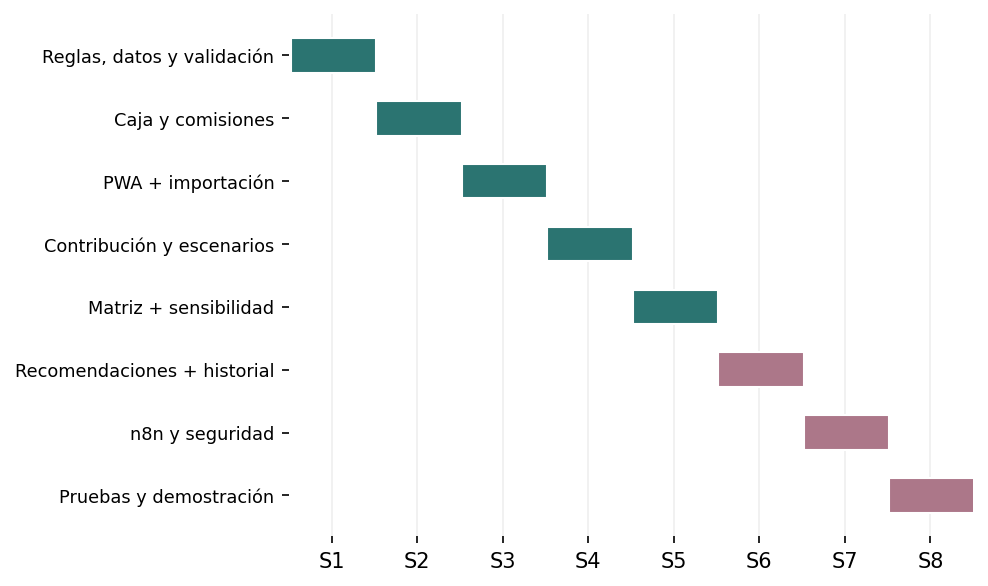
\includegraphics[width=0.9\linewidth]{img/fig_gantt_8sem.png}
\end{figure}

\subsubsection{Hitos y condiciones de salida}

\begin{vinetas}
\item S1: confirmar reglas, costos variables, casos de prueba, procedencia y restricciones de datos.
\item S2: asegurar motor de caja, ventas, cierres, comisiones y liquidación auditables.
\item S3: completar PWA offline e importación asistida con revisión humana.
\item S4: implementar contribución por servicio y escenarios What-If con cálculos de referencia.
\item S5: construir matriz multicriterio, ponderación, reglas de exclusión y sensibilidad.
\item S6: incorporar recomendaciones explicables, aprobación y seguimiento de decisiones.
\item S7: conectar notificaciones n8n a eventos aprobados y completar pruebas de permisos y seguridad.
\item S8: validar tareas decisionales, preparar datos sintéticos, documentar evidencia y ensayar demostración.
\end{vinetas}

\subsection{Guion de demostración ante el jurado}

La demostración ante el jurado seguirá una decisión central: ¿conviene aplicar una promoción del 10~\%? (1) Se muestra el Excel original con servicios inconsistentes; (2) se importa y valida información; (3) se registra una venta offline y se sincroniza sin duplicados; (4) el tablero calcula ingresos, comisiones y contribución; (5) el operador abre tres escenarios What-If y observa el volumen necesario para compensar el descuento; (6) Lush Decision Studio compara alternativas con criterios y sensibilidad; (7) Lush Insight explica la recomendación con evidencias y límites; y (8) la administradora aprueba o rechaza la propuesta y registra una revisión posterior. Como cierre opcional se muestra n8n generando una notificación de decisión aprobada, nunca una modificación automática de pagos.


\subsection{Riesgos y mitigaciones}

\vspace{8pt}{\small\setstretch{1.0}
\begin{longtable}{>{\raggedright\arraybackslash}p{0.3333\dimexpr\linewidth-6\tabcolsep\relax}>{\raggedright\arraybackslash}p{0.3333\dimexpr\linewidth-6\tabcolsep\relax}>{\raggedright\arraybackslash}p{0.3333\dimexpr\linewidth-6\tabcolsep\relax}}
\caption{Riesgos principales de la ampliación y acciones preventivas}\label{tab:dss_8}\\
\toprule
\textbf{Riesgo} & \textbf{Impacto} & \textbf{Tratamiento propuesto} \\
\midrule\endfirsthead
\toprule
\textbf{Riesgo} & \textbf{Impacto} & \textbf{Tratamiento propuesto} \\
\midrule\endhead
\bottomrule\endfoot
\bottomrule\endlastfoot
Alcance excesivo & MVP incompleto & Bloquear alcance crítico y priorizar vertical funcional \\
Pocos datos para ML & Predicciones inestables & Reglas primero; ML etiquetado experimental \\
LLM inventa cifras & Decisiones equivocadas & Herramientas cerradas, sin escritura, pruebas de referencia \\
Pérdida de conectividad & Ventas pendientes & Cola local, idempotencia y recuperación manual \\
Datos de nómina expuestos & Daño reputacional & Permisos, datos sintéticos, enlaces efímeros \\
Fallo de automatización & Avisos no entregados & Outbox, reintentos y seguimiento de errores \\
Cálculo de comisión ambiguo & Diferencia de liquidación & Firma/aprobación de políticas y snapshots \\
Tiempo limitado de feria & Demostración interrumpida & Entorno local, guion, contingencia y registro de video \\
Confundir simulación con predicción & Medio & Rotular supuestos, separar datos observados e hipótesis de volumen. \\
Recomendaciones por pesos arbitrarios & Medio & Validar pesos con administradora y mostrar sensibilidad. \\
Falta de costos de materiales & Medio & Mostrar contribución parcial y marcar faltantes; no afirmar utilidad neta. \\
Demasiados módulos DSS & Medio & Priorizar un solo caso de decisión completo con pruebas. \\
\end{longtable}}

\subsection{Estrategia de recorte y definición de terminado}

Si el tiempo disponible no permite terminar todas las funciones, se protegerá el ciclo de decisión completo: (a) exactitud del núcleo financiero; (b) cálculo de contribución; (c) simulación de tres escenarios; (d) matriz ponderada con sensibilidad y supuestos visibles; (e) recomendación explicable y aprobación humana; (f) historial de decisiones; (g) registro móvil, importación y un flujo n8n que apoyen la demostración. La IA generativa avanzada, las predicciones con ML y la optimización de capacidad podrán aplazarse. Una funcionalidad estará terminada solo cuando incluya interfaz usable, validación en backend, control de permisos, pruebas reproducibles y documentación suficiente para explicarla al jurado.


\section{Conclusiones y Recomendaciones}\label{cap:conclusiones}

\subsection{Conclusiones}

Lush Beauty Smart DSS transforma una propuesta de digitalización de caja y nómina en un sistema de soporte para decisiones sin abandonar el caso empresarial que le da sentido. El aporte distintivo radica en conectar datos operativos con modelos de contribución, escenarios What-If, comparación multicriterio, análisis de sensibilidad, explicaciones y seguimiento. Los resultados de una simulación dependen de sus supuestos, y la aprobación final permanece en manos de la administradora.

Al 26 de noviembre de 2026 el núcleo transaccional está construido y verificado (Capítulo~\ref{cap:implementacion}): el backend pasa 295 pruebas sobre PostgreSQL, la aplicación web 120 y la móvil 32. La Tabla~\ref{tab:concl_1} relaciona ese avance con los objetivos específicos (Capítulo~\ref{cap:objetivos}).

\vspace{8pt}{\small\setstretch{1.0}
\begin{longtable}{>{\raggedright\arraybackslash}p{0.34\linewidth}>{\raggedright\arraybackslash}p{0.15\linewidth}>{\raggedright\arraybackslash}p{0.43\linewidth}}
\caption{Estado de los objetivos específicos}\label{tab:concl_1}\\
\toprule
\textbf{Objetivo específico} & \textbf{Estado} & \textbf{Evidencia o pendiente} \\
\midrule\endfirsthead
\toprule
\textbf{Objetivo específico} & \textbf{Estado} & \textbf{Evidencia o pendiente} \\
\midrule\endhead
\bottomrule\endfoot
\bottomrule\endlastfoot
Describir el proceso actual e identificar inconsistencias de la planilla & Documentado & Capítulo~\ref{cap:problema}; la cuantificación del impacto depende de registros reales anonimizados. \\
Comparar sistemas similares & Cumplido & Capítulo~\ref{cap:benchmarking}. \\
Establecer requisitos, datos y arquitectura & Cumplido & Capítulo~\ref{cap:arquitectura} y esquema de base de datos implementado. \\
Núcleo transaccional con decimal, reglas versionadas, roles y auditoría & Cumplido en backend & Ventas, comisiones, caja y nómina con RLS y auditoría; la interfaz aún no lo consume por completo. \\
PWA con registro sin conexión y sin duplicados & Parcial & Idempotencia por UUID probada; faltan cola local y sincronizador. \\
Importador de Excel & Pendiente & Sin backend; esquema listo. \\
Lush Insight & Pendiente & Sin proveedor de IA ni backend. \\
Lush Guard & Pendiente & Reglas definidas; sin implementación. \\
Automatización con n8n & Parcial & Eventos de cierre y liquidación en la bandeja de salida; faltan los flujos. \\
Modelo de contribución y simulador What-If & Parcial & Falta la vigencia del costo y el simulador. \\
Decision Studio, motor de recomendación y registro de decisiones & Pendiente & Diseñado en el Capítulo~\ref{cap:decision}; sin backend. \\
Evaluar el efecto y la calidad de las decisiones & Pendiente & Requiere pilotaje y mediciones posteriores. \\
\end{longtable}}
\nota{Elaboración propia con base en el Capítulo~\ref{cap:implementacion} y en el backlog del repositorio.}

Se concluye, por tanto, que la parte de caja y nómina cumple su finalidad técnica y es defendible ante el jurado como sistema funcional en el servidor. Las hipótesis sobre reducción de tiempo y de errores, y sobre la utilidad del soporte para decisiones, \textbf{no están contrastadas}: el proyecto cuenta con diseño e instrumentos para hacerlo, pero aún no con mediciones.

La contribución de inteligencia artificial debe ser explicable y limitada: puede ayudar a reconocer nombres inconsistentes, recuperar información autorizada y redactar resúmenes; no puede establecer pagos ni crear cifras económicas por inferencia. Las alertas estadísticas y el machine learning deberán permanecer como experimentos hasta contar con historial suficiente y evaluación contra casos etiquetados. La automatización también estará sometida a eventos aprobados y a mecanismos de seguridad, reintento y auditoría.

\subsection{Limitaciones}

Las principales limitaciones son tres: la interfaz permanece mayormente en maqueta sin conectar al API; el módulo de decisiones no tiene backend, de modo que el ciclo completo de decisión exigido por los criterios de aceptación globales aún no es reproducible; y varias reglas de negocio operan con valores provisionales sin validar con la administradora. Además, no se ha medido cobertura de código, carga ni conexión intermitente.

\subsection{Recomendaciones}

Se recomienda, en este orden: (1) conectar la interfaz a los endpoints ya existentes de ventas, caja, comisiones y nómina para eliminar las maquetas; (2) construir primero un ciclo completo de decisión reproducible (contribución, tres escenarios, matriz, sensibilidad, recomendación y aprobación humana), que es el eje protegido del proyecto; (3) validar con la administradora las reglas de comisiones, costos directos, redondeo, umbral de descuento, semana de liquidación y los criterios y pesos de decisión; (4) obtener registros reales anonimizados para la línea base; y (5) fijar la fecha de presentación. Si el tiempo no alcanza, se aplazarán la IA generativa avanzada, el aprendizaje automático y la optimización, y se mantendrá un único flujo mínimo de n8n.

Los resultados de desempeño, aceptación e impacto económico se documentarán únicamente cuando existan mediciones posteriores. La meta académica es demostrar utilidad de decisión y calidad metodológica, no solo complejidad tecnológica.

\section{Referencias}\label{cap:referencias}

\referencia{AgendaPro. (s. f.). \textit{Software de agenda y gestión para negocios de belleza}. Recuperado el 30 de octubre de 2026, de \url{https://agendapro.com}}
\referencia{Bezemer, C.-P., \& Zaidman, A. (2010). Multi-tenant SaaS applications: Maintenance dream or nightmare? En \textit{Proceedings of the Joint ERCIM Workshop on Software Evolution (EVOL) and International Workshop on Principles of Software Evolution (IWPSE)} (pp. 88–92). ACM. \url{https://doi.org/10.1145/1862372.1862393}}
\referencia{Booksy. (s. f.). \textit{Booksy Biz: Software para salones, barberías y negocios de belleza}. Recuperado el 30 de octubre de 2026, de \url{https://biz.booksy.com/en-us}}
\referencia{Brooke, J. (1996). SUS: A “quick and dirty” usability scale. En P. W. Jordan, B. Thomas, B. A. Weerdmeester, \& I. L. McClelland (Eds.), \textit{Usability evaluation in industry} (pp. 189–194). Taylor \& Francis.}
\referencia{Camp, R. C. (1989). \textit{Benchmarking: The search for industry best practices that lead to superior performance}. ASQC Quality Press.}
\referencia{Cronbach, L. J. (1951). Coefficient alpha and the internal structure of tests. \textit{Psychometrika, 16}(3), 297–334. \url{https://doi.org/10.1007/BF02310555}}
\referencia{Davis, F. D. (1989). Perceived usefulness, perceived ease of use, and user acceptance of information technology. \textit{MIS Quarterly, 13}(3), 319–340. \url{https://doi.org/10.2307/249008}}
\referencia{DeLone, W. H., \& McLean, E. R. (2003). The DeLone and McLean model of information systems success: A ten-year update. \textit{Journal of Management Information Systems, 19}(4), 9–30. \url{https://doi.org/10.1080/07421222.2003.11045748}}
\referencia{Django Software Foundation. (s. f.-a). \textit{Database transactions}. Django documentation. \url{https://docs.djangoproject.com/en/5.2/topics/db/transactions/}}
\referencia{Django Software Foundation. (s. f.-b). \textit{Model field reference}. Django documentation. \url{https://docs.djangoproject.com/en/5.2/ref/models/fields/}}
\referencia{Expo. (s. f.). \textit{Core concepts}. Expo documentation. \url{https://docs.expo.dev/core-concepts/}}
\referencia{Fresha. (s. f.). \textit{Fresha for business: Salon and spa software}. Recuperado el 30 de octubre de 2026, de \url{https://www.fresha.com/for-business}}
\referencia{Hernández Sampieri, R., Fernández Collado, C., \& Baptista Lucio, P. (2014). \textit{Metodología de la investigación} (6.ª ed.). McGraw-Hill.}
\referencia{Hevner, A. R., March, S. T., Park, J., \& Ram, S. (2004). Design science in information systems research. \textit{MIS Quarterly, 28}(1), 75–105. \url{https://aisel.aisnet.org/misq/vol28/iss1/6/}}
\referencia{HM Treasury. (s. f.). \textit{Use of multi-criteria decision analysis in options appraisal of economic cases}. GOV.UK. \url{https://www.gov.uk/government/publications/green-book-supplementary-guidance-multi-criteria-decision-analysis/use-of-multi-criteria-decision-analysis-in-options-appraisal-of-economic-cases}}
\referencia{International Organization for Standardization \& International Electrotechnical Commission. (2011). \textit{Systems and software engineering — Systems and software quality requirements and evaluation (SQuaRE) — System and software quality models} (ISO/IEC 25010:2011). ISO.}
\referencia{Laudon, K. C., \& Laudon, J. P. (2016). \textit{Sistemas de información gerencial} (14.ª ed.). Pearson Educación.}
\referencia{Meré Espino, R. (2016). \textit{Web para el sitio y gestión de un salón de belleza} [Proyecto fin de carrera, Universidad de Las Palmas de Gran Canaria]. Repositorio institucional ULPGC. \url{https://accedacris.ulpgc.es/handle/10553/17707}}
\referencia{Mozilla Developer Network. (s. f.-a). \textit{Offline and background operation — Progressive web apps}. \url{https://developer.mozilla.org/en-US/docs/Web/Progressive_web_apps/Guides/Offline_and_background_operation}}
\referencia{Mozilla Developer Network. (s. f.-b). \textit{Using IndexedDB}. \url{https://developer.mozilla.org/en-US/docs/Web/API/IndexedDB_API/Using_IndexedDB}}
\referencia{n8n. (s. f.). \textit{n8n documentation}. \url{https://docs.n8n.io/}}
\referencia{National Institute of Standards and Technology. (2023). \textit{Artificial Intelligence Risk Management Framework (AI RMF 1.0)}. \url{https://doi.org/10.6028/NIST.AI.100-1}}
\referencia{Ochoa López, D. E. (2021). \textit{Sistema web para la gestión de la administración de la peluquería y estética del salón de belleza Mónica Garcés} [Propuesta tecnológica, Universidad Agraria del Ecuador]. Repositorio institucional de la Universidad Agraria del Ecuador. \url{https://cia.uagraria.edu.ec/Archivos/OCHOA\%20LOPEZ\%20DAYANNA\%20ELIZABETH.pdf}}
\referencia{Panko, R. R. (1998). What we know about spreadsheet errors. \textit{Journal of End User Computing, 10}(2), 15–21.}
\referencia{React. (s. f.). \textit{Using TypeScript}. React documentation. \url{https://react.dev/learn/typescript}}
\referencia{Schwaber, K., \& Sutherland, J. (2020). \textit{The Scrum Guide}. \url{https://scrumguides.org/scrum-guide.html}}
\referencia{scikit-learn Developers. (s. f.-a). \textit{IsolationForest}. scikit-learn documentation. \url{https://scikit-learn.org/stable/modules/generated/sklearn.ensemble.IsolationForest.html}}
\referencia{scikit-learn Developers. (s. f.-b). \textit{TimeSeriesSplit}. scikit-learn documentation. \url{https://scikit-learn.org/stable/modules/generated/sklearn.model_selection.TimeSeriesSplit.html}}
\referencia{SciPy Community. (s. f.). \textit{scipy.optimize.linprog}. SciPy documentation. \url{https://docs.scipy.org/doc/scipy/reference/generated/scipy.optimize.linprog.html}}
\referencia{Sommerville, I. (2011). \textit{Ingeniería de software} (9.ª ed.). Pearson Educación.}
\referencia{Vagaro. (s. f.). \textit{Salon software}. Recuperado el 30 de octubre de 2026, de \url{https://www.vagaro.com/pro/salon-software}}
\referencia{Wroblewski, L. (2011). \textit{Mobile first}. A Book Apart.}

\section{Anexos}\label{cap:anexos}

Los anexos contienen los instrumentos de recolección de datos y los formatos de consentimiento. Todos se aplicarán después de su validación por juicio de expertos. Los anexos A a G corresponden a los instrumentos de recolección de datos y a los formatos del estudio; los anexos H a Q reúnen la documentación técnica y de evaluación de la ampliación Lush Beauty Smart DSS (requisitos, historias de usuario, casos de prueba, diseño de API y de flujos n8n, instrumentos adicionales, lista de preparación, fichas de decisión y evaluación de decisiones).

\anexotabla{A}

\anexo{Anexo A. Cuestionario de requerimientos}

Cuestionario de requerimientos del sistema de gestión del salón Lush Beauty. Está dirigido a la administradora y a las especialistas, con una duración estimada de 25 minutos. No existen respuestas correctas; se solicita describir la operación actual del salón con la mayor precisión posible.


\textbf{Instrucciones:} marque con una X las opciones indicadas o escriba en los espacios previstos. Sus respuestas son confidenciales y se identifican con un código de participante. En el Anexo G se presenta un ejemplo de llenado.


Código de participante: \blank{8}     Fecha: \blank{4}/\blank{4}/\blank{8}


\subanexo{I. Datos generales}

\pregunta{\textbf{1.} Su rol en el salón:}

\opciones{[~~] Administración\quad{}[~~] Especialista\quad{}[~~] Ambos}

\pregunta{\textbf{2.} ¿Cuántos años lleva operando el salón? \blank{12}}

\pregunta{\textbf{3.} ¿Cuántas personas prestan servicios actualmente? \blank{12}}

\pregunta{\textbf{4.} ¿Cuántos servicios se realizan en un día habitual? \blank{12}}

\pregunta{\textbf{5.} ¿Con qué dispositivos se registran hoy los servicios?}

\opciones{[~~] Celular\quad{}[~~] Computadora\quad{}[~~] Papel\quad{}[~~] Hoja de cálculo\quad{}[~~] Otro: \blank{8}}

\subanexo{II. Registro de servicios y caja}

\pregunta{\textbf{6.} ¿Cómo registra hoy los servicios realizados?}

\opciones{[~~] Libreta\quad{}[~~] Hoja de cálculo\quad{}[~~] Mensajes\quad{}[~~] Otro: \blank{8}}

\pregunta{\textbf{7.} ¿Cuándo registra un servicio?}

\opciones{[~~] En el momento\quad{}[~~] Al final del día\quad{}[~~] Al final de la semana}

\pregunta{\textbf{8.} Marque los datos que registra por cada servicio:}

\opciones{[~~] Fecha\quad{}[~~] Hora\quad{}[~~] Cliente\quad{}[~~] Especialista\quad{}[~~] Servicio\quad{}[~~] Precio\quad{}[~~] Descuento\quad{}[~~] Método de pago\quad{}[~~] Propina\quad{}[~~] Observaciones}

\pregunta{\textbf{9.} ¿Qué métodos de pago acepta?}

\opciones{[~~] Efectivo\quad{}[~~] QR\quad{}[~~] Transferencia\quad{}[~~] Tarjeta\quad{}[~~] Otro: \blank{8}}

\pregunta{\textbf{10.} ¿Un cliente puede pagar varios servicios en un mismo cobro (combos)?}

\opciones{[~~] Sí, frecuentemente\quad{}[~~] Sí, a veces\quad{}[~~] No}

\pregunta{\textbf{11.} ¿Cómo cuadra la caja al cierre del día? \blank{46}}

\pregunta{\textbf{12.} ¿Qué descuentos aplica y quién los autoriza?}

\opciones{[~~] Porcentaje fijo\quad{}[~~] Monto fijo\quad{}[~~] Libre}

\pregunta{\textbf{13.} Cuando un servicio se cancela, ¿qué sucede con el registro y con la comisión? \blank{30}}

\subanexo{III. Comisiones y liquidación}

\pregunta{\textbf{14.} ¿Qué porcentaje de comisión recibe cada especialista? \blank{12}}

\pregunta{\textbf{15.} ¿Sobre qué monto se calcula la comisión?}

\opciones{[~~] Precio de lista\quad{}[~~] Monto cobrado\quad{}[~~] Otro: \blank{8}}

\pregunta{\textbf{16.} ¿La comisión cambia según el servicio, la categoría o la persona?}

\opciones{[~~] Sí\quad{}[~~] No}

\pregunta{\textbf{17.} Explique la respuesta anterior, si corresponde: \blank{46}}

\pregunta{\textbf{18.} ¿Cada cuánto tiempo se paga al personal?}

\opciones{[~~] Semanal\quad{}[~~] Quincenal\quad{}[~~] Mensual\quad{}[~~] Otro: \blank{8}}

\pregunta{\textbf{19.} ¿Existe un sueldo fijo además de la comisión?}

\opciones{[~~] Sí, monto: \blank{8}\quad{}[~~] No}

\pregunta{\textbf{20.} ¿Qué deducciones se aplican al personal, y cómo se calcula cada una?}

\opciones{[~~] Adelantos\quad{}[~~] Faltas\quad{}[~~] Materiales\quad{}[~~] Otras: \blank{8}}

\pregunta{\textbf{21.} ¿Qué sucede cuando las deducciones superan lo ganado en el periodo? \blank{30}}

\pregunta{\textbf{22.} ¿Cómo se entrega el pago y su detalle al personal?}

\opciones{[~~] Efectivo sin detalle\quad{}[~~] Efectivo con detalle impreso\quad{}[~~] Mensaje\quad{}[~~] Otro: \blank{8}}

\subanexo{IV. Propinas}

\pregunta{\textbf{23.} ¿Cómo se registran hoy las propinas? \blank{30}}

\pregunta{\textbf{24.} ¿Cómo se reparten las propinas?}

\opciones{[~~] 100~\% a quien atendió\quad{}[~~] Entre el equipo\quad{}[~~] Con retención del salón\quad{}[~~] Otro: \blank{8}}

\pregunta{\textbf{25.} ¿Necesita modificar una propina después de registrada?}

\opciones{[~~] Sí\quad{}[~~] No}

\subanexo{V. Clientes}

\pregunta{\textbf{26.} ¿Cómo lleva el registro de clientes?}

\opciones{[~~] No lo lleva\quad{}[~~] Libreta\quad{}[~~] Hoja de cálculo\quad{}[~~] Otro: \blank{8}}

\pregunta{\textbf{27.} ¿Qué datos necesita de cada clienta?}

\opciones{[~~] Nombre\quad{}[~~] Teléfono\quad{}[~~] Fecha de nacimiento\quad{}[~~] Preferencias\quad{}[~~] Notas\quad{}[~~] Otros: \blank{8}}

\pregunta{\textbf{28.} ¿Necesita ver el historial de servicios de una clienta?}

\opciones{[~~] Sí\quad{}[~~] No}

\pregunta{\textbf{29.} ¿Ha tenido dificultades con nombres duplicados o confusos? Describa: \blank{30}}

\subanexo{VI. Catálogo y precios}

\pregunta{\textbf{30.} ¿Con qué frecuencia cambian los precios? \blank{12}}

\pregunta{\textbf{31.} ¿Hay servicios cuyo precio varía al momento del cobro (por ejemplo, diseños)? Cuáles: \blank{30}}

\opciones{[~~] Sí\quad{}[~~] No}

\pregunta{\textbf{32.} ¿Quién debe poder modificar el catálogo y los precios? \blank{12}}

\subanexo{VII. Reportes, importación y exportación}

\pregunta{\textbf{33.} ¿Qué reportes necesita?}

\opciones{[~~] Caja diaria\quad{}[~~] Detalle por servicio\quad{}[~~] Liquidación por persona\quad{}[~~] Otros: \blank{8}}

\pregunta{\textbf{34.} ¿En qué formato los necesita?}

\opciones{[~~] Excel\quad{}[~~] PDF\quad{}[~~] Pantalla\quad{}[~~] Otro: \blank{8}}

\pregunta{\textbf{35.} ¿Necesita trasladar a la nueva herramienta la información de su planilla actual?}

\opciones{[~~] Sí\quad{}[~~] No}

\pregunta{\textbf{36.} ¿Quién necesita recibir reportes fuera del salón?}

\opciones{[~~] Contador\quad{}[~~] Familia o socios\quad{}[~~] Ninguno\quad{}[~~] Otro: \blank{8}}

\subanexo{VIII. Uso, conectividad y seguridad}

\pregunta{\textbf{37.} ¿Con qué frecuencia se queda sin internet mientras atiende?}

\opciones{[~~] Nunca\quad{}[~~] Pocas veces al mes\quad{}[~~] Casi a diario}

\pregunta{\textbf{38.} ¿Necesita registrar servicios cuando no hay internet?}

\opciones{[~~] Sí\quad{}[~~] No}

\pregunta{\textbf{39.} ¿Quién debe poder ver los sueldos y las comisiones? \blank{12}}

\pregunta{\textbf{40.} ¿Quién debe poder modificar o eliminar un registro? \blank{12}}

\pregunta{\textbf{41.} ¿Necesita saber quién cambió un dato, cuándo y cuál era el valor anterior?}

\opciones{[~~] Sí\quad{}[~~] No}

\subanexo{IX. Priorización de necesidades}

\pregunta{\textbf{42.} Califique cada necesidad del 1 (no es importante) al 5 (imprescindible), marcando una casilla por fila.}

\vspace{8pt}{\footnotesize\setstretch{1.0}
\begin{longtable}{>{\raggedright\arraybackslash}p{0.6251\dimexpr\linewidth-12\tabcolsep\relax}>{\raggedright\arraybackslash}p{0.0750\dimexpr\linewidth-12\tabcolsep\relax}>{\raggedright\arraybackslash}p{0.0750\dimexpr\linewidth-12\tabcolsep\relax}>{\raggedright\arraybackslash}p{0.0750\dimexpr\linewidth-12\tabcolsep\relax}>{\raggedright\arraybackslash}p{0.0750\dimexpr\linewidth-12\tabcolsep\relax}>{\raggedright\arraybackslash}p{0.0750\dimexpr\linewidth-12\tabcolsep\relax}}
\caption{Priorización de necesidades del salón}\label{tab:v4_A1}\\
\toprule
\textbf{Necesidad} & \textbf{1} & \textbf{2} & \textbf{3} & \textbf{4} & \textbf{5} \\
\midrule\endfirsthead
\toprule
\textbf{Necesidad} & \textbf{1} & \textbf{2} & \textbf{3} & \textbf{4} & \textbf{5} \\
\midrule\endhead
\bottomrule\endfoot
\bottomrule\endlastfoot
Registrar un servicio en menos de 15 segundos desde el celular &  &  &  &  &  \\
Calcular automáticamente la comisión de cada línea &  &  &  &  &  \\
Liquidación semanal con deducciones y excedentes &  &  &  &  &  \\
Comprobante en PDF para compartir por WhatsApp &  &  &  &  &  \\
Registrar servicios sin conexión a internet &  &  &  &  &  \\
Importar la planilla actual de Excel &  &  &  &  &  \\
Bitácora de cambios consultable &  &  &  &  &  \\
Reportes en Excel para el contador &  &  &  &  &  \\
Ficha de clientes con historial &  &  &  &  &  \\
Agenda de citas en línea (posible etapa posterior) &  &  &  &  &  \\
\end{longtable}}

\subanexo{X. Observaciones}

\pregunta{\textbf{43.} ¿Cuál es el problema que más le preocupa hoy en la gestión del salón? \blank{30}}

\pregunta{\textbf{44.} ¿Qué parte del proceso actual no debería cambiar? \blank{30}}

Gracias por su participación.


\anexotabla{B}

\anexo{Anexo B. Cuestionario de usabilidad (SUS, versión en español)}

Versión en español del \textit{System Usability Scale} (Brooke, 1996). La traducción es propia y debe validarse por juicio de expertos antes de su aplicación. Se responde después de usar el sistema durante el piloto. Escala: 1 = totalmente en desacuerdo; 5 = totalmente de acuerdo.


\pregunta{\textbf{1.} Creo que me gustaría usar este sistema con frecuencia.}

\opciones{[~~] 1\quad{}[~~] 2\quad{}[~~] 3\quad{}[~~] 4\quad{}[~~] 5}

\pregunta{\textbf{2.} Encontré el sistema innecesariamente complejo.}

\opciones{[~~] 1\quad{}[~~] 2\quad{}[~~] 3\quad{}[~~] 4\quad{}[~~] 5}

\pregunta{\textbf{3.} Pensé que el sistema era fácil de usar.}

\opciones{[~~] 1\quad{}[~~] 2\quad{}[~~] 3\quad{}[~~] 4\quad{}[~~] 5}

\pregunta{\textbf{4.} Creo que necesitaría el apoyo de una persona técnica para poder usar este sistema.}

\opciones{[~~] 1\quad{}[~~] 2\quad{}[~~] 3\quad{}[~~] 4\quad{}[~~] 5}

\pregunta{\textbf{5.} Encontré que las distintas funciones del sistema estaban bien integradas.}

\opciones{[~~] 1\quad{}[~~] 2\quad{}[~~] 3\quad{}[~~] 4\quad{}[~~] 5}

\pregunta{\textbf{6.} Pensé que había demasiadas inconsistencias en este sistema.}

\opciones{[~~] 1\quad{}[~~] 2\quad{}[~~] 3\quad{}[~~] 4\quad{}[~~] 5}

\pregunta{\textbf{7.} Imagino que la mayoría de las personas aprendería a usar este sistema muy rápidamente.}

\opciones{[~~] 1\quad{}[~~] 2\quad{}[~~] 3\quad{}[~~] 4\quad{}[~~] 5}

\pregunta{\textbf{8.} Encontré el sistema muy incómodo de usar.}

\opciones{[~~] 1\quad{}[~~] 2\quad{}[~~] 3\quad{}[~~] 4\quad{}[~~] 5}

\pregunta{\textbf{9.} Me sentí muy seguro al usar el sistema.}

\opciones{[~~] 1\quad{}[~~] 2\quad{}[~~] 3\quad{}[~~] 4\quad{}[~~] 5}

\pregunta{\textbf{10.} Necesité aprender muchas cosas antes de poder empezar a usar este sistema.}

\opciones{[~~] 1\quad{}[~~] 2\quad{}[~~] 3\quad{}[~~] 4\quad{}[~~] 5}

\textbf{Cálculo de la puntuación.} En los ítems impares se resta 1 a la respuesta; en los pares, la respuesta se resta de 5. La suma de los valores obtenidos se multiplica por 2,5, lo que da un resultado entre 0 y 100.


\anexotabla{C}

\anexo{Anexo C. Fichas de observación y de conciliación}



\subanexo{C.1 Ficha de observación cronometrada}

\vspace{8pt}{\footnotesize\setstretch{1.0}
\begin{longtable}{>{\raggedright\arraybackslash}p{0.1150\dimexpr\linewidth-14\tabcolsep\relax}>{\raggedright\arraybackslash}p{0.2414\dimexpr\linewidth-14\tabcolsep\relax}>{\raggedright\arraybackslash}p{0.0920\dimexpr\linewidth-14\tabcolsep\relax}>{\raggedright\arraybackslash}p{0.0920\dimexpr\linewidth-14\tabcolsep\relax}>{\raggedright\arraybackslash}p{0.1034\dimexpr\linewidth-14\tabcolsep\relax}>{\raggedright\arraybackslash}p{0.1724\dimexpr\linewidth-14\tabcolsep\relax}>{\raggedright\arraybackslash}p{0.1839\dimexpr\linewidth-14\tabcolsep\relax}}
\caption{Registro de tiempos de los procesos observados}\label{tab:v4_C1}\\
\toprule
\textbf{Fecha} & \textbf{Actividad} & \textbf{Inicio} & \textbf{Fin} & \textbf{Duración} & \textbf{Errores o reprocesos} & \textbf{Observaciones} \\
\midrule\endfirsthead
\toprule
\textbf{Fecha} & \textbf{Actividad} & \textbf{Inicio} & \textbf{Fin} & \textbf{Duración} & \textbf{Errores o reprocesos} & \textbf{Observaciones} \\
\midrule\endhead
\bottomrule\endfoot
\bottomrule\endlastfoot
 & Registro de servicio / Cierre de caja / Liquidación &  &  &  &  &  \\
 & Registro de servicio / Cierre de caja / Liquidación &  &  &  &  &  \\
 & Registro de servicio / Cierre de caja / Liquidación &  &  &  &  &  \\
\end{longtable}}

\subanexo{C.2 Ficha de conciliación de cálculos}

\vspace{8pt}{\small\setstretch{1.0}
\begin{longtable}{>{\raggedright\arraybackslash}p{0.1905\dimexpr\linewidth-10\tabcolsep\relax}>{\raggedright\arraybackslash}p{0.2262\dimexpr\linewidth-10\tabcolsep\relax}>{\raggedright\arraybackslash}p{0.2262\dimexpr\linewidth-10\tabcolsep\relax}>{\raggedright\arraybackslash}p{0.1786\dimexpr\linewidth-10\tabcolsep\relax}>{\raggedright\arraybackslash}p{0.1786\dimexpr\linewidth-10\tabcolsep\relax}}
\caption{Comparación de comisiones calculadas por el sistema y por el cálculo de referencia}\label{tab:v4_C2}\\
\toprule
\textbf{Registro} & \textbf{Comisión del sistema (Bs)} & \textbf{Comisión de referencia (Bs)} & \textbf{Diferencia (Bs)} & \textbf{Coincide (sí/no)} \\
\midrule\endfirsthead
\toprule
\textbf{Registro} & \textbf{Comisión del sistema (Bs)} & \textbf{Comisión de referencia (Bs)} & \textbf{Diferencia (Bs)} & \textbf{Coincide (sí/no)} \\
\midrule\endhead
\bottomrule\endfoot
\bottomrule\endlastfoot
 &  &  &  &  \\
 &  &  &  &  \\
 &  &  &  &  \\
\end{longtable}}

\anexotabla{D}

\anexo{Anexo D. Guía de entrevista semiestructurada}

Entrevista dirigida a la administradora, con una duración aproximada de 30 a 40 minutos. Se grabará únicamente con su consentimiento (Anexo E).


\pregunta{\textbf{1.} ¿Cómo describe el funcionamiento diario del salón, desde que llega una clienta hasta que se cobra el servicio?}

\pregunta{\textbf{2.} ¿Qué parte del proceso le toma más tiempo o le genera más preocupación?}

\pregunta{\textbf{3.} ¿Qué situaciones le han generado errores o diferencias en la caja o en las comisiones?}

\pregunta{\textbf{4.} ¿Cómo calcula y paga la liquidación semanal? ¿Qué parte le resulta más difícil?}

\pregunta{\textbf{5.} ¿Qué opina de registrar los servicios desde el celular durante la jornada?}

\pregunta{\textbf{6.} ¿Qué expectativas tiene sobre un sistema que reemplace la planilla?}

\pregunta{\textbf{7.} ¿Qué condiciones considera indispensables para dejar de usar la planilla?}

\pregunta{\textbf{8.} ¿Qué aspecto de la planilla actual no debería perderse en el nuevo sistema?}

\anexotabla{E}

\anexo{Anexo E. Formato de consentimiento informado}

Usted está invitada a participar en el trabajo final de investigación «Sistema Web Móvil para la Gestión de Caja y Nómina del Salón de Belleza Lush Beauty». Su participación consiste en responder un cuestionario, participar en una entrevista y, si corresponde, usar el sistema durante el piloto.


La participación es voluntaria y puede retirarse en cualquier momento, sin consecuencias. La información se utilizará solo con fines académicos. Los datos de sueldos y de clientes se tratarán de forma confidencial y se presentarán de manera agregada o con códigos.


Nombre: \blank{30}     Firma: \blank{22}     Fecha: \blank{4}/\blank{4}/\blank{8}


\anexotabla{F}

\anexo{Anexo F. Planilla de ejemplo anonimizada}

Captura de la planilla de ejemplo de agosto de 2026, con los nombres de clientes sustituidos por códigos. [Insertar imagen anonimizada.]


\anexotabla{G}

\anexo{Anexo G. Ejemplo de cuestionario de requerimientos respondido}

\textbf{Ejemplo ilustrativo.} Las respuestas siguientes no provienen de una aplicación real del cuestionario. Se construyeron a partir de la información disponible en el documento de definición del producto (PDR) del proyecto y de la planilla de ejemplo de agosto de 2026. Las respuestas marcadas como «[por confirmar]» deben completarse con la administradora antes de utilizar el cuestionario como fuente de datos.


\vspace{8pt}{\small\setstretch{1.0}
\begin{longtable}{>{\raggedright\arraybackslash}p{0.0692\dimexpr\linewidth-6\tabcolsep\relax}>{\raggedright\arraybackslash}p{0.3522\dimexpr\linewidth-6\tabcolsep\relax}>{\raggedright\arraybackslash}p{0.5786\dimexpr\linewidth-6\tabcolsep\relax}}
\caption{Respuestas ilustrativas al cuestionario de requerimientos}\label{tab:v4_G1}\\
\toprule
\textbf{N.º} & \textbf{Pregunta (resumida)} & \textbf{Respuesta ilustrativa} \\
\midrule\endfirsthead
\toprule
\textbf{N.º} & \textbf{Pregunta (resumida)} & \textbf{Respuesta ilustrativa} \\
\midrule\endhead
\bottomrule\endfoot
\bottomrule\endlastfoot
1 & Rol en el salón & Ambos (administración y especialista) \\
2 & Años operando el salón & [por confirmar] \\
3 & Personas que prestan servicios & 3 \\
4 & Servicios en un día habitual & Aprox. 3 (91 servicios en agosto de 2026, según la planilla de ejemplo) \\
5 & Dispositivos para registrar & Celular; hoja de cálculo \\
6 & Forma de registro actual & Hoja de cálculo \\
7 & Momento del registro & Al final del día [por confirmar] \\
8 & Datos que registra & Fecha, cliente, especialista, servicio, precio, descuento, propina y observaciones; no registra método de pago \\
9 & Métodos de pago & Efectivo, QR, transferencia y tarjeta [por confirmar] \\
10 & Cobros combinados (combos) & Sí, a veces \\
11 & Cuadre de caja al cierre & Suma manual de montos; no hay desglose por método de pago \\
12 & Descuentos y autorización & Porcentaje fijo (0 a 50~\%); autoriza la administradora \\
13 & Servicio cancelado & [por confirmar] \\
14 & Porcentaje de comisión & 35~\% \\
15 & Base de cálculo de la comisión & Precio de lista \\
16 & La comisión varía & No \\
17 & Explicación & No aplica \\
18 & Frecuencia de pago al personal & Semanal \\
19 & Sueldo fijo además de la comisión & [por confirmar] \\
20 & Deducciones y cálculo & Adelantos, faltas y materiales; monto definido a mano [por confirmar] \\
21 & Deducciones mayores a lo ganado & [por confirmar] \\
22 & Forma de entregar el pago y el detalle & [por confirmar] \\
23 & Registro de propinas & En una columna aparte, sin pasar por la comisión \\
24 & Reparto de propinas & 100~\% a quien atendió [por confirmar] \\
25 & Necesidad de editar propinas & Sí \\
26 & Registro de clientes & Hoja de cálculo, como texto libre \\
27 & Datos de cada clienta & Nombre, teléfono y notas \\
28 & Historial de servicios por clienta & Sí \\
29 & Nombres duplicados o confusos & Sí: nombres con anotaciones y espacios finales \\
30 & Frecuencia de cambio de precios & [por confirmar] \\
31 & Precios que varían al cobro & Sí: diseños (base más Bs~20) y arreglos sin precio publicado \\
32 & Quién modifica catálogo y precios & La administradora \\
33 & Reportes necesarios & Caja diaria, detalle por servicio y liquidación por persona \\
34 & Formato de los reportes & Excel, y PDF para compartir \\
35 & Migrar la planilla actual & Sí \\
36 & Quién recibe reportes fuera del salón & Contador \\
37 & Frecuencia de corte de internet & [por confirmar] \\
38 & Registrar sin internet & Sí \\
39 & Quién ve sueldos y comisiones & Solo la administradora \\
40 & Quién modifica o elimina registros & Solo la administradora \\
41 & Bitácora de cambios & Sí \\
42 & Priorización (1 a 5) & Registro rápido 5; comisión automática 5; liquidación con deducciones 5; PDF para WhatsApp 4; sin conexión 4; importar Excel 4; bitácora 4; reportes para el contador 3; clientes con historial 3; agenda en línea 1 \\
43 & Problema que más preocupa & Errores de cálculo y tiempo de liquidación (ilustrativo) \\
44 & Parte del proceso que no debe cambiar & [por confirmar] \\
\end{longtable}}

\anexotabla{H}

\anexo{Anexo H. Matriz inicial de requisitos funcionales}

Los requisitos siguientes se presentan como propuesta de implementación, y deben validarse mediante entrevistas y revisión técnica antes de convertirse en línea base aprobada.


\vspace{8pt}{\small\setstretch{1.0}
\begin{longtable}{>{\raggedright\arraybackslash}p{0.3333\dimexpr\linewidth-6\tabcolsep\relax}>{\raggedright\arraybackslash}p{0.3333\dimexpr\linewidth-6\tabcolsep\relax}>{\raggedright\arraybackslash}p{0.3333\dimexpr\linewidth-6\tabcolsep\relax}}
\caption{Priorización sugerida; no sustituye las decisiones de las participantes del salón}\label{tab:dss_A1}\\
\toprule
\textbf{Código} & \textbf{Requisito propuesto} & \textbf{Prioridad} \\
\midrule\endfirsthead
\toprule
\textbf{Código} & \textbf{Requisito propuesto} & \textbf{Prioridad} \\
\midrule\endhead
\bottomrule\endfoot
\bottomrule\endlastfoot
RF-01 & Registrar venta con una o varias líneas & Crítica \\
RF-02 & Asignar especialista y servicio del catálogo & Crítica \\
RF-03 & Registrar pago por efectivo, QR o transferencia & Crítica \\
RF-04 & Aplicar descuentos con motivo y aprobación & Crítica \\
RF-05 & Calcular comisión según regla versionada & Crítica \\
RF-06 & Registrar propinas y deducciones & Crítica \\
RF-07 & Generar y aprobar liquidación semanal & Crítica \\
RF-08 & Cerrar y conciliar caja diaria & Crítica \\
RF-09 & Generar comprobantes PDF y exportaciones XLSX & Alta \\
RF-10 & Registrar servicio sin conectividad & Alta \\
RF-11 & Sincronizar idempotentemente operaciones & Crítica \\
RF-12 & Importar y mapear hojas XLSX & Alta \\
RF-13 & Proponer aliases y detectar duplicados & Alta \\
RF-14 & Registrar correcciones y fuentes de importación & Alta \\
RF-15 & Consultar dashboard financiero & Alta \\
RF-16 & Consultar cinco intenciones de Lush Insight & Alta \\
RF-17 & Detectar alertas de reglas Lush Guard & Alta \\
RF-18 & Automatizar tres eventos aprobados con n8n & Alta \\
RF-19 & Aislar permisos y datos de cada salón & Crítica \\
RF-20 & Registrar auditoría y cambios históricos & Crítica \\
\end{longtable}}

\anexo{Anexo I. Historias de usuario para el backlog inicial}

\textbf{HU-01. Como administradora, quiero registrar una venta con servicios y métodos de pago, para gestionar con trazabilidad el proceso.}


\textit{Criterio de aceptación:} el importe de líneas coincide con pagos y se genera detalle.


\textbf{HU-02. Como especialista, quiero registrar un servicio desde el móvil sin internet, para gestionar con trazabilidad el proceso.}


\textit{Criterio de aceptación:} la cola muestra pendiente y luego confirmada sin duplicación.


\textbf{HU-03. Como administradora, quiero establecer una política de comisiones vigente, para gestionar con trazabilidad el proceso.}


\textit{Criterio de aceptación:} el cálculo usa un snapshot histórico y conserva motivo de cambios.


\textbf{HU-04. Como administradora, quiero liquidar una semana con propinas y deducciones, para gestionar con trazabilidad el proceso.}


\textit{Criterio de aceptación:} se obtiene un total verificable y un PDF por especialista.


\textbf{HU-05. Como administradora, quiero importar mi planilla anterior, para gestionar con trazabilidad el proceso.}


\textit{Criterio de aceptación:} recibo un reporte de accepted/reviewed/rejected antes de confirmar.


\textbf{HU-06. Como administradora, quiero consultar por qué cambió el neto, para gestionar con trazabilidad el proceso.}


\textit{Criterio de aceptación:} el asistente consulta el período y muestra la fuente del cálculo.


\textbf{HU-07. Como administradora, quiero recibir una alerta si se supera un umbral, para gestionar con trazabilidad el proceso.}


\textit{Criterio de aceptación:} la alerta indica regla y permite marcar revisión.


\textbf{HU-08. Como administradora, quiero enviar un aviso al aprobar caja, para gestionar con trazabilidad el proceso.}


\textit{Criterio de aceptación:} el flujo n8n registra éxito o fallo y permite reintentar.


\textbf{HU-09. Como especialista, quiero ver mi propia liquidación, para gestionar con trazabilidad el proceso.}


\textit{Criterio de aceptación:} no puedo consultar las de otras especialistas.


\textbf{HU-10. Como administradora, quiero revertir una venta con motivo, para gestionar con trazabilidad el proceso.}


\textit{Criterio de aceptación:} se conserva historial y se genera ajuste correspondiente.


\anexotabla{J}

\anexo{Anexo J. Casos de prueba de aceptación}

\vspace{8pt}{\small\setstretch{1.0}
\begin{longtable}{>{\raggedright\arraybackslash}p{0.3333\dimexpr\linewidth-6\tabcolsep\relax}>{\raggedright\arraybackslash}p{0.3333\dimexpr\linewidth-6\tabcolsep\relax}>{\raggedright\arraybackslash}p{0.3333\dimexpr\linewidth-6\tabcolsep\relax}}
\caption{Pruebas propuestas; usar datos ficticios y ejecutar todas antes de la feria}\label{tab:dss_C1}\\
\toprule
\textbf{Caso} & \textbf{Preparación / acción} & \textbf{Resultado esperado} \\
\midrule\endfirsthead
\toprule
\textbf{Caso} & \textbf{Preparación / acción} & \textbf{Resultado esperado} \\
\midrule\endhead
\bottomrule\endfoot
\bottomrule\endlastfoot
CP-01 & Venta Bs~120, descuento autorizado Bs~8 & Se conserva lista, descuento y cobro neto Bs~112 \\
CP-02 & Comisión 35~\% con base lista sobre Bs~120 & Comisión de Bs~42,00 con regla histórica \\
CP-03 & Reintentar dos veces UUID idéntico & Solo una venta confirmada \\
CP-04 & Cortar internet antes de registrar & Registro local pendiente y posterior confirmación \\
CP-05 & Importar “ PEDI” y “PEDI” & Sugerencia de un mismo servicio antes de aprobar \\
CP-06 & Especialista consulta nómina ajena & Acceso rechazado y registro de incidencia \\
CP-07 & IA responde una cifra sin datos del período & Indica falta de información, no inventa valor \\
CP-08 & Emitir dos veces evento cierre\_caja.aprobado & Un solo aviso lógico para el mismo evento \\
CP-09 & Modificar una política ya aplicada & No se recalculan ventas históricas \\
CP-10 & Error del correo al enviar un PDF & Nómina persiste; notificación se reintenta \\
\end{longtable}}

\anexo{Anexo K. Diseño inicial de API y eventos}

\textbf{Endpoints propuestos}


\begin{vinetas}
\item \texttt{POST /api/v1/ventas/} — crea una venta idempotente.
\item \texttt{GET /api/v1/caja/resumen/?desde=\&hasta=} — consolida cobros y descuentos.
\item \texttt{POST /api/v1/caja/cierres/} — registra cierre y diferencias.
\item \texttt{POST /api/v1/liquidaciones/generar/} — crea borrador para un período.
\item \texttt{POST /api/v1/liquidaciones/\{id\}/aprobar/} — autoriza una liquidación.
\item \texttt{POST /api/v1/importaciones/} — carga y mapea un XLSX.
\item \texttt{POST /api/v1/importaciones/\{id\}/confirmar/} — aplica correcciones aprobadas.
\item \texttt{GET /api/v1/alertas/} — consulta incidencias según permisos.
\item \texttt{POST /api/v1/insight/preguntar/} — interpreta una pregunta de lectura.
\item \texttt{GET /api/v1/auditoria/} — consulta bitácora según rol.
\end{vinetas}

\textbf{Eventos de integración}


\begin{vinetas}
\item caja.cierre\_aprobado, con event\_id, salon\_id, cierre\_id, timestamp y versión.
\item nomina.liquidacion\_aprobada, con event\_id, salon\_id, liquidacion\_id y versión.
\item control.alerta\_pendiente, con event\_id, salon\_id, alerta\_id y severidad de negocio.
\end{vinetas}

Los contratos finales incluirán autenticación, códigos HTTP, validación de datos, paginación, límites de tasa y pruebas de compatibilidad. Los eventos no transmitirán nombres completos ni importes personales si no son necesarios.


\anexo{Anexo L. Diseño operativo de los flujos n8n}

\textbf{E1. Cierre de caja}


\begin{vinetas}
\item Disparador: evento firmado caja.cierre\_aprobado.
\item Validación: event\_id único y esquema permitido.
\item Consulta: GET de resumen con cuenta de servicio de solo lectura.
\item Salida: correo al responsable con período y totales.
\item Contingencia: persistir error y reintentar sin modificar caja.
\end{vinetas}

\textbf{E2. Liquidación}


\begin{vinetas}
\item Disparador: evento nomina.liquidacion\_aprobada.
\item Validación: autorización de destinatario y vigencia del enlace.
\item Salida: aviso con acceso restringido al PDF individual.
\item Contingencia: correo fallido no invalida la liquidación aprobada.
\end{vinetas}

\textbf{E3. Alerta}


\begin{vinetas}
\item Disparador: control.alerta\_pendiente.
\item Validación: incidencia no notificada anteriormente.
\item Salida: mensaje con resumen no sensible y enlace de revisión.
\item Contingencia: registrar error y escalar al panel de incidencias.
\end{vinetas}

\anexo{Anexo M. Instrumentos adicionales para el piloto}

La extensión del cuestionario de requerimientos incorporará preguntas específicas para decidir qué funciones son útiles, evitando asumir necesidades que no hayan sido confirmadas por las usuarias.


\begin{vinetas}
\item ¿Qué información se necesita consultar al finalizar cada jornada?
\item ¿Qué diferencias de caja o errores de nombres son más frecuentes?
\item ¿De qué forma se revisan y autorizan descuentos especiales?
\item ¿Con qué frecuencia se pierde conectividad durante el registro?
\item ¿Qué datos de nómina puede visualizar cada especialista?
\item ¿Qué tipo de aviso automático sería útil, y por qué canal autorizado?
\item ¿Qué preguntas sobre resultados económicos sería importante responder?
\item ¿Qué sugerencias automáticas necesitan confirmación antes de aplicarse?
\end{vinetas}

\anexo{Anexo N. Lista de preparación para la feria}

\begin{vinetas}
\item[$\square$] Datos ficticios anonimizados y separados del entorno de piloto.
\item[$\square$] Teléfono con PWA instalada y cola local previamente verificada.
\item[$\square$] Archivo de prueba XLSX que contiene nombres inconsistentes conocidos.
\item[$\square$] Reglas financieras revisadas y aprobadas por la administradora.
\item[$\square$] Cuenta de demostración sin permisos a datos reales de nómina.
\item[$\square$] Dos preguntas de Lush Insight ensayadas y reporte fuente disponible.
\item[$\square$] Flujos n8n visibles con registro de ejecución y reintentos controlados.
\item[$\square$] Respaldos, entorno local y video de contingencia preparados.
\item[$\square$] Guion de cinco minutos con responsables de cada segmento.
\item[$\square$] Métricas de pruebas impresas sin promesas de resultados reales.
\end{vinetas}

\anexo{Anexo O. Fichas de decisión para el caso de feria}

\textbf{Ficha DEC-01.} Problema: decidir entre mantener precio, descuento del 5~\% y descuento del 10~\% para un servicio. Propietaria: administradora. Datos observados: precio de lista y política vigente, después de validación. Datos supuestos: costos variables y volumen de ventas. Métrica primaria: contribución agregada. Resultado esperado: una alternativa comparada y justificada.


\textbf{Ficha DEC-02.} Sensibilidad: modificar el volumen estimado entre 90 y 140 servicios y variar el peso del criterio económico. Resultado esperado: se identifica si cambia la alternativa preferida, y se explica por qué.


\textbf{Ficha DEC-03.} Seguimiento: fecha de evaluación posterior, indicador esperado y observado, observaciones de factores externos y decisión de mantener o revisar la política.


\anexo{Anexo P. Casos de prueba de soporte para decisiones}

\textbf{DSS-CP01.} Precio Bs~120, descuento 10~\%, comisión 35~\% sobre lista y materiales Bs~20: precio cobrado Bs~108, comisión Bs~42, contribución unitaria Bs~46.


\textbf{DSS-CP02.} Para 100 servicios sin descuento: contribución total Bs~5.800. Para descuento 10~\%, volumen mínimo entero para igualar el total: 127 servicios.


\textbf{DSS-CP03.} Pesos de matriz suman 100~\%. Un total distinto debe bloquear la evaluación o normalizarse únicamente con confirmación visible.


\textbf{DSS-CP04.} Un escenario guardado no modifica registros de ventas, remuneraciones ni políticas de comisión.


\textbf{DSS-CP05.} Una recomendación con costos faltantes indica insuficiencia de datos y no informa utilidad neta.


\textbf{DSS-CP06.} Un usuario sin rol de administración no aprueba cambios de precios ni accede a nómina ajena.


\textbf{DSS-CP07.} El historial conserva resultado esperado, responsable y revisión posterior; no reescribe el escenario original.


\anexo{Anexo Q. Instrumento de evaluación de decisiones}

\textbf{Ficha por tarea:} ID de participante anonimizado; fecha; modalidad (Excel/manual o DSS); descripción de la tarea; datos entregados; hora de inicio y fin; solución producida; criterio usado; fuentes citadas; advertencia de supuestos; autorización humana; comentarios de usabilidad.


\textbf{Rúbrica propuesta (0 a 2 puntos por criterio):} (1) cálculo correcto, (2) alternativas comparadas, (3) supuestos explícitos, (4) explicación comprensible y (5) decisión trazable. Un puntaje alto indica desempeño en la tarea, no demuestra automáticamente mejores resultados empresariales.


\textbf{Cuestionario de interpretación:} ¿qué datos provienen de operaciones reales?, ¿qué valores son supuestos?, ¿qué criterio influyó más en la recomendación?, ¿qué cambio podría invertir la decisión?, ¿quién debe aprobar la acción?


\end{document}
